\documentclass[openright,a4paper,11pt,fleqn]{manual}
\usepackage{manual}
\usepackage{manual-macros}

\newcommand{\version}{}
\graphicspath{ {./figures/} }
%%% For references \todo check the coherency
%% section 3.5 -> Section 3.5
%% figure 3.5 -> Figure 3.5
%% equation 3.5 -> Equation (3.5)

% Title pages and Table of Contents (includes \begin{document})
\title{\textbf{\Huge \akantu}\\
  \vspace{0.5cm}
  \textbf{\huge User's Guide}\\
  \vspace{1cm}
  {\small \today{} --- Version \version}
}

\author{}
\date{}

\makeindex

% START THE DOCUMENT %
\begin{document}

\setcounter{page}{1}
\renewcommand{\thepage}{\roman{page}}

\pdfbookmark[0]{Titlepage}{maintitlepage}
\label{maintitlepage}
\maketitle

\tableofcontents

\ifodd\value{page} \insertblankpage
\else \insertblankpage\insertblankpage \fi

\setcounter{page}{1}
\renewcommand\thepage{\arabic{page}}


% Introduction chapter
\chapter{Introduction}

\akantu means ``little element'' in Kinyarwanda, a Bantu
language. From now on, it is also an open source object-oriented
\emph{Finite-Element} library with the ambition to be generic and
efficient.  \akantu is developed within the LSMS (Computational Solid
Mechanics Laboratory, \url{lsms.  epfl.ch}), where research is
conducted at the interface of mechanics, material science, and
scientific computing.  The open-source philosophy is important for any
scientific software project evolution. The collaboration permitted by
shared codes enforces sanity when users (and not only developers) can
criticize the implementation details.  \akantu was born with the
vision to associate genericity, robustness
and efficiency while benefiting from the open-source visibility.\\

Genericity is necessary to allow the easy exploration of mathematical
formulations through algorithmic ideas. Robustness and reliability is
naturally expected from any simulation software, even more in the
context of parallel computations.  In order to achieve these goals, we
made noticeable choices in the architecture of \akantu. First we
decided to use the object-oriented paradigm through C++. Then, in
order to prevent extra cost associated to virtual function calls, we
designed the library as a hybrid architecture with objects at high
level layers and vectorization for low level layers. Thus, \akantu
benefits from inheritance and polymorphism mechanisms without the
counter part of having virtual calls within critical loops.  This
coding philosophy, which was demonstrated in the past to be highly
efficient, is quite innovative in the field of \textit{Finite-Element} software. \\

This document is appropriate for people willing to use \akantu in
order to perform a finite-element calculation for solid mechanics,
structural mechanics, contact mechanics or heat transfer. The solid
mechanics solver, that is the most complete and functional part of
\akantu, is presented in details throughout this document in a step by
step approach.
%If further help should be required
%requests can be addressed to \href{mailto:akantu@akantu.ch}{akantu@akantu.ch}.

% \section{Data structures\label{chap:data-structure}}

% \subsection{Vectors\label{sec:vectors}}

% The Vector class is a template class  that can store scalar types as Real, UInt,
% Int  or bool.   A Vector  instance is  defined  by its  size and  its number  of
% component.  It also  has an  identifier and  some extra  internal  variables for
% memory handling purpose.

% \begin{itemize}
% \item The size is the number of tupels stored in the Vector.
% \item The number of component is the number of values stored for each tuple.
% \end{itemize}

% \begin{figure}[!htb]
%   \centering
%   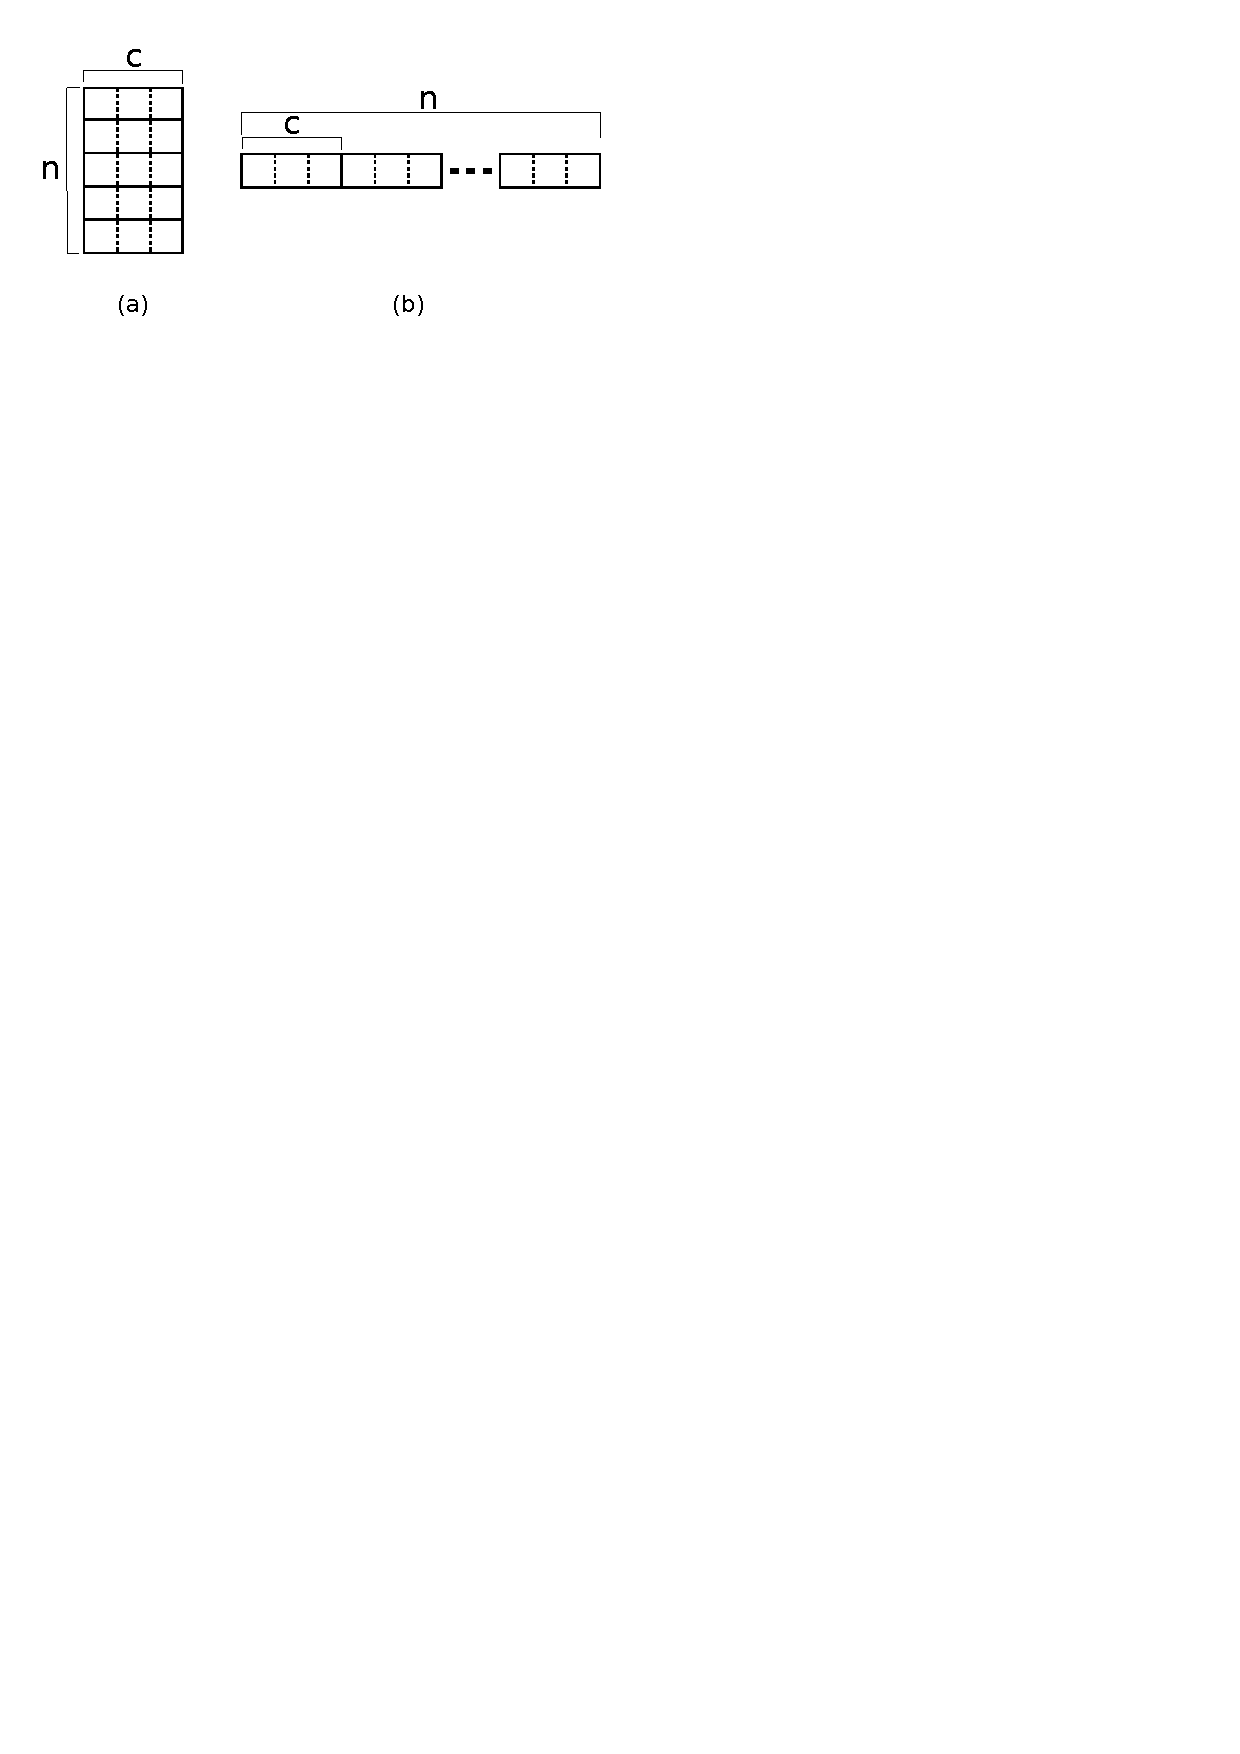
\includegraphics{figures/vectors}
%   \caption{View of  a Vector of size  n and c compenents,  (a) representation of
%     the vector, (b) representation of the storage of the same Vector.}
%   \label{fig:vectors}
% \end{figure}

% All the  data are linerarized  in memory in  an array called values.  This class
% member is public.  So for a Vector  of size $n$ and $c$ component, to access the
% $j^{th}$  component of  th  $i^{th}$ tuple,  you have  to  get $values[i  * c  +
% j]$. You  can also  access to this  value with  accessor \code{at(i, j)}  or the
% constant accessor \code{get(i, j)}.

% If  you want to  store a  matrix on  each tuple  you have  to linearize  it. For
% exemple if you want to store a m * k matrix on each tuple you must specify c = m
% * k.  To access a particular value  in a matrix of  a tuple you will  have to do
% something like $values[ i * m * k + j_i * m + j_j]$.

% \subsubsection{Vector storage convention within FE object\label{sec:FE-convention}}

% The point of  this section is to describe the convention  of storage for vectors
% intented  to be  passed to  {\bf  FE} object  methods.  Indeed  a convention  of
% necessary  since gradient  operators or  integrtaion loops  will use  vectors as
% input and ouput.   Such vectors will be ordered with  a specific convention that
% we intend to describe now.

% For  vector objects,  the  size of  the vector  is  always the  number of  nodes
% associated.  The number  of components  is related  to the  order of  the tensor
% considered. For a scalar  field it is 1, for a vectorial  field, the size of the
% vector is the number of components. For a $m\times n$ matrix field the number of
% components is $m\times n$.

% One common operation  is the manipulation of continuum  fields at the quadrature
% point  positions.   Here  the  size   of  the  vector  is   $mn\_element  \times
% nb\_quad\_points$  and  the  number  of  components is  related  to  the  stored
% object.  For instance the  method \verb$interpolateOnQuadraturePoints()$  take a
% nodal field  stored in a  vector($n\_nodes$,$dim$) and return  a vector($n\_elem
% \times n\_quads$,$dim$).

% Basic gradient operations, like method \verb$gradientOnQuadraturePoints()$, will
% take  as input a  vector($n\_nodes$,$dim$) and  return a  vector($n\_elem \times
% n\_quads$,$dim \times spatial\_dimension$) where spatial dimension is the number
% of dimension in which the domain is embedded.

% In  the  same  way   the  integration  routines  expect  vector($n\_elem  \times
% n\_quads$,$dim$)  and  will  return vector($n\_elem$,$dim$).   For  non-Gaussian
% integrations, the input  by be direction a nodal field.   (At present time, only
% gaussian integrators are implemented within akantu).

% Last but  not the least  is the vectorial  assembly process for which  accept as
% input vector($n\_elem \times n\_quads \times n\_nodes\_per\_element$,$dim$)
% and will return a vector($n\_nodes$,$dim$) nodal object.\\

% {\bf The general convention is that  the number of component shall always be the
%   size of  the object manipulated  at the lowest  level.  The object could  be a
%   per-element, of  per quadrature point  or even per  node basis this  will also
%   apply    as   shown    below.   The    figures    \ref{fig:vector-chain}   and
%   \ref{fig:interpolate-storage} shows the  pattern of the vectors is  the case a
%   interpolation on quadrature points.}

% \begin{figure}
%   \begin{equation}
%     \left(
%       \begin{array}{c}
%         N_1 \\
%         \vdots \\
%         N_I
%         \left\{
%           \begin{array}{c}
%             a_1 \\
%             \vdots \\
%             a_{dim} \\
%           \end{array}
%         \right. \\
%         \vdots \\
%         N_{nb\_nodes}
%       \end{array}
%     \right)
%     \begin{array}{c}
%       \Longrightarrow \\
%       interpolate\\
%       On\\
%       Quadrature\\
%       Points\\
%     \end{array}
%     \left(
%       \begin{array}{c}
%         E_1 \\
%         \vdots \\
%         E_e
%         \left\{
%           \begin{array}{c}
%             q_1 \\
%             \vdots \\
%             \left.
%               \begin{array}{c}
%                 a_1 \\
%                 \vdots \\
%                 a_{dim}
%               \end{array}
%             \right\} q_i \\
%             \vdots \\
%             q_p \\
%           \end{array}
%         \right.  \\
%         \vdots \\
%         E_{nb\_elements}
%       \end{array}
%     \right)
%   \end{equation}
%   \caption{\label{fig:vector-chain}Pattern   of   vectors   manipulated   during
%     interpolation on  quadrature points.  Symbols  N (resp. E, q)  denotes nodes
%     (resp. elements, quadrature points).}
% \end{figure}

% \begin{figure}[!htb]
%   \centering
%   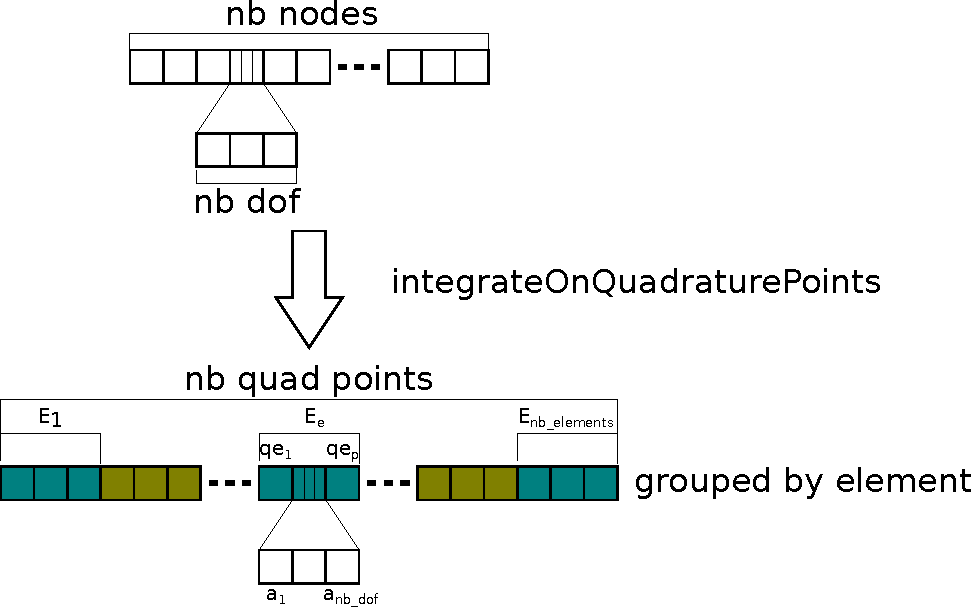
\includegraphics[width=\textwidth]{figures/interpolate}
%   \caption{Input and output  vector of interpolateOnQuadraturePoints. The output
%     Vector has nb\_quadrature\_points tuples,  the quadrature points are grouped
%     by elements (p is the number of quadrature points per element).}
%   \label{fig:interpolate-storage}
% \end{figure}


% The planning to write the documentation
%\chapter{Planning}

\begin{description}
\item[03/12/12] Cyprien: Explicit time integration scheme
\item[03/29/12] Aurelia: Boundary conditions
\item[04/13/12] Leonardo: Existing constitutive laws
\item[04/20/12] Mohadeseh: Adding a constitutive law
\item[04/27/12] Peter: Adding an element
\item[05/04/12] Till: Structural mechanics model
\item[05/11/12] Guillaume: Heat transfer model
\item[05/18/12] Marco: Cohesive elements
\item[05/25/12] Alejandro: Contact detection
\item[06/01/12] David: Contact resolution
\end{description}

\begin{figure}[!htb]
  \centering
  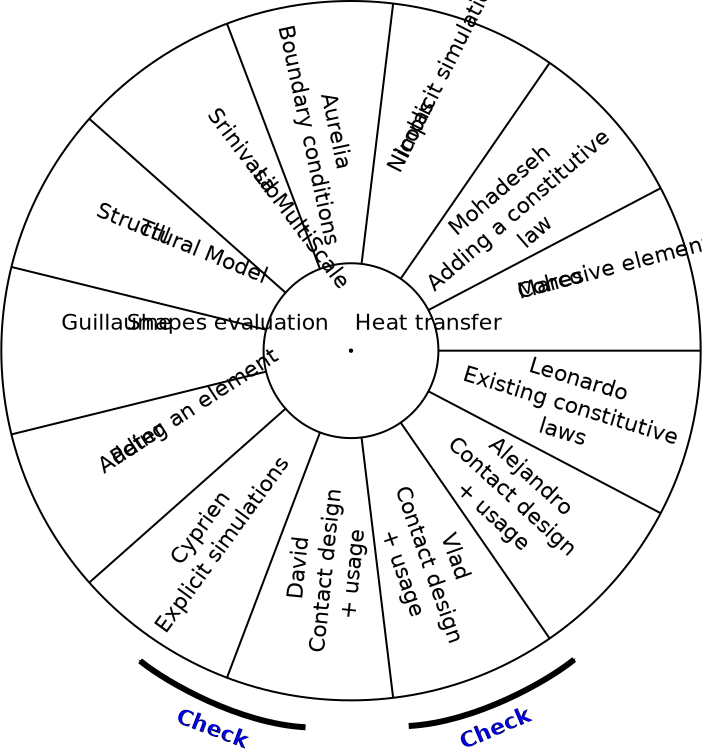
\includegraphics[width=\linewidth]{figures/doc_wheel}
  \caption{Documentation wheel\label{fig:doc_wheel}}
\end{figure}


% The documentation chapter (split in parts)
\chapter{Getting Started}
\section{Downloading the Code}

The \akantu source code can be requested using the form accessible at the URL
\url{http://lsms.epfl.ch/akantu}.  There, you will be asked to accept the LGPL
license terms.

\section{Compiling \akantu}

\akantu is a \code{cmake} project, so to configure it, you can either
follow the usual way:
\begin{command}
  > cd akantu
  > mkdir build
  > cd build
  > ccmake ..
  [ Set the options that you need ]
  > make
  > make install
\end{command}

\noindent Or, use the \code{Makefile} we added for your convenience to
handle the \code{cmake} configuration

\begin{command}
  > cd akantu
  > make config
  > make
  > make install
\end{command}

\noindent All the \akantu options are documented in Appendix
\ref{app:package-dependencies}.


\section{Writing a \texttt{main} Function\label{sect:common:main}}
\label{sec:writing_main}

First of all, \akantu needs to be initialized.  The memory management
included in the core library handles the correct allocation and
de-allocation of vectors, structures and/or objects. Moreover, in
parallel computations, the initialization procedure performs the
communication setup. This is achieved by a pair of functions
(\code{initialize} and \code{finalize}) that are used as follows:
\begin{cpp}
#include "aka_common.hh"
#include "..."

using namespace akantu;

int main(int argc, char *argv[]) {
  initialize("material.dat", argc, argv);

  // your code
  ...

  finalize();
}
\end{cpp}
The \code{initialize} function takes the material file and the program
parameters which can be interpreted by \akantu in due form. Obviously
it is necessary to include all files needed in main. In this manual
all provided code implies the usage of \code{akantu} as namespace.

\section{Creating and Loading a Mesh\label{sect:common:mesh}}

In its current state, \akantu supports three types of meshes: Gmsh~\cite{gmsh},
Abaqus~\cite{abaqus} and Diana~\cite{diana}. Once a \code{Mesh} object is
created with a given spatial dimension, it can be filled by reading a mesh input file.
The method \code{read} of the class \code{Mesh} infers the mesh type from the file extension. If a non-standard file extension is used, the mesh type has to be specified.

\begin{cpp}
UInt spatial_dimension = 2;
Mesh mesh(spatial_dimension);

// Reading Gmsh files
mesh.read("my_gmsh_mesh.msh");
mesh.read("my_gmsh_mesh", _miot_gmsh);


// Reading Abaqus files
mesh.read("my_abaqus_mesh.inp");
mesh.read("my_abaqus_mesh", _miot_abaqus);

// Reading Diana files
mesh.read("my_diana_mesh.dat");
mesh.read("my_diana_mesh", _miot_diana);
\end{cpp}

The Gmsh reader adds the geometrical and physical tags as mesh data. The physical
values are stored as a \code{UInt} data called \code{tag\_0}, if a string
name is provided it is stored as a \code{std::string} data named
\code{physical\_names}. The geometrical tag is stored as a \code{UInt} data named
\code{tag\_1}.


The Abaqus reader stores the \code{ELSET} in ElementGroups and the \code{NSET}
in NodeGroups. The material assignment can be retrieved from the
\code{std::string} mesh data named \code{abaqus\_material}.

% \akantu supports meshes generated with Gmsh~\cite{gmsh}, a free
% software available at \url{http://geuz.org/gmsh/} where a detailed
% documentation can be found. Consequently, this manual will not provide
% Gmsh usage directions. Gmsh outputs meshes in \code{.msh} format that can be read
% by \akantu. In order to import a mesh, it is necessary to create
% a \code{Mesh} object through the following function calls:
% \begin{cpp}
%   UInt spatial_dimension = 2;
%   Mesh mesh(spatial_dimension);
% \end{cpp}
% The only parameter that has to be specified by the user is the spatial
% dimension of the problem. Now it is possible to read a \code{.msh} file with
% a \code{MeshIOMSH} object that takes care of loading a mesh to memory.
% This step is carried out by:
% \begin{cpp}
%   mesh.read("square.msh");
% \end{cpp}
% where the \code{MeshIOMSH} object is first created before being
% used to read the \code{.msh} file. The mesh file name as well as the \code{Mesh}
% object must be specified by the user.

% The \code{MeshIOMSH} object can also write mesh files. This feature
% is useful to save a mesh that has been modified during a
% simulation. The \code{write} method takes care of it:
% \begin{cpp}
%   mesh_io.write("square_modified.msh", mesh);
% \end{cpp}
% which works exactly like the \code{read} method.

% \akantu supports also meshes generated by
% DIANA (\url{http://tnodiana.com}), but only in reading mode. A similar
% procedure applies where the only
% difference is that the \code{MeshIODiana} object should be used
% instead of the \code{MeshIOMSH} one. Additional mesh readers can be
% introduced into \akantu by coding new \code{MeshIO} classes.

\section{Using \texttt{Arrays}}

Data in \akantu can be stored in data containers implemented by
the \code{Array} class. In its most basic usage, the \code{Array} class
implemented in \akantu is similar to the \code{vector} class of
the Standard Template Library (STL) for C++. A simple \code{Array}
containing a sequence of \code{nb\_element} values (of a given type) can be generated with:
\begin{cpp}
  Array<type> example_array(nb_element);
\end{cpp}
where \code{type} usually is \code{Real}, \code{Int}, \code{UInt} or
\code{bool}. Each value is associated to an index, so that data can be
accessed by typing:

\begin{cpp}
  type & val = example_array(index)
\end{cpp}

\code{Arrays} can also contain tuples of values for each index. In
that case, the number of components per tuple must be specified at the
\code{Array} creation.  For example, if we want to create an
\code{Array} to store the coordinates (sequences of three values) of
ten nodes, the appropriate code is the following:
\begin{cpp}
  UInt nb_nodes = 10;
  UInt spatial_dimension = 3;

  Array<Real> position(nb_nodes, spatial_dimension);
\end{cpp}
In this case the $x$ position of the eighth node number will be given by
\code{position(7, 0)} (in C++, numbering starts at 0 and not
1). If the number of components for the sequences is not specified, the
default value of 1 is used.

It is very common in \akantu to loop over arrays to perform a specific
treatment. This ranges from geometric calculation on nodal quantities
to tensor algebra (in constitutive laws for example).
The \code{Array} object has the possibility to request iterators
in order to make the writing of loops easier and enhance readability.
For instance, a loop over the nodal coordinates can be performed like:
\begin{cpp}
  //accessing the nodal coordinates Array (spatial_dimension components)
  Array<Real> nodes = mesh.getNodes();

  //creating the iterators
  Array<Real>::vector_iterator it  = nodes.begin(spatial_dimension);
  Array<Real>::vector_iterator end = nodes.end(spatial_dimension);

  for (; it != end; ++it){
    Vector<Real> & coords = (*it);

    //do what you need
    ....

  }
\end{cpp}
In that example, each \code{Vector<Real>} is a geometrical array of
size \code{spatial\_dimension} and the iteration is conveniently
performed by the \code{Array} iterator.

The \code{Array} object is intensively used to store second order
tensor values.  In that case, it should be specified that the returned
object type is a matrix when constructing the iterator. This is done
when calling the \code{begin} function. For instance, assuming that we
have a \code{Array} storing stresses, we can loop over the stored
tensors by:

\begin{cpp}
  //creating the iterators
  Array<Real>::matrix_iterator it  = stresses.begin(spatial_dimension,spatial_dimension);
  Array<Real>::matrix_iterator end = stresses.end(spatial_dimension,spatial_dimension);

  for (; it != end; ++it){
    Matrix<Real> & stress = (*it);

    //do what you need
    ....

  }
\end{cpp}
In that last example, the \code{Matrix} objects are
\code{spatial\_dimension} $\times$ \code{spatial\_dimension} matrices.
The light objects \code{Matrix} and \code{Vector} can be used and
combined to do most common linear algebra. If the number of component
is 1, it is possible to use a scalar\_iterator rather than the
vector/matrix one.


In general, a mesh consists of several kinds of elements.
Consequently, the amount of data to be stored can differ for each
element type.  The straightforward example is the connectivity array,
namely the sequences of nodes belonging to each element (linear
triangular elements have fewer nodes than, say, rectangular quadratic
elements etc.).  A particular data structure called
\code{ElementTypeMapArray} is provided to easily manage this kind of
data.  It consists of a group of \code{Arrays}, each associated to an
element type.  The following code can retrieve the
\code{ElementTypeMapArray} which stores the connectivity arrays for a
mesh:
\begin{cpp}
  ElementTypeMapArray<UInt> & connectivities = mesh.getConnectivities();
\end{cpp}
Then, the specific array associated to a given element type can be obtained by
\begin{cpp}
  Array<UInt> & connectivity_triangle = connectivities(_triangle_3);
\end{cpp}
where the first order 3-node triangular element was used in the presented piece
of code.

\subsection{Vector \& Matrix}

The \code{Array} iterators as presented in the previous section can be shaped as
\code{Vector} or \code{Matrix}. This objects represent $1^{st}$ and $2^{nd}$
order tensors. As such they come with some functionalities that we will present
a bit more into detail in this here.

\subsubsection{\texttt{Vector<T>}}

\begin{enumerate}
\item Accessors:
  \begin{itemize}
  \item \code{v(i)} gives the $i^{th}$ component of the vector \code{v}
  \item \code{v[i]} gives the $i^{th}$ component of the vector \code{v}
  \item \code{v.size()} gives the number of component
  \end{itemize}
\item Level 1: (results are scalars)
  \begin{itemize}
  \item \code{v.norm()} returns the geometrical norm ($L_2$)
  \item \code{v.norm<N>()} returns the $L_N$ norm defined as $\left(\sum_i
    |\code{v(i)}|^N\right)^{1/N}$. N can take any positive
    integer value. There are also some particular values for the most commonly
    used norms, \code{L\_1} for the Manhattan norm, \code{L\_2} for the
    geometrical norm and \code{L\_inf} for the norm infinity.
  \item \code{v.dot(x)} return the dot product of \code{v} and \code{x}
  \item \code{v.distance(x)} return the geometrical norm of $\code{v} -
    \code{x}$
  \end{itemize}
\item Level 2: (results are vectors)
  \begin{itemize}
  \item \code{v += s}, \code{v -= s}, \code{v *= s}, \code{v /= s} those are
    element-wise operators that sum, substract, multiply or divide all the
    component of \code{v} by the scalar \code{s}
  \item \code{v += x}, \code{v -= x} sums or substracts the vector \code{x}
    to/from \code{v}
  \item \code{v.mul(A, x, alpha)} stores the result of $\alpha \mat{A} \vec{x}$ in \code{v},
    $\alpha$ is equal to 1 by default
  \item \code{v.solve(A, b)} stores the result of the resolution of the system $\mat{A} \vec{x} =
    \vec{b}$ in \code{v}
  \item \code{v.crossProduct(v1, v2)} computes the cross product of \code{v1} and \code{v2} and
    stores the result in \code{v}
  \end{itemize}
\end{enumerate}

\subsubsection{\texttt{Matrix<T>}}
\begin{enumerate}
\item Accessors:
  \begin{itemize}
  \item \code{A(i, j)} gives the component $A_{ij}$ of the matrix \code{A}
  \item \code{A(i)} gives the $i^{th}$ column of the matrix as a \code{Vector}
  \item \code{A[k]} gives the $k^{th}$ component of the matrix, matrices are
    stored in a column major way, which means that to access $A_{ij}$, $k = i +
    j M$
  \item \code{A.rows()} gives the number of rows of \code{A} ($M$)
  \item \code{A.cols()} gives the number of columns of \code{A} ($N$)
  \item \code{A.size()} gives the number of component in the matrix ($M \times N$)
  \end{itemize}
\item Level 1: (results are scalars)

  \begin{itemize}
  \item \code{A.norm<N>()} returns the $L_N$ norm defined as $\left(\sum_i
    |\code{A(i)}|^N\right)^{1/N}$. N can take any positive
    integer value.
  \item \code{A.norm()} is equivalent to \code{A.norm<L\_2>()}
  \item \code{A.trace()} return the trace of \code{A}
  \item \code{A.det()} return the determinant of \code{A}
  \item \code{A.doubleDot(B)} return the double dot product of \code{A} and
    \code{B}, $\mat{A}:\mat{B}$
  \end{itemize}
\item Level 3: (results are matrices)
  \begin{itemize}
  \item \code{A.eye(s)}, \code{Matrix<T>::eye(s)} fills/creates a matrix with
    the $s\mat{I}$ with $\mat{I}$ the identity matrix
  \item \code{A.inverse(B)} stores $\mat{B}^{-1}$ in \code{A}
  \item \code{A.transpose()} returns  $\mat{A}^{t}$
  \item \code{A.outerProduct(v1, v2)} stores $\vec{v_1} \vec{v_2}^{t}$ in
    \code{A}
  \item \code{C.mul<t\_A, t\_B>(A, B, alpha)}: stores the result of the product of
    \code{A} and code{B} time the scalar \code{alpha} in \code{C}. \code{t\_A}
    and \code{t\_B} are boolean defining if \code{A} and \code{B} should be
    transposed or not.

    \begin{tabular}{ccl}
      \toprule
      \code{t\_A} & \code{t\_B} & result \\
      \midrule
      false & false & $\mat{C} = \alpha \mat{A} \mat{B}$\\
      false & true  & $\mat{C} = \alpha \mat{A} \mat{B}^t$\\
      true  & false & $\mat{C} = \alpha \mat{A}^t \mat{B}$\\
      true  & true  & $\mat{C} = \alpha \mat{A}^t \mat{B}^t$\\
      \bottomrule
    \end{tabular}
  \item \code{A.eigs(d, V)} this method computes the eigenvalues and
    eigenvectors of \code{A} and store the results in \code{d} and \code{V} such
    that $\code{d(i)} = \lambda_i$ and $\code{V(i)} = \vec{v_i}$ with
    $\mat{A}\vec{v_i} = \lambda_i\vec{v_i}$ and $\lambda_1 > ... > \lambda_i >
    ... > \lambda_N$
  \end{itemize}
\end{enumerate}


\section{Manipulating group of nodes and/or elements}
\akantu provides the possibility to manipulate
subgroups of elements and nodes.
Any \code{ElementGroup} and/or \code{NodeGroup} must be managed
by a \code{GroupManager}. Such a manager has the role to
associate group objects to names. This is a useful feature,
in particular for the application of the boundary conditions,
as will be demonstrated in section \ref{sect:smm:boundary}.
To most general group manager is the \code{Mesh} class
which inheritates from the \code{GroupManager} class.

For instance, the following code shows how to request
an element group to a mesh:

\begin{cpp}
  // request creation of a group of nodes
  NodeGroup & my_node_group = mesh.createNodeGroup("my_node_group");
  // request creation of a group of elements
  ElementGroup & my_element_group = mesh.createElementGroup("my_element_group");

  /* fill and use the groups */
\end{cpp}


\subsection{The \texttt{NodeGroup} object}
A group of nodes is stored in \code{NodeGroup} objects.
They are quite simple objects which store the indexes
of the selected nodes in a \code{Array<UInt>}.
Nodes are selected by adding them when calling
\code{NodeGroup::add}. For instance you can select nodes
having a positive $X$ coordinate with the following code:
\begin{cpp}
  Array<Real> & nodes = mesh.getNodes();
  NodeGroup & group = mesh.createNodeGroup("XpositiveNode");

  Array<Real>::const_vector_iterator it  = nodes.begin(spatial_dimension);
  Array<Real>::const_vector_iterator end = nodes.end(spatial_dimension);

  UInt index = 0;

  for (; it != end ; ++it , ++index){
    const Vector<Real> & position = *it;
    if (position(0) > 0) group.add(index);
  }
\end{cpp}

\subsection{The \texttt{ElementGroup} object}
A group of elements is stored in \code{ElementGroup} objects.
Since a group can contain elements of various types
the \code{ElementGroup} object stores indexes in
a \code{ElementTypeMapArray<UInt>} object.
Then elements can be added to the group by calling \code{addElement}.

For instance, selecting the elements for which the barycenter of the nodes
has a positive $X$ coordinate can be made with:

\begin{cpp}
  ElementGroup & group = mesh.createElementGroup("XpositiveElement");

  Mesh::type_iterator it  = mesh.firstType();
  Mesh::type_iterator end = mesh.lastType();

  Vector<Real> barycenter(spatial_dimension);

  for(; it != end; ++it){
    UInt nb_element  = mesh.getNbElement(*it);
    for(UInt e = 0; e < nb_element; ++e) {
      ElementType type = *it;
      mesh.getBarycenter(e, type, barycenter.storage());
      if (barycenter(0) > 0) group.add(type,e);
    }
  }
\end{cpp}



%%% Local Variables:
%%% mode: latex
%%% TeX-master: "manual"
%%% End:

\chapter{Elements\index{Elements}}

The base for every Finite Elements computation is its mesh and the elements that are used within that mesh. The element types that can be used depend on the mesh, but also on the dimensionality of the problem (1D, 2D or 3D). In \akantu several isoparametric Langrangian element types are supported (and one serendipity element). Each of these types is discussed in some detail below, starting with the 1D-elements all the way to the 3D-elements. More detailed information (shape function, location of Gaussian quadrature points, and so on) can be found in Appendix~\ref{app:elements}.

%%%%%%%%%% 1D %%%%%%%%%
\section{Isoparametric Elements\index{Elements!Isoparametric}}

\subsection*{1D\index{Elements!1D}}

In \akantu there are two types of isoparametric elements defined in 1D. These element types are called \code{\_segment\_2} and \code{\_segment\_3} and are depicted schematically in Figure~\ref{fig:elements:1D}. Some of the basic properties of these elements are listed in Table~\ref{tab:elements:1D}.

\begin{figure}[!htb]
\begin{center}
\begin{tabular}{m{0.3\textwidth}m{0.1\textwidth}m{0.3\textwidth}}
\subfloat[\code{\_segment\_2}]{
  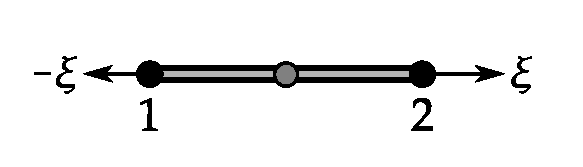
\includegraphics[width=0.3\textwidth]{figures/elements/segment_2}
  \label{fig:elements:segment2}
} & &
\subfloat[\code{\_segment\_3}]{
  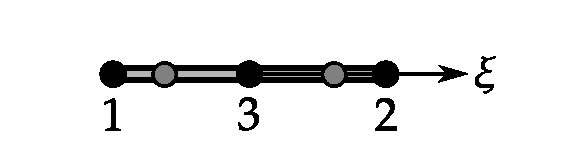
\includegraphics[width=0.3\textwidth]{figures/elements/segment_3}
  \label{fig:elements:segment3}
}
\end{tabular}
\end{center}
\caption{Schematic overview of the two 1D element types in \akantu. In each element the node numbering as used in \akantu is indicated and also the quadrature points are highlighted (gray circles).}
\label{fig:elements:1D}
\end{figure}

\begin{table}[!htb]
\begin{center}
\begin{tabular}{l|ccc}
\toprule
Element type & Order & \# nodes & \# quad. points \\
\midrule
\texttt{\_segment\_2} & linear & 2 & 1 \\
\texttt{\_segment\_3} & quadratic & 3 & 2 \\
\bottomrule
\end{tabular}
\end{center}
\caption{Some basic properties of the two 1D isoparametric elements in \akantu.}
\label{tab:elements:1D}
\end{table}

%%%%%%%%%% 2D %%%%%%%%%
\subsection*{2D\index{Elements!2D}}

In \akantu there are four types of isoparametric elements defined in 2D. These element types are called \code{\_triangle\_3}, \code{\_triangle\_6}, \code{\_quadrangle\_4} and \code{\_quadrangle\_8} and all of them are depicted in Figure~\ref{fig:elements:2D}. As with the 1D elements, some of the most basic properties of these elements are listed in Table~\ref{tab:elements:2D}. It is important to note that the first element is linear, the next two quadratic and the last one cubic. Furthermore, the last element type (\code{\_quadrangle\_8}) is not a Langrangian but a serendipity element.

\begin{figure}[!htb]
\begin{center}
\begin{tabular}{m{0.3\textwidth}m{0.1\textwidth}m{0.3\textwidth}}
\subfloat[\code{\_triangle\_3}]{
  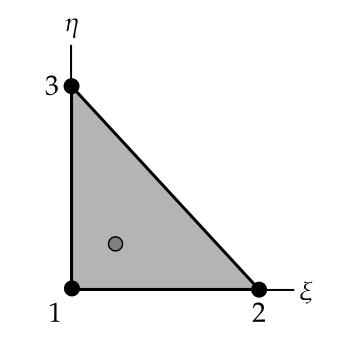
\includegraphics[width=0.3\textwidth]{figures/elements/triangle_3}
  \label{fig:elements:triangle3}
} & &
\subfloat[\code{\_triangle\_6}]{
  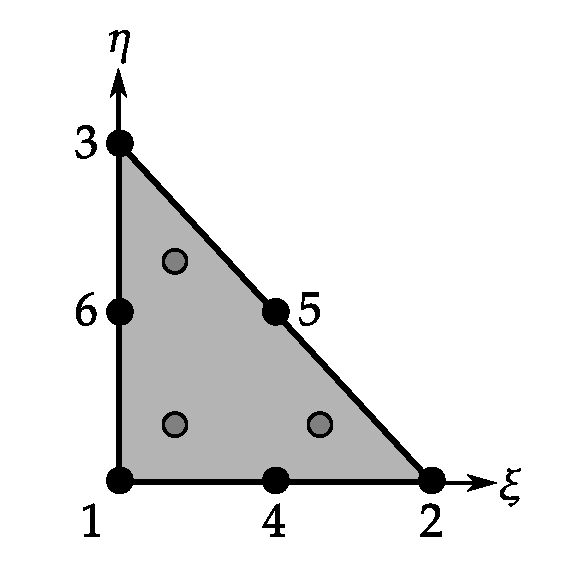
\includegraphics[width=0.3\textwidth]{figures/elements/triangle_6}
  \label{fig:elements:triangle6}
} \\
\subfloat[\code{\_quadrangle\_4}]{
  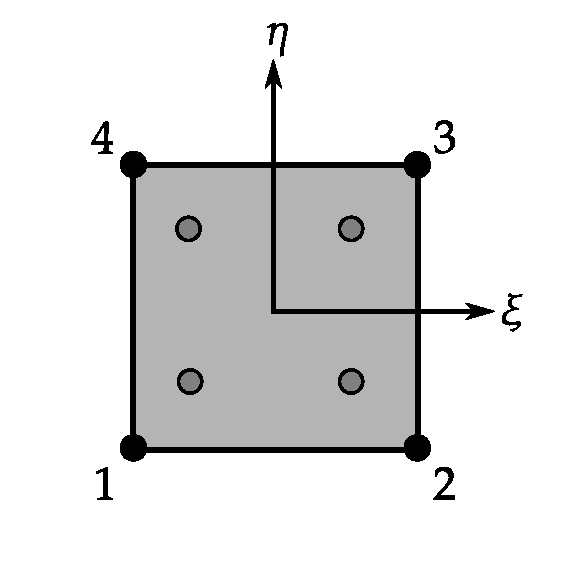
\includegraphics[width=0.3\textwidth]{figures/elements/quadrangle_4}
  \label{fig:elements:quadrangle4}
} & &
\subfloat[\code{\_quadrangle\_8}]{
  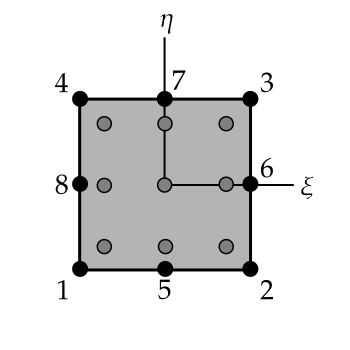
\includegraphics[width=0.3\textwidth]{figures/elements/quadrangle_8}
  \label{fig:elements:quadrangle8}
}
\end{tabular}
\end{center}
\caption{Schematic overview of the four 2D element types in \akantu. In each element the node numbering as used in \akantu is indicated and also the quadrature points are highlighted (gray circles).}
\label{fig:elements:2D}
\end{figure}

\begin{table}[!htb]
\begin{center}
\begin{tabular}{l|ccc}
\toprule
Element type & Order & \# nodes & \# quad. points \\
\midrule
\texttt{\_triangle\_3} & linear & 3 & 1 \\
\texttt{\_triangle\_6} & quadratic & 6 & 3 \\
\hline
\texttt{\_quadrangle\_4} & quadratic & 4 & 4 \\
\texttt{\_quadrangle\_8} & cubic & 8 & 9 \\
\bottomrule
\end{tabular}
\end{center}
\caption{Some basic properties of the four 2D isoparametric elements in \akantu.}
\label{tab:elements:2D}
\end{table}

%%%%%%%%%% 3D %%%%%%%%%
\subsection*{3D\index{Elements!3D}}

In \akantu there are three types of isoparametric elements defined in 3D. These element types are called \code{\_tetrahedron\_4}, \code{\_tetrahedron\_10} and \code{\_hexahedron\_8} and all of them are depicted schematically in Figure~\ref{fig:elements:3D}. As with the 1D and 2D elements some of the most basic properties of these elements are listed in Table~\ref{tab:elements:3D}.

\begin{figure}[!htb]
\begin{center}
\begin{tabular}{m{0.3\textwidth}m{0.3\textwidth}m{0.3\textwidth}}
\subfloat[\code{\_tetrahedron\_4}]{
  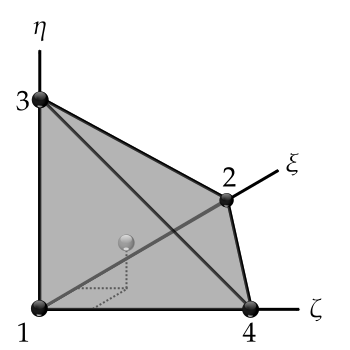
\includegraphics[width=0.3\textwidth]{figures/elements/tetrahedron_4}
  \label{fig:elements:tetrahedron4}
} &
\subfloat[\code{\_tetrahedron\_10}]{
  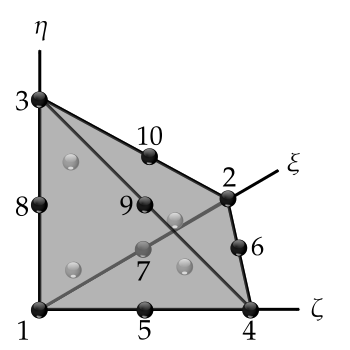
\includegraphics[width=0.3\textwidth]{figures/elements/tetrahedron_10}
  \label{fig:elements:tetrahedron10}
} &
\subfloat[\code{\_hexahedron\_8}]{
  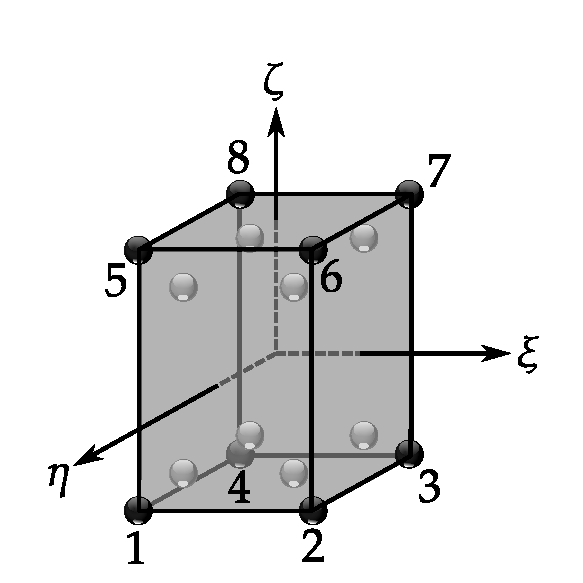
\includegraphics[width=0.3\textwidth]{figures/elements/hexahedron_8}
  \label{fig:elements:hexahedron8}
}
\end{tabular}
\caption{Schematic overview of the three 3D element types in \akantu. In each element the node numbering as used in \akantu is indicated and also the quadrature points are highlighted (gray spheres).}
\label{fig:elements:3D}
\end{center}
\end{figure}

\begin{table}[!htb]
\begin{center}
\begin{tabular}{l|ccc}
\toprule
Element type & Order & \# nodes & \# quad. points  \\
\midrule
\texttt{\_tetrahedron\_4} & linear & 4 & 1  \\
\texttt{\_tetrahedron\_10} & quadratic & 10 & 4  \\
\hline
\texttt{\_hexahedron\_8} & cubic & 8 & 8  \\
\bottomrule
\end{tabular}
\end{center}
\caption{Some basic properties of the three 3D isoparametric elements in \akantu.}
\label{tab:elements:3D}
\end{table}


%%%%%%%%%% COHESIVE ELEMENTS %%%%%%%%%
\IfFileExists{manual-cohesive_elements.tex}{
\section{Cohesive elements}

Cohesive elements are a numerical tool that lets a crack propagate
along the edges of standard elements. The cohesive elements that have
been implemented in Akantu are based on the work of Ortiz and
Pandolfi~\cite{ortiz1999}.

\begin{figure}
  \centering
  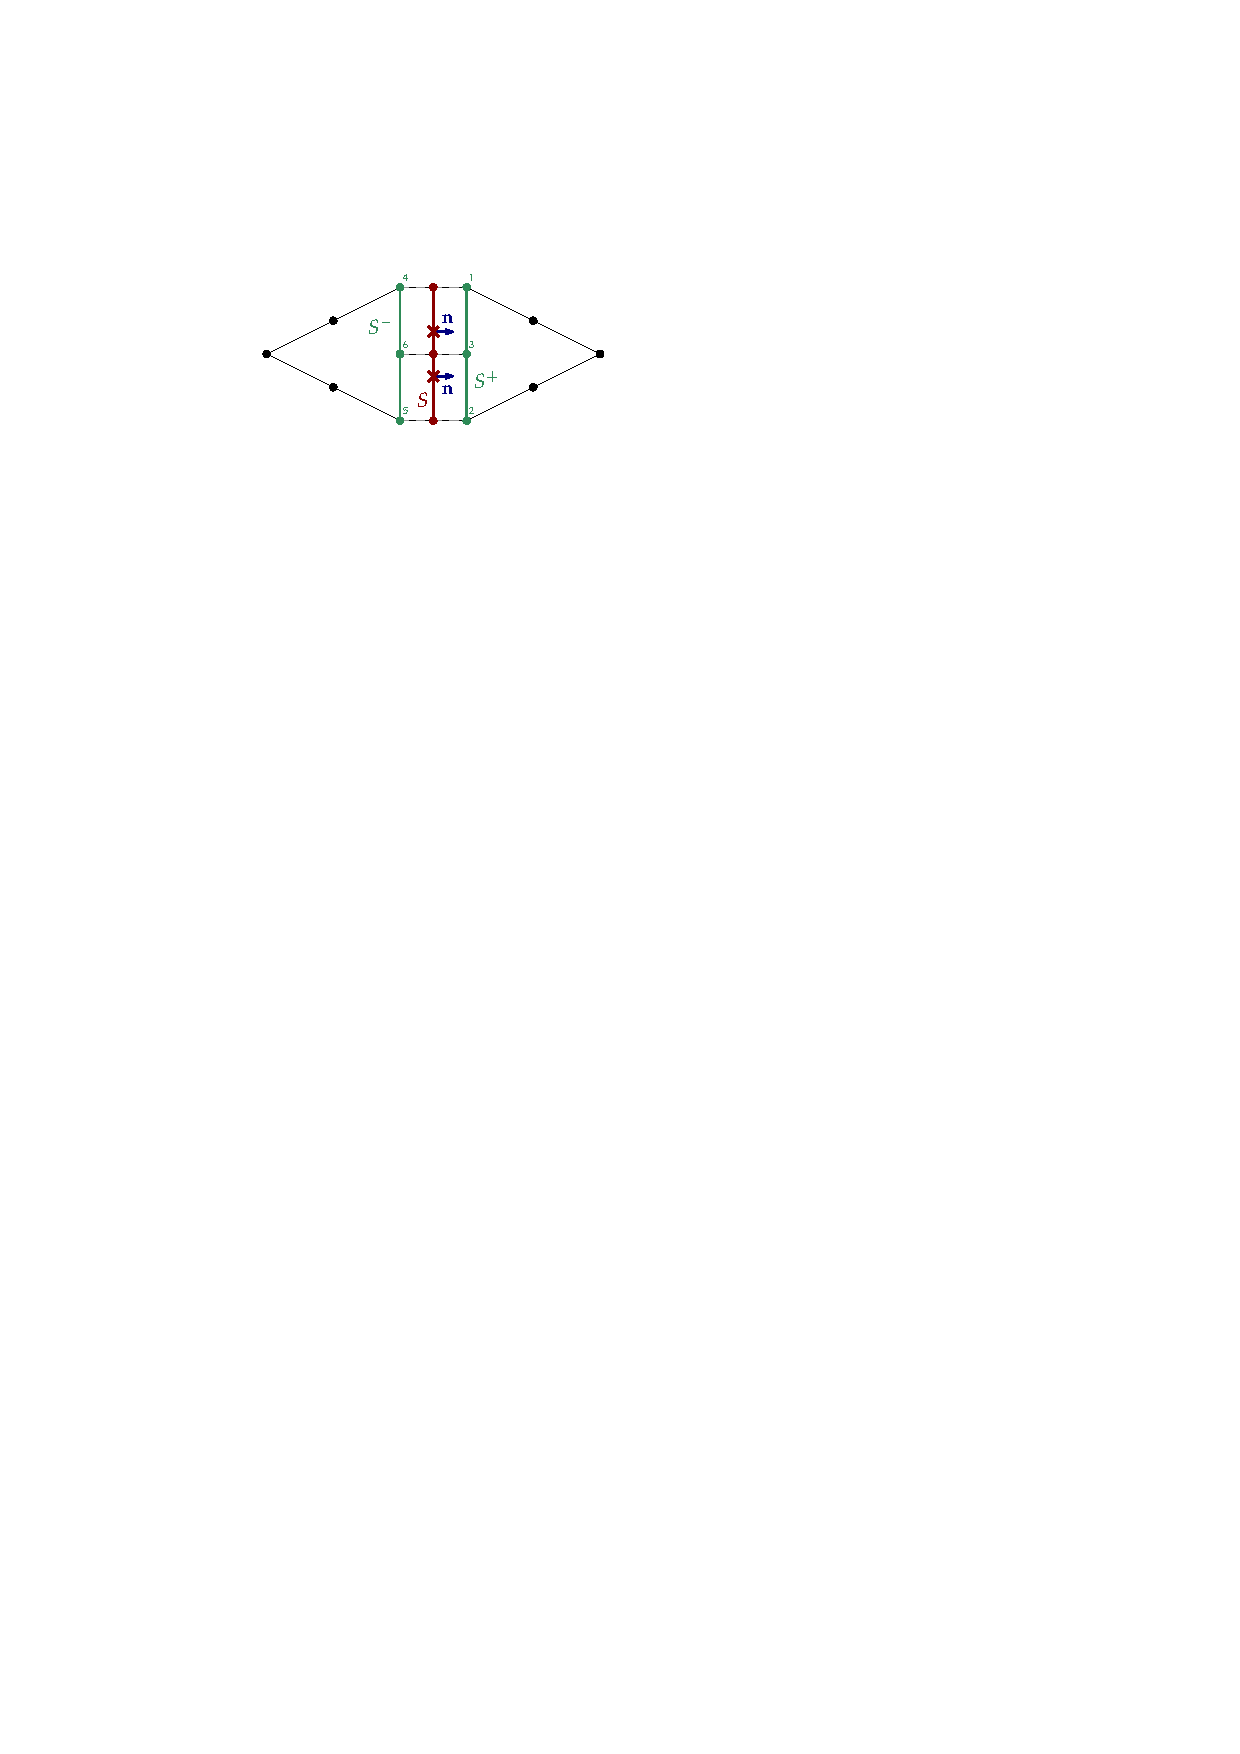
\includegraphics[width=.6\textwidth]{figures/cohesive2d}
  \caption{Cohesive element in 2D for quadratic triangular elements
    T6.}
  \label{fig:smm:coh:cohesive2d}
\end{figure}

\begin{figure}
  \centering
  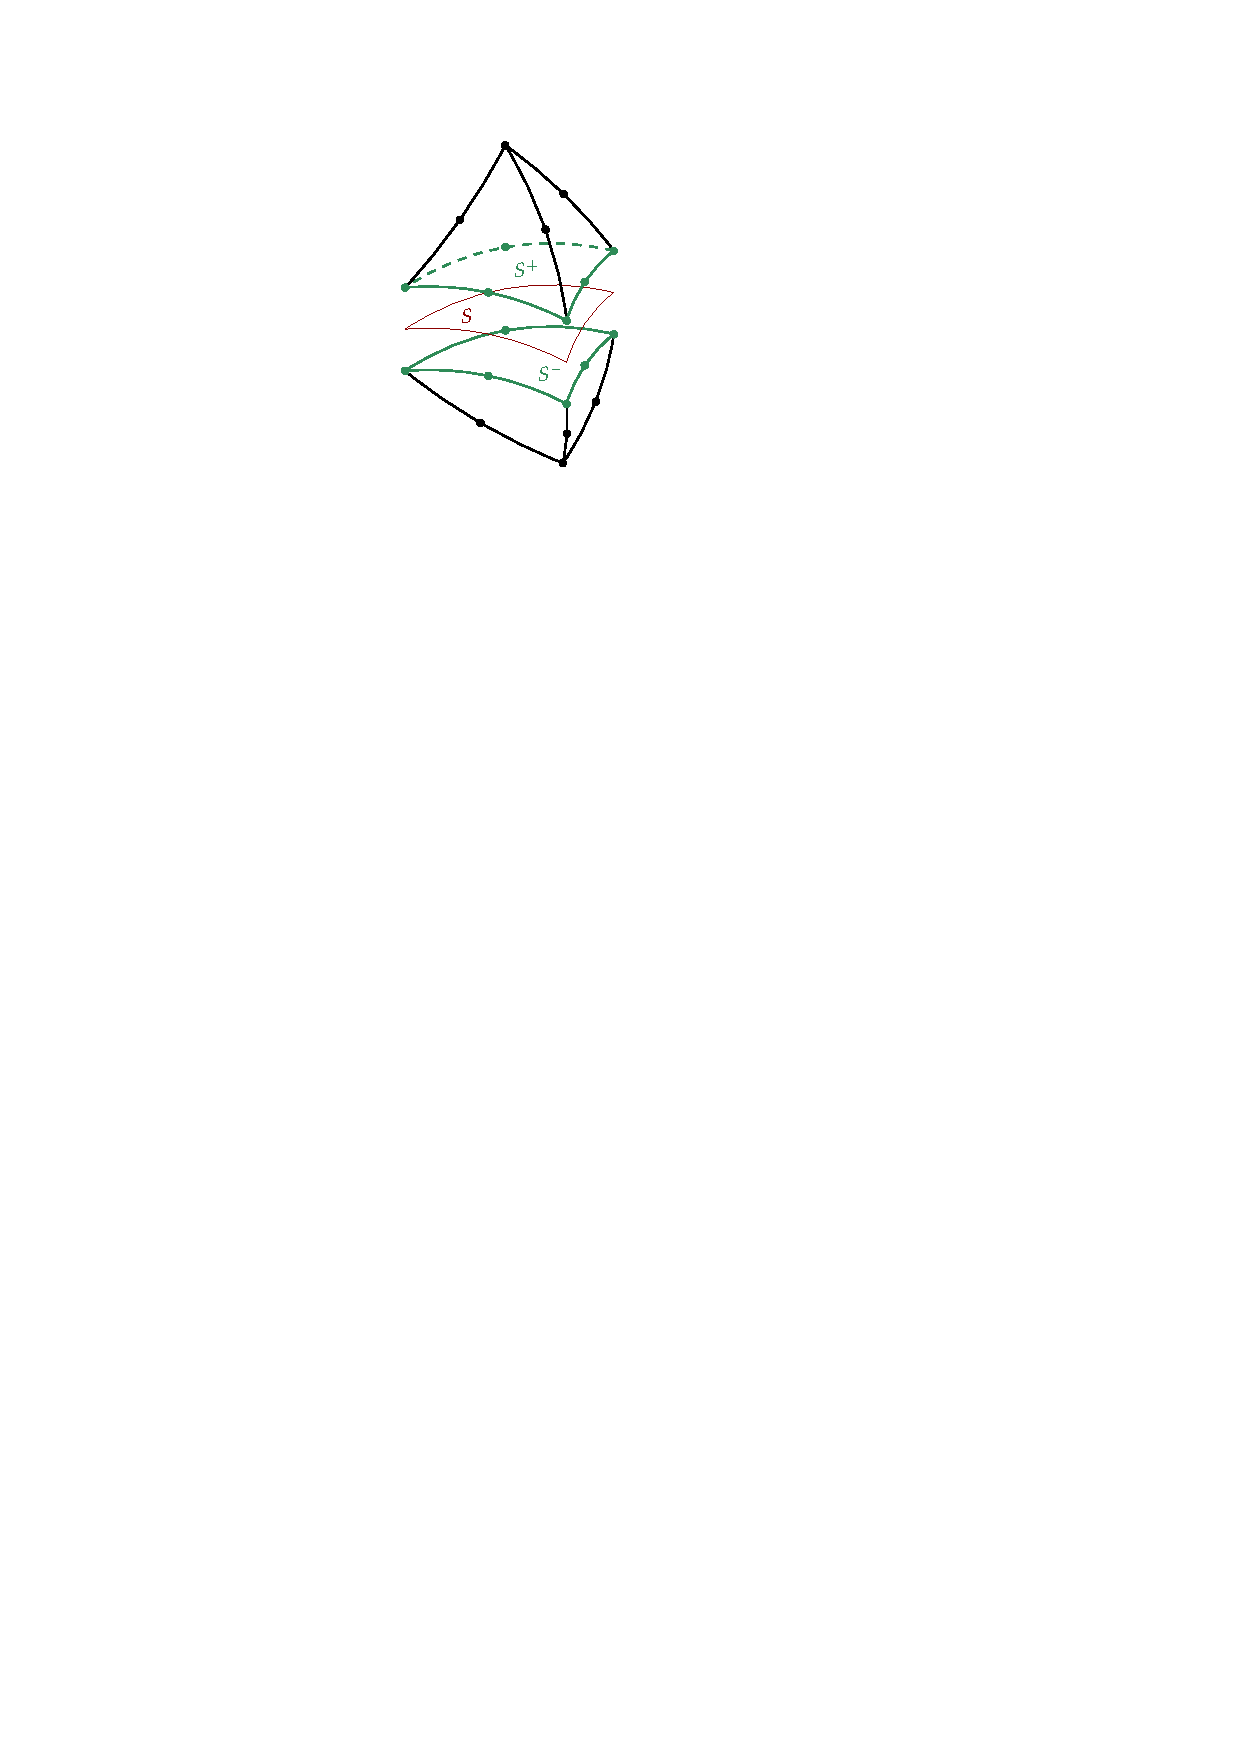
\includegraphics[width=.25\textwidth]{figures/cohesive3d}
  \caption{Cohesive element in 3D for quadratic tetrahedrons T10.}
  \label{fig:smm:coh:cohesive3d}
\end{figure}

Cohesive elements consist of a couple of surface elements which are
coincident in space when the opening displacement is zero. Two
schematics of cohesive elements in 2D and 3D can be seen in
figures~\ref{fig:smm:coh:cohesive2d}
and~\ref{fig:smm:coh:cohesive3d}. The two surface elements, denoted by
$S^-$ and $S^+$, must be of the same type and they correspond to the
facet element of the standard elements. All the computations are done
on the middle surface $S$, whose nodal coordinates are just the
average between those of $S^+$ and $S^-$.

In order to track normal and tangential openings, it is convenient to
define a unique normal direction $\vec{n}$ for each quadrature point
of the cohesive element. By convention the normal points from $S^-$ to
$S^+$. The opening displacement vector is:
\begin{equation}
  \label{eq:opening_displacement}
  \vec{\Delta} (\vec{s}) = \sum_{n=1}^N \llbracket \vec{x}_n \rrbracket N_n (\vec s)
\end{equation}
where $N_n$ are the shape functions of the cohesive element (they are
exactly the same of those of a single surface element) and
\begin{equation}
  \label{eq:disp_difference}
  \llbracket \vec{x}_n \rrbracket = \vec{x}_n^+ - \vec{x}_n^-
\end{equation}
in which $\vec{x}_n^\pm$ for $n=1,\dots,N$ are the current coordinates
of the nodes.

The quantities that have been defined so far are sufficient to
completely define the cohesive tractions per unit deformed
area. As the tangential direction $\vec{t}$ depends on the normal one
$\vec{n}$, equation~\eqref{eq:smm:coh:tractions} can be rewritten as:
\begin{equation}
  \vec{T} = \left[ \frac{\beta^2}{\kappa} \vec{\Delta} +
    \left( 1- \frac{\beta^2}{\kappa}\right)
    \left( \vec{\Delta} \cdot \vec{n}\right) \vec{n} \right]
  \frac{\sigma_\mathrm{c}}{\delta}
  \left( 1- \frac{\delta}{\delta_\mathrm{c}} \right) =
  \vec{T}(\vec{\Delta}, \vec{n})
\end{equation}
 By interpolation it is now possible to derive the nodal
forces as:
\begin{equation}
  f_{in}^\pm = \mp \int_{S_0} T_i N_n\, \mathrm{d}S_0
\end{equation}
in which the integral extends over the undeformed middle surface $S_0$
of the cohesive element.

\begin{figure}
  \centering
  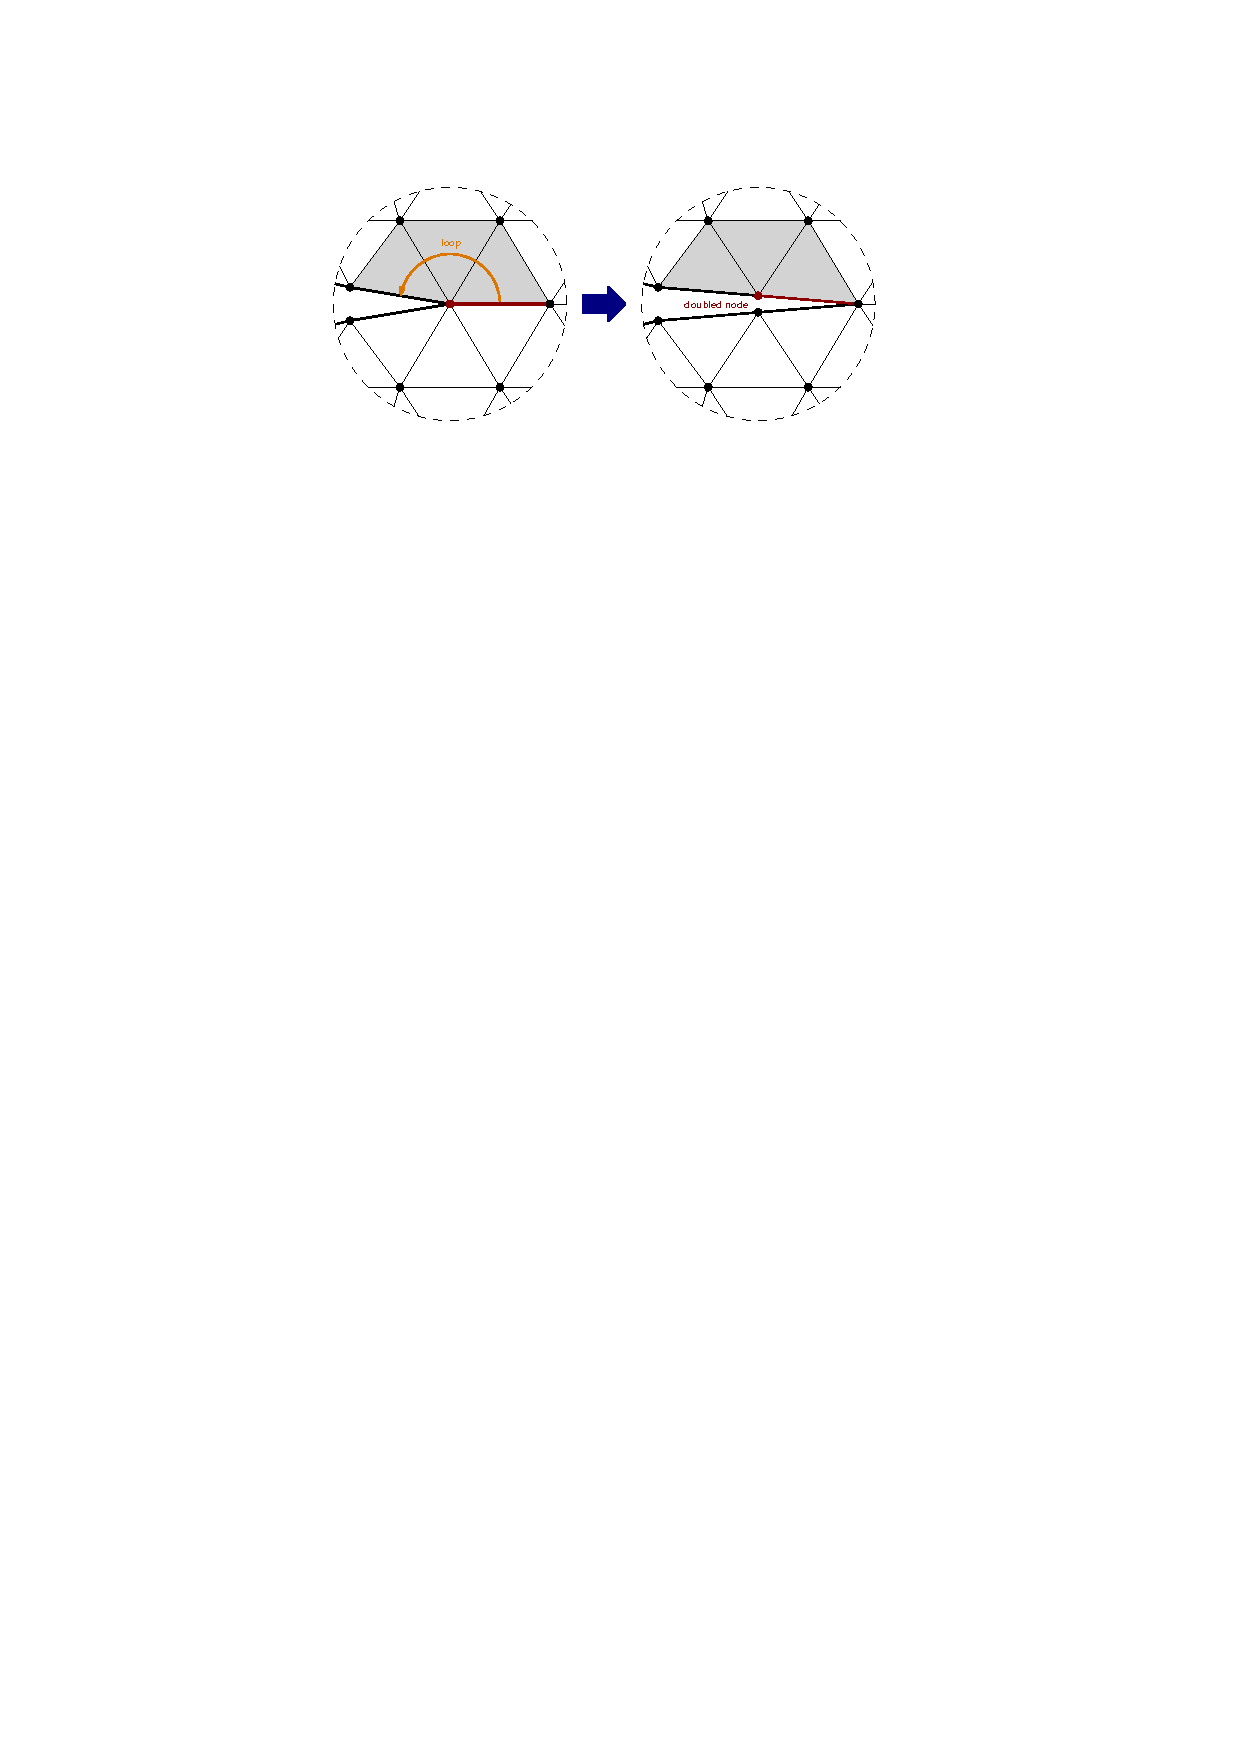
\includegraphics[width=.9\textwidth]{figures/insertion}
  \caption{Insertion of a cohesive element.}
  \label{fig:smm:coh:insertion}
\end{figure}

Cohesive element insertion can be either realized at the beginning of
the simulation or it can be carried out dynamically during the
simulation. The first approach is called \emph{intrinsic} while the
second one \emph{extrinsic}. When an element is present from the
beginning, a bilinear or exponential cohesive law should be used
instead of a linear one. A bilinear law works exactly like a linear
one except for an additional parameter $\delta_0$ separating an
initial linear elastic part from the linear irreversible one. The
exponential law will be described later in the manual.

In dynamic cohesive element insertion, normal and tangential stresses
along the edges of standard elements are used to compute the effective
stress
\begin{equation}
  \sigma_\mathrm{eff} = \sqrt{\sigma_\mathrm{n}^2 +
    \frac{\tau_\mathrm{nt}^2}{\beta^2}}
\end{equation}
where the indexes $n$ and $t$ respectively refer to normal and
tangential directions. Obviously, if $\sigma_\mathrm{n}$ is
compressive, its contribution is not considered. The so computed
effective stress $\sigma_\mathrm{eff}$ is monitored, and when it
overcomes a threshold stress on a certain edge a new cohesive element
is inserted. New nodes are added and the element connectivity is
updated (see figure~\ref{fig:smm:coh:insertion}). This topological
mesh changing technique is very convenient because it allows
simulating crack propagation without remeshing the domain.

\begin{table}[!htb]
\begin{center}
\begin{tabular}{l|llcc}
\toprule
Element type & Facet type & Order & \# nodes & \# quad. points  \\
\midrule
\texttt{\_cohesive\_1d\_2} & \texttt{\_point\_1} & linear & 2 & 1  \\
\hline
\texttt{\_cohesive\_2d\_4} & \texttt{\_segment\_2} & linear & 4 & 1  \\
\texttt{\_cohesive\_2d\_6} & \texttt{\_segment\_3} & quadratic & 6 & 2  \\
\hline
\texttt{\_cohesive\_3d\_6} & \texttt{\_triangle\_3} & linear & 6 & 1  \\
\texttt{\_cohesive\_3d\_12} & \texttt{\_triangle\_6} & quadratic & 12 & 3  \\
\bottomrule
\end{tabular}
\end{center}
\caption{Some basic properties of the cohesive elements in \akantu.}
\label{tab:cohesive_elements}
\end{table}

%%% Local Variables:
%%% mode: latex
%%% TeX-master: "manual"
%%% End:
}{}

%%%%%%%%%% STRUCTURAL ELEMENTS %%%%%%%%%
\IfFileExists{manual-structuralmechanicsmodel-elements.tex}{\subsection{Structural Elements\index{Elements!Structural}}

\subsubsection*{Bernoulli Beam Elements\index{Elements!Bernoulli}}
These elements allow to compute the displacements and rotations of
structures constituted by Bernoulli beams. \akantu defines them for
both 2D and 3D problems respectively in the element types
\code{\_bernoulli\_beam\_2} and \code{\_bernoulli\_beam\_3}. A
schematic depiction of a beam element is shown in
Figure~\ref{fig:elements:bernoulli} and some of its properties are
listed in Table~\ref{tab:elements:bernoulli}.

\note{Beam elements are of mixed order: the axial displacement is
  linearly interpolated while transverse displacements and rotations
  use cubic shape functions.}

\begin{figure}[htb]
  \centering
  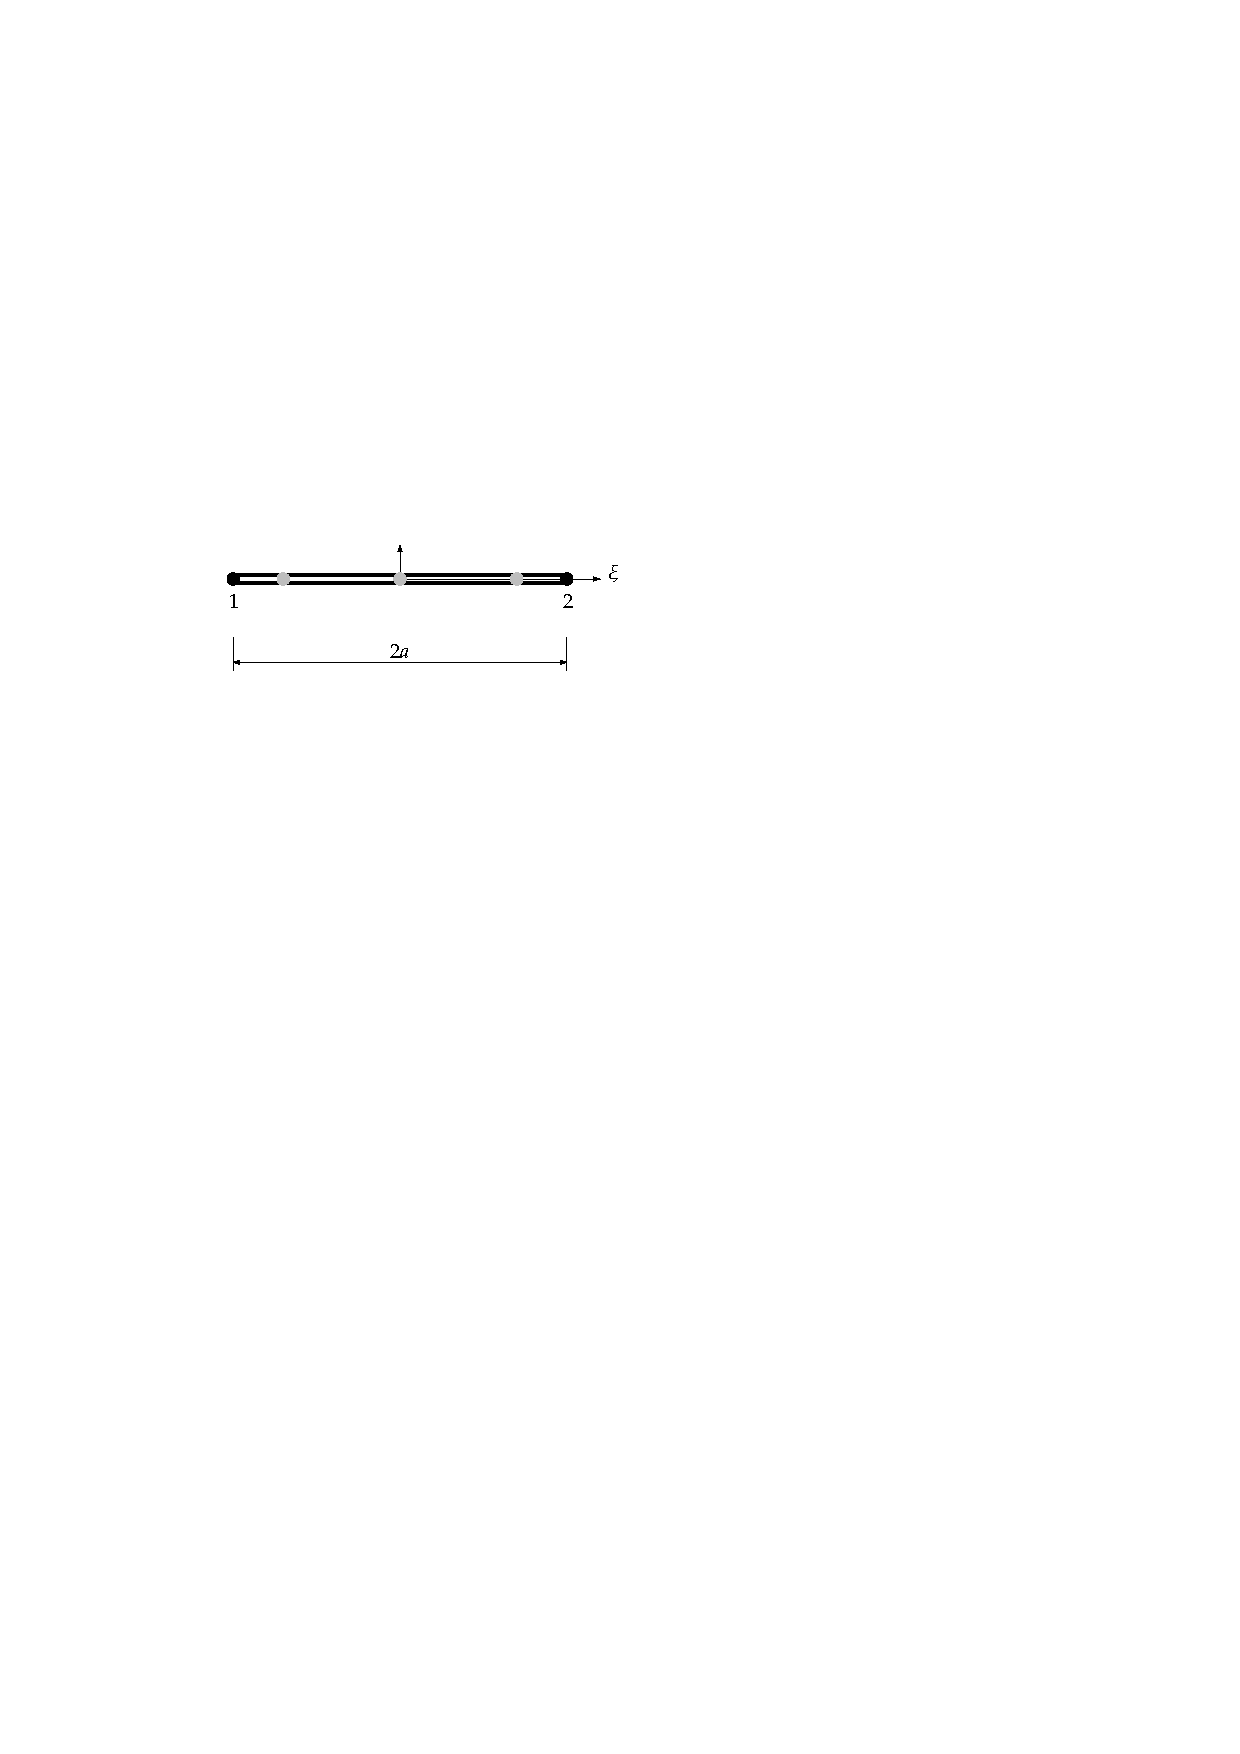
\includegraphics[width=0.3\textwidth]{figures/elements/bernoulli_2}
  \caption{Schematic depiction of a Bernoulli beam element (applied to
    2D and 3D) in \akantu. The node numbering as used in \akantu is
    indicated, and also the quadrature points are highlighted (gray
    circles).}
  \label{fig:elements:bernoulli}
\end{figure}
\begin{table}[htb]
  \centering
  \begin{tabular}{c|cccc}
    \toprule
    Element type                  & Dimension & \# nodes &\# quad. points & \# d.o.f.\\
    \midrule
    \texttt{\_bernoulli\_beam\_2} &         2D&         2&              3&  6\\
    \texttt{\_bernoulli\_beam\_3} &         3D&         2&              3&  12\\
    \bottomrule
  \end{tabular}
  \caption{Some basic properties of the beam elements in \akantu}
  \label{tab:elements:bernoulli}
\end{table}
}{}

%%% Local Variables:
%%% mode: latex
%%% TeX-master: "manual"
%%% End:


%\IfFileExists{manual-lumping.tex}{}{\section{Matrix Lumping Strategies\index{Matrix Lumping Strategies}\label{section:mls} \todo{give lumping strategies description}}
}

\chapter{Solid Mechanics Model\index{SolidMechanicsModel}\label{sect:smm}}

The solid mechanics model is a specific implementation of the
\code{Model} interface dedicated to handle the equations of motion or
equations of equilibrium. The model is created for a given mesh.  It
will create its own \code{FEEngine} object to compute the interpolation,
gradient, integration and assembly operations.  A
\code{SolidMechanicsModel} object can simply be created like this:
\begin{cpp}
  SolidMechanicsModel model(mesh);
\end{cpp}
where \code{mesh} is the mesh for which the equations are to be
solved. A second parameter called \code{spatial\_dimension} can be
added after \code{mesh} if the spatial dimension of the problem is
different than that of the mesh.

This model contains at least the following six \code{Arrays}:
\begin{description}
\item[blocked\_dofs] contains a Boolean value for each degree of
  freedom specifying whether that degree is blocked or not. A
  Dirichlet boundary condition can be prescribed by setting the
  \textbf{blocked\_dofs} value of a degree of freedom to \code{true}.
  A Neumann boundary condition can be applied by setting the
  \textbf{blocked\_dofs} value of a degree of freedom to \code{false}.
  The \textbf{displacement}, \textbf{velocity} and
  \textbf{acceleration} are computed for all degrees of freedom for
  which the \textbf{blocked\_dofs} value is set to \code{false}. For
  the remaining degrees of freedom, the imposed values (zero by
  default after initialization) are kept.
\item[displacement] contains the displacements of all degrees of
  freedom. It can be either a computed displacement for free degrees
  of freedom or an imposed displacement in case of blocked ones
  ($\vec{u}$ in the following).
\item[velocity] contains the velocities of all degrees of freedom.  As
  \textbf{displacement}, it contains computed or imposed velocities
  depending on the nature of the degrees of freedom ($\dot{\vec{u}}$
  in the following).
\item[acceleration] contains the accelerations of all degrees of
  freedom. As \textbf{displacement}, it contains computed or imposed
  accelerations depending on the nature of the degrees of freedom
  ($\ddot{\vec{u}}$ in the following).
\item[force] contains the external forces applied on the nodes
  ($\vec{f}_{\st{ext}}$ in the following).
\item[residual] contains the difference between external and internal
  forces. On blocked degrees of freedom, \textbf{residual} contains
  the support reactions.  ($\vec{r}$ in the following).  It should be
  mentioned that at equilibrium \textbf{residual} should be zero on
  free degrees of freedom.
\end{description}

Some examples to help to understand how to use this model will be
presented in the next sections.

\section{Model Setup}


\subsection{Setting Initial Conditions \label{sect:smm:initial_condition}}

For a unique solution of the equations of motion, initial
displacements and velocities for all degrees of freedom must be
specified:
\begin{eqnarray}
  \vec{u}(t=0) = \vec{u}_0\\
  \dot{\vec u}(t=0) =\vec{v}_0
\end{eqnarray} The solid mechanics model can be initialized as
follows:
\begin{cpp}
  model.initFull()
\end{cpp}
This function initializes the internal arrays and sets them to
zero. Initial displacements and velocities that are not equal to zero
can be prescribed by running a loop over the total number of
nodes. Here, the initial displacement in $x$-direction and the
initial velocity in $y$-direction for all nodes is set to $0.1$ and $1$,
respectively.
\begin{cpp}
Array<Real> & disp = model.getDisplacement();
Array<Real> & velo = model.getVelocity();
for (UInt i = 0; i < mesh.getNbNodes(); ++i) {
  disp(i, 0) = 0.1;
  velo(i, 1) = 1.;
}
\end{cpp}

\subsection{Setting Boundary Conditions\label{sect:smm:boundary}}
This section explains how to impose Dirichlet or Neumann boundary
conditions. A Dirichlet boundary condition specifies the values that
the displacement needs to take for every point $x$ at the boundary
($\Gamma_u$) of the problem domain (Fig.~\ref{fig:smm:boundaries}):
\begin{equation}
  \vec{u} = \bar{\vec u} \quad \forall \vec{x}\in
  \Gamma_{u}
\end{equation}
A Neumann boundary condition imposes the value of the gradient of the
solution at the boundary $\Gamma_t$ of the problem domain
(Fig.~\ref{fig:smm:boundaries}):
\begin{equation}
  \vec{t} = \mat{\sigma} \vec{n} = \bar{\vec t} \quad
  \forall \vec{x}\in \Gamma_{t}
\end{equation}

\begin{figure} \centering
\def\svgwidth{0.5\columnwidth}
  \input{figures/problemDomain.pdf_tex}
  \caption{Problem domain $\Omega$ with boundary in three
    dimensions. The Dirchelet and the Neumann regions of the boundary
    are denoted with $\Gamma_u$ and $\Gamma_t$,
    respecitvely.\label{fig:smm:boundaries}}
  \label{fig:problemDomain}
\end{figure}

Different ways of imposing these boundary conditions exist. A basic
way is to loop over nodes or elements at the boundary and apply local
values. A more advanced method consists of using the notion of the
boundary of the mesh. In the following both ways are presented.

Starting with the basic approach, as mentioned, the Dirichlet boundary
conditions can be applied by looping over the nodes and assigning the
required values. Figure~\ref{fig:smm:dirichlet_bc} shows a beam with a
fixed support on the left side. On the right end of the beam, a load
is applied. At the fixed support, the displacement has a given
value. For this example, the displacements in both the $x$ and the
$y$-direction are set to zero. Implementing this displacement boundary
condition is similar to the implementation of initial displacement
conditions described above. However, in order to impose a displacement
boundary condition for all time steps, the corresponding nodes need to
be marked as boundary nodes using the function \code{blocked}. While, 
in order to impose a load on the right side, the nodes are not marked.
The detail codes are shown as follows:

\begin{cpp}
Array<bool> & blocked = model.getBlockedDOFs();
const Array<Real> & pos = mesh.getNodes();

UInt nb_nodes = mesh.getNbNodes();

for (UInt i = 0; i < nb_nodes; ++i) {
  if(Math::are_float_equal(pos(i, 0), 0)) {
    blocked(i, 0) = true; //block dof in x-direction
    blocked(i, 1) = true; //block dof in y-direction
    disp(i, 0) = 0.; //fixed displacement in x-direction
    disp(i, 1)= 0.; //fixed displacement in y-direction
  } else if (Math::are_float_equal(pos(i, 10), 0)) {
    blocked(i, 0) = false; //unblock dof in x-direction
    forces(i, 0) = 10.; //force in x-direction
  }
}
\end{cpp}

\begin{figure}[!htb]
  \centering
  \includegraphics[scale=0.4]{figures/dirichlet}
  \caption{Beam with fixed support and load.\label{fig:smm:dirichlet_bc}}
\end{figure}


For the more advanced approach, one needs the notion of a boundary in
the mesh. Therefore, the boundary should be created before boundary
condition functors can be applied. Generally the boundary can be
specified from the mesh file or the geometry.  For the first case, the
function \code{createGroupsFromMeshData} is called.  This function
can read any types of mesh data which are provided in the mesh
file. If the mesh file is created with Gmsh, the function takes one
input strings which is either \code{tag\_0}, \code{tag\_1} or
\code{physical\_names}. The first two tags are assigned by Gmsh to
each element which shows the physical group that they belong to. In
Gmsh, it is also possible to consider strings for different groups of
elements. These elements can be separated by giving a string
\code{physical\_names} to the function
\code{createGroupsFromMeshData}:
\begin{cpp}
mesh.createGroupsFromMeshData<std::string>("physical_names").
\end{cpp}
Boundary conditions support can also be
created from the geometry by calling
\code{createBoundaryGroupFromGeometry}. This function gathers all the
elements on the boundary of the geometry.

To apply the required boundary conditions, the function \code{applyBC}
needs to be called on a \code{SolidMechanicsModel}. This function
gets a Dirichlet or Neumann functor and a string which specifies the
desired boundary on which the boundary conditions is to be
applied. The functors specify the type of conditions to apply. Three
built-in functors for Dirichlet exist: \code{FlagOnly, FixedValue,}
and \code{IncrementValue}. The functor \code{FlagOnly} is used if a
point is fixed in a given direction. Therefore, the input parameter to
this functor is only the fixed direction. The \code{FixedValue}
functor is used when a displacement value is applied in a fixed
direction. The \code{IncrementValue} applies an increment to the
displacement in a given direction. The following code shows the
utilization of three functors for the top, bottom and side surface of
the mesh which were already defined in the Gmsh file:

\begin{cpp}
model.applyBC(BC::Dirichlet::FixedValue(13.0, _y), "Top");

model.applyBC(BC::Dirichlet::FlagOnly(_x), "Bottom");

model.applyBC(BC::Dirichlet::IncrementValue(13.0, _x), "Side");
\end{cpp}

To apply a Neumann boundary condition, the applied traction or stress
should be specified before. In case of specifying the traction on the
surface, the functor \code{FromTraction} of Neumann boundary
conditions is called. Otherwise, the functor \code{FromStress} should
be called which gets the stress tensor as an input parameter.

\begin{cpp}
Array<Real> surface_traction(3);
surface_traction(0)=0.0;
surface_traction(1)=0.0;
surface_traction(2)=-1.0;

Matrix<Real> surface_stress(3, 3, 0.0);
surface_stress(0,0)=0.0;
surface_stress(1,1)=0.0;
surface_stress(2,2)=-1.0;

model.applyBC(BC::Neumann::FromTraction(surface_traction), "Bottom");

model.applyBC(BC::Neumann::FromStress(surface_stress), "Top");
\end{cpp}

If the boundary conditions need to be removed during the simulation, a
functor is called from the Neumann boundary condition to free those
boundary conditions from the desired boundary.

\begin{cpp}
 model.applyBC(BC::Neumann::FreeBoundary(), "Side");
\end{cpp}

User specified functors can also be implemented.  A full example for
setting both initial and boundary conditions can be found in
\shellcode{\examplesdir/boundary\_conditions.cc}.  The problem solved
in this example is shown in Fig.~\ref{fig:smm:bc_and_ic}. It consists
of a plate that is fixed with movable supports on the left and bottom
side. On the right side, a traction, which increases linearly with the
number of time steps, is applied. The initial displacement and
velocity in $x$-direction at all free nodes is zero and two
respectively.
\begin{figure}[!htb]
  \centering
  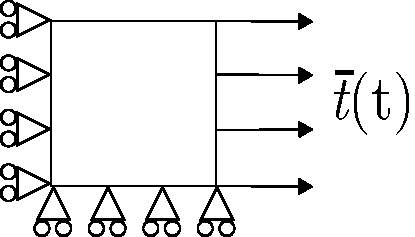
\includegraphics[scale=0.8]{figures/bc_and_ic_example}
  \caption{Plate on movable supports.\label{fig:smm:bc_and_ic}}
\end{figure}

As it is mentioned in Section \ref{sect:common:groups}, node and
element groups can be used to assign the boundary conditions. A
generic example is given below with a Dirichlet boundary condition.

\begin{cpp}
  // create a node group
  NodeGroup & node_group = mesh.createNodeGroup("nodes_fix");

  /* 
  fill the node group with the nodes you want
  */

  // create an element group using the existing node group
  mesh.createElementGroupFromNodeGroup("el_fix", "nodes_fix", spatial_dimension-1);

  // boundary condition can be applied using the element group name
  model.applyBC(BC::Dirichlet::FixedValue(0.0, _x), "el_fix");
\end{cpp}

\subsection{Material Selector\label{sect:smm:materialselector}}

If the user wants to assign different materials to different
finite elements groups in \akantu, a material selector has to be
used. By default, \akantu assigns the first valid material in the
material file to all elements present in the model (regular continuum
materials are assigned to the regular elements and cohesive materials
are assigned to cohesive elements or element facets).

To assign different materials to specific elements, mesh data
information such as tag information or specified physical names can be
used. \code{MeshDataMaterialSelector} class uses this information to
assign different materials. With the proper physical name or tag name
and index, different materials can be assigned as demonstrated in the
examples below.

\begin{cpp}
  MeshDataMaterialSelector<std::string> * mat_selector;
  mat_selector = new MeshDataMaterialSelector<std::string>("physical_names", model);
  model.setMaterialSelector(*mat_selector);
\end{cpp}

In this example the physical names specified in a GMSH geometry file will by
used to match the material names in the input file.

Another example would be to use the first (\code{tag\_0}) or the second
(\code{tag\_1}) tag associated to each elements in the mesh:

\begin{cpp}
  MeshDataMaterialSelector<UInt> * mat_selector;
  mat_selector = new MeshDataMaterialSelector<UInt>("tag_1", model, first_index);
  model.setMaterialSelector(*mat_selector);
\end{cpp}

where \code{first\_index} (default is 1) is the value of \code{tag\_1} that will
be associated to the first material in the material input file. The following
values of the tag will be associated with the following materials.

There are four different material selectors pre-defined in
\akantu. \code{MaterialSelector} and \code{DefaultMaterialSelector} is
used to assign a material to regular elements by default. For the
regular elements, as in the example above,
\code{MeshDataMaterialSelector} can be used to assign different
materials to different elements. 

Apart from the \akantu's default material selectors, users can always
develop their own classes in the main code to tackle various
multi-material assignment situations.

% An application of \code{DefaultMaterialCohesiveSelector} and usage in
% a customly generated material selector class can be seen in
% \shellcode{\examplesdir/cohesive\_element/cohesive\_extrinsic\_IG\_TG/cohesive\_extrinsic\_IG\_TG.cc}.

\IfFileExists{manual-cohesive_elements_insertion.tex}{\subsection{Insertion of Cohesive Elements}
\subsubsection{Dynamics}
As far as dynamic simulations are concerned, cohesive elements are
currently compatible only with the explicit time integration scheme
(see section~\ref{ssect:smm:expl-time-integr}). They do not have to be
inserted when the mesh is generated but during the
simulation. Intrinsic cohesive elements can be introduced at the
beginning of the simulation as follows:
\begin{cpp}
  SolidMechanicsModelCohesive model(mesh);
  model.initFull();
  model.limitInsertion(_x, -1, 1);
  model.insertIntrinsicElements();
\end{cpp}
where the insertion is limited to the facets whose barycenter's $x$
coordinate is in the range $[-1,1]$. Additional restrictions with
respect to $y$ and $z$ directions can be added as well. Similarly the
dynamic insertion of extrinsic cohesive elements can be utilized in
the following way:
\begin{cpp}
  SolidMechanicsModelCohesive model(mesh);
  model.initFull(SolidMechanicsModelCohesiveOptions(_explicit_lumped_mass, true));
  model.limitInsertion(_x, -1, 1);
  model.updateAutomaticInsertion();
\end{cpp}
in which this time the method \code{limitInsertion} prevents the
cohesive elements to be inserted out of the range $[-1,1]$ in the $x$
direction. In order to check stress and automatically insert elements,
it is necessary to call the function \code{checkCohesiveStress} in the
main loop where \code{solveStep} is:
\begin{cpp}
  model.checkCohesiveStress();
  model.solveStep();
\end{cpp}

At any time during the simulation, it is possible to access the
following energies with the relative function:
\begin{cpp}
  Real Ed = model.getEnergy("dissipated");
  Real Er = model.getEnergy("reversible");
  Real Ec = model.getEnergy("contact");
\end{cpp}

\subsubsection{Statics}
The only cohesive law that is applicable in this case is the
exponential one (see
section~\ref{ssect:smm:cl:coh-exponential}). However
unloading-reloading cycles are not supported yet. In this case
cohesive elements have to be inserted before creating the
\code{SolidMechanicsModelCohesive} model:
\begin{cpp}
  Mesh mesh(spatial_dimension);
  mesh.read("implicit_mesh.msh");

  CohesiveElementInserter inserter(mesh);
  inserter.setLimit(_y, 0.9, 1.1);
  inserter.insertIntrinsicElements();

  SolidMechanicsModelCohesive model(mesh);
  model.initFull(SolidMechanicsModelCohesiveOptions(_static));
\end{cpp}
Also in this case the element insertion can be limited to a given
range thanks to the method \code{setLimit}. The first input parameter
of this method indicates the direction while the other two indicate
the extreme values of the range $[0.9, 1.1]$. In order to compute the
energies, the same functions illustrated for dynamics in the last
section can be used.
}{}

\section{Static Analysis\label{sect:smm:static}}

The \code{SolidMechanicsModel} class can handle different analysis
methods, the first one being presented is the static case.  In this
case, the equation to solve is
\begin{equation}
  \label{eqn:smm:static} \mat{K} \vec{u} =
  \vec{f}_{\st{ext}}
\end{equation}
where $\mat{K}$ is the global stiffness matrix, $\vec{u}$ the
displacement vector and $\vec{f}_{\st{ext}}$ the vector of external
forces applied to the system.

To solve such a problem, the static solver of the
\code{SolidMechanicsModel}\index{SolidMechanicsModel} object is used.
First, a model has to be created and initialized.  To create the
model, a mesh (which can be read from a file) is needed, as explained
in Section~\ref{sect:common:mesh}.  Once an instance of a
\code{SolidMechanicsModel} is obtained, the easiest way to initialize
it is to use the \code{initFull}\index{SolidMechanicsModel!initFull}
method by giving the \code{SolidMechanicsModelOptions}. These options
specify the type of analysis to be performed and whether the materials
should be initialized with \code{initMaterials} or not.
\begin{cpp}
SolidMechanicsModel model(mesh);
model.initFull(SolidMechanicsModelOptions(_static, false));
\end{cpp}
Here, a static analysis is chosen by passing the argument
\code{\_static} to the method. By default, the Boolean for no
initialization of the materials is set to false, so that they are
initialized during the \code{initFull}. The method \code{initFull}
also initializes all appropriate vectors to zero.  Once the model is
created and initialized, the boundary conditions can be set as
explained in Section~\ref{sect:smm:boundary}.  Boundary conditions
will prescribe the external forces for some free degrees of freedom
$\vec{f}_{\st{ext}}$ and displacements for some others.  At this point
of the analysis, the function
\code{solveStep}\index{SolidMechanicsModel!solveStep} can be called:
\begin{cpp}
model.solveStep<_scm_newton_raphson_tangent_modified, _scc_residual>(1e-4, 1);
\end{cpp}
This function is templated by the solving method and the convergence
criterion and takes two arguments: the tolerance and the maximum
number of iterations (100 by default), which are $\num{1e-4}$ and $1$ for this example. The
modified Newton-Raphson method is chosen to solve the system. In this
method, the equilibrium equation (\ref{eqn:smm:static}) is modified in
order to apply a Newton-Raphson convergence algorithm:
\begin{align}\label{eqn:smm:static-newton-raphson}
  \mat{K}^{i+1}\delta\vec{u}^{i+1} &= \vec{r} \\
  &= \vec{f}_{\st{ext}} -\vec{f}_{\st{int}}\\
  &= \vec{f}_{\st{ext}} - \mat{K}^{i} \vec{u}^{i}\\
  \vec{u}^{i+1} &= \vec{u}^{i} + \delta\vec{u}^{i+1}~,\nonumber
\end{align}
where $\delta\vec{u}$ is the increment of displacement to be added
from one iteration to the other, and $i$ is the Newton-Raphson
iteration counter.  By invoking the \code{solveStep} method in the
first step, the global stiffness matrix $\mat{K}$ from
Equation~(\ref{eqn:smm:static}) is automatically assembled. A
Newton-Raphson iteration is subsequently started, $\mat{K}$ is updated
according to the displacement computed at the previous iteration and
one loops until the forces are balanced (\code{\_scc\_residual}), \ie
$||\vec{r}|| < \mbox{\code{\_scc\_residual}}$.  One can also iterate
until the increment of displacement is zero (\code{\_scc\_increment})
which also means that the equilibrium is found.  For a linear elastic
problem, the solution is obtained in one iteration and therefore the
maximum number of iterations can be set to one. But for a non-linear
case, one needs to iterate as long as the norm of the residual exceeds
the tolerance threshold and therefore the maximum number of iterations
has to be higher, e.g.  $100$:
\begin{cpp}
model.solveStep<_scm_newton_raphson_tangent_modified,_scc_residual>(1e-4, 100)
\end{cpp}
At the end of the analysis, the final solution is stored in the
\textbf{displacement} vector.  A full example of how to solve a static
problem is presented in the code \code{\examplesdir/static/static.cc}.
This example is composed of a 2D plate of steel, blocked with rollers
on the left and bottom sides as shown in Figure \ref{fig:smm:static}.
The nodes from the right side of the sample are displaced by $0.01\%$
of the length of the plate.

\begin{figure}[!htb]
  \centering
  \includegraphics[scale=1.05]{figures/static}
  \caption{Numerical setup\label{fig:smm:static}}
\end{figure}

The results of this analysis is depicted in
Figure~\ref{fig:smm:implicit:static_solution}.

\begin{figure}[!htb]
  \centering
  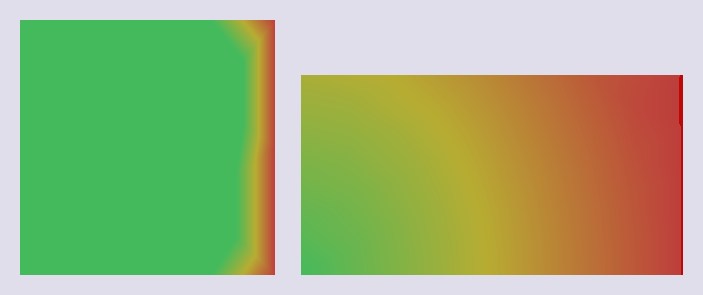
\includegraphics[width=.7\linewidth]{figures/static_analysis}
  \caption{Solution of the static analysis. Left: the initial
condition, right: the solution (deformation magnified 50 times)}
  \label{fig:smm:implicit:static_solution}
\end{figure}

\section{Dynamic Methods} \label{sect:smm:Dynamic_methods}

Different ways to solve the equations of motion are implemented in the
solid mechanics model.  The complete equations that should be solved
are:
\begin{equation}
\label{eqn:equation-motion}
\mat{M}\ddot{\vec{u}} +
\mat{C}\dot{\vec{u}} + \mat{K}\vec{u} = \vec{f}_{\st{ext}}~,
\end{equation}
where $\mat{M}$, $\mat{C}$ and $\mat{K}$ are the mass,
damping and stiffness matrices, respectively.

In the previous section, it has already been discussed how to solve this
equation in the static case, where $\ddot{\vec{u}} = \dot{\vec{u}} = 0$.  Here
the method to solve this equation in the general case will be presented.  For
this purpose, a time discretization has to be specified.  The most common
discretization method in solid mechanics is the Newmark-$\beta$ method, which is
also the default in \akantu.

For the Newmark-$\beta$ method, (\ref{eqn:equation-motion}) becomes a
system of three equations (see \cite{curnier92a} \cite{hughes-83a} for
more details):
\begin{align}
\mat{M} \ddot{\vec{u}}_{n+1} + \mat{C}\dot{\vec{u}}_{n+1} + \mat{K} \vec{u}_{n+1} &={\vec{f}_{\st{ext}}}_{\, n+1}
\label{eqn:equation-motion-discret} \\
\vec{u}_{n+1} &=\vec{u}_{n} + \left(1 - \alpha\right) \Delta t \dot{\vec{u}}_{n} +
\alpha \Delta t \dot{\vec{u}}_{n+1} + \left(\frac{1}{2} -
\alpha\right) \Delta t^2
\ddot{\vec{u}}_{n} \label{eqn:finite-difference-1}\\
\dot{\vec{u}}_{n+1} &= \dot{\vec{u}}_{n} + \left(1 - \beta\right)
\Delta t \ddot{\vec{u}}_{n} + \beta \Delta t
\ddot{\vec{u}}_{n+1} \label{eqn:finite-difference-2}
\end{align}

In these new equations, $\ddot{\vec{u}}_{n}$, $\dot{\vec{u}}_{n}$ and
$\vec{u}_{n}$ are the approximations of $\ddot{\vec{u}}(t_n)$,
$\dot{\vec{u}}(t_n)$ and $\vec{u}(t_n)$.
Equation~(\ref{eqn:equation-motion-discret}) is the equation of motion
discretized in space (finite-element discretization), and equations
(\ref{eqn:finite-difference-1}) and (\ref{eqn:finite-difference-2})
are discretized in both space and time (Newmark discretization).  The
$\alpha$ and $\beta$ parameters determine the stability and the
accuracy of the algorithm. Classical values for $\alpha$ and $\beta$
are usually $\beta = 1/2$ for no numerical damping and $0 < \alpha <
1/2$.

\begin{center}
  \begin{tabular}{cll}
    \toprule
    $\alpha$ & Method ($\beta = 1/2$) & Type\\
    \midrule
    $0$ & central difference & explicit\\
    $1/6$ & Fox-Goodwin (royal road) &implicit\\
    $1/3$ & Linear acceleration &implicit\\
    $1/2$ & Average acceleration (trapezoidal rule)& implicit\\
    \bottomrule
  \end{tabular}
\end{center}

The solution of this system of equations,
(\ref{eqn:equation-motion-discret})-(\ref{eqn:finite-difference-2}) is
split into a predictor and a corrector system of equations.  Moreover,
in the case of a non-linear equations, an iterative algorithm such as
the Newton-Raphson method is applied. The system of equations can be
written as:

\begin{enumerate}
\item \textit{Predictor:}
\begin{align}
  \vec{u}_{n+1}^{0} &= \vec{u}_{n} + \Delta t
  \dot{\vec{u}}_{n} + \frac{\Delta t^2}{2} \ddot{\vec{u}}_{n} \\
  \dot{\vec{u}}_{n+1}^{0} &= \dot{\vec{u}}_{n} + \Delta t
  \ddot{\vec{u}}_{n} \\
  \ddot{\vec{u}}_{n+1}^{0} &= \ddot{\vec{u}}_{n}
\end{align}

\item \textit{Solve:}
\begin{align}
  \left(c \mat{M} + d \mat{C} + e \mat{K}_{n+1}^i\right)
  \vec{w} = {\vec{f}_{\st{ext}}}_{\,n+1} - {\vec{f}_{\st{int}}}_{\,n+1}^i -
  \mat{C} \dot{\vec{u}}_{n+1}^i - \mat{M} \ddot{\vec{u}}_{n+1}^i = \vec{r}_{n+1}^i
\end{align}

\item \textit{Corrector:}
\begin{align}
  \ddot{\vec{u}}_{n+1}^{i+1} &= \ddot{\vec{u}}_{n+1}^{i} +c \vec{w} \\
  \dot{\vec{u}}_{n+1}^{i+1} &= \dot{\vec{u}}_{n+1}^{i} + d\vec{w} \\
  \vec{u}_{n+1}^{i+1} &= \vec{u}_{n+1}^{i} + e \vec{w}
\end{align}
\end{enumerate}

where $i$ is the Newton-Raphson iteration counter and $c$, $d$ and $e$
are parameters depending on the method used to solve the equations

\begin{center}
  \begin{tabular}{lcccc}
    \toprule
    & $\vec{w}$ & $e$ & $d$ & $c$\\
    \midrule
    in acceleration &$ \delta\ddot{\vec{u}}$ & $\alpha \beta\Delta t^2$ &$\beta \Delta t$ &$1$\\
    in velocity & $ \delta\dot{\vec{u}}$& $\frac{1}{\beta} \Delta t$ & $1$ & $\alpha\Delta t$\\
    in displacement &$\delta\vec{u}$ & $ 1$ & $\frac{1}{\alpha} \Delta t$ & $\frac{1}{\alpha \beta} \Delta t^2$\\
    \bottomrule
  \end{tabular}
\end{center}

% \note{If you want to use the implicit solver \akantu should be compiled at
% least with one sparse matrix solver such as Mumps\cite{mumps}.}


\subsection{Implicit Time Integration}
To solve a problem with an implicit time integration scheme, first a
\code{SolidMechanicsModel} object has to be created and initialized.
Then the initial and boundary conditions have to be set.  Everything
is similar to the example in the static case
(Section~\ref{sect:smm:static}), however, in this case the implicit
dynamic scheme is selected at the initialization of the model.

\begin{cpp}
SolidMechanicsModel model(mesh);
model.initFull(SolidMechanicsModelOptions(_implicit_dynamic));
/*Boundary conditions see Section~%\ref{sect:smm:boundary}% */
\end{cpp}
Because a dynamic simulation is conducted, an integration time step
$\Delta t$ has to be specified. In the case of implicit simulations,
\akantu implements a trapezoidal rule by default.  That is to say
$\alpha = 1/2$ and $\beta = 1/2$ which is unconditionally
stable. Therefore the value of the time step can be chosen arbitrarily
within reason.  \index{SolidMechanicsModel!setTimeStep}
\begin{cpp}
model.setTimeStep(time_step);
\end{cpp}
Since the system has to be solved for a given amount of time steps, the
method \code{solveStep()}, (which has already been used in the static
example in Section~\ref{sect:smm:static}), is called inside a time
loop:
\begin{cpp}
/// time loop
Real time = 0.;
for (UInt s = 1; time <max_time; ++s, time += time_step) {
  model.solveStep<_scm_newton_raphson_tangent_modified,_scc_increment>(1e-12, 100);
}
\end{cpp}
An example of solid mechanics with an implicit time integration scheme
is presented in
\shellcode{\examplesdir/implicit/implicit\_dynamic.cc}.  This example
consists of a 3D beam of
$\SI{10}{\metre}\,\times\,\SI{1}{\metre}\,\times\,\SI{1}{\metre}$
blocked on one side and is on a roller on the other side.  A constant
force of \SI{5}{\kilo\newton} is applied in its middle.
Figure~\ref{fig:smm:implicit:dynamic} presents the geometry of this
case. The material used is a fictitious linear elastic material with a
density of \SI{1000}{\kilo\gram\per\cubic\metre}, a Young's Modulus of
\SI{120}{\mega\pascal} and Poisson's ratio of $0.3$. These values
were chosen to simplify the analytical solution.

An approximation of the dynamic response of the middle point of the
beam is given by:
\begin{equation}
  \label{eqn:smm:implicit}
  u\left(\frac{L}{2}, t\right)
  = \frac{1}{\pi^4} \left(1 - cos\left(\pi^2 t\right) +
    \frac{1}{81}\left(1 - cos\left(3^2 \pi^2 t\right)\right) +
    \frac{1}{625}\left(1 - cos\left(5^2 \pi^2 t\right)\right)\right)
\end{equation}

\begin{figure}[!htb]
  \centering
  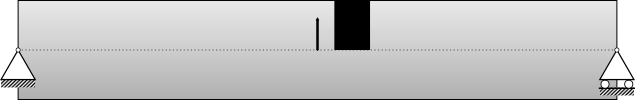
\includegraphics[scale=.6]{figures/implicit_dynamic}
  \caption{Numerical setup}
  \label{fig:smm:implicit:dynamic}
\end{figure}

Figure \ref{fig:smm:implicit:dynamic_solution} presents the deformed
beam at 3 different times during the simulation: time steps 0, 1000 and
2000.

\begin{figure}[!htb]
  \centering
  \setlength{\unitlength}{0.1\textwidth}
  \begin{tikzpicture}
    \node[above right] (img) at (0,0)
    {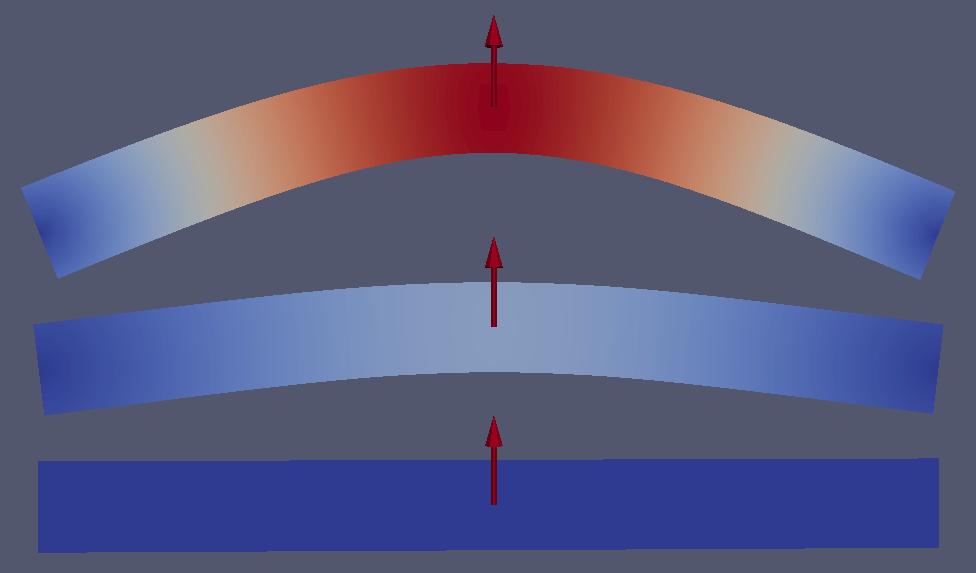
\includegraphics[width=.6\linewidth]{figures/dynamic_analysis}};
    \node[left] at (0pt,20pt) {$0$}; \node[left] at (0pt,60pt) {$1000$};
    \node[left] at (0pt,100pt) {$2000$};
  \end{tikzpicture}

  \caption{Deformed beam at 3 different times (displacement are
    magnified by a factor 10).}
  \label{fig:smm:implicit:dynamic_solution}
\end{figure}

\subsection{Explicit Time Integration}
\label{ssect:smm:expl-time-integr}

The explicit dynamic time integration scheme is based on the
Newmark-$\beta$ scheme with $\alpha=0$ (see equations
\ref{eqn:equation-motion-discret}-\ref{eqn:finite-difference-2}).  In
\akantu, $\beta$ is defaults to $\beta=1/2$, see section
\ref{sect:smm:Dynamic_methods}.

The initialization of the simulation is similar to the static and
implicit dynamic version.  The model is created from the
\code{SolidMechanicsModel} class.  In the initialization, the explicit
scheme is selected using the \code{\_explicit\_lumped\_mass} constant.

\begin{cpp}
SolidMechanicsModel model(mesh);
model.initFull(SolidMechanicsModelOptions(_explicit_lumped_mass));
\end{cpp}
\index{SolidMechanicsModel!initFull}
\note{Writing \code{model.initFull()} or \code{model.initFull(SolidMechanicsModelOptions());} is
equivalent to use the \code{\_explicit\_lumped\_mass} keyword, as this
is the default case.}

The explicit time integration scheme implemented in \akantu uses a
lumped mass matrix $\mat{M}$ (reducing the computational cost). This
matrix is assembled by distributing the mass of each element onto its
nodes. The resulting $\mat{M}$ is therefore a diagonal matrix stored
in the \textbf{mass} vector of the model.

The explicit integration scheme is conditionally stable. The time step
has to be smaller than the stable time step which is obtained in
\akantu as follows:

\begin{cpp}
critical_time_step = model.getStableTimeStep();
\end{cpp} \index{SolidMechanicsModel!StableTimeStep}

The stable time  step corresponds to the time the fastest wave (the compressive
wave) needs to travel the characteristic length of the mesh:
\begin{equation}
\label{eqn:smm:explicit:stabletime}
\Delta t_{\st{crit}} = \frac{\Delta x}{c}
\end{equation}
where $\Delta x$ is a characteristic length (\eg the inradius in the case of
linear triangle element) and $c$ is the celerity of the fastest wave in the
material. It is generally the compressive wave of celerity
$c = \sqrt{\frac{2 \mu + \lambda}{\rho}}$, $\mu$ and $\lambda$ are the first and
second Lame's coefficients and $\rho$ is the density. However, it is recommended
to impose a time step that is smaller than the stable time step, for instance,
by multiplying the stable time step by a safety factor smaller than one.

\begin{cpp}
const Real safety_time_factor = 0.8;
Real applied_time_step = critical_time_step * safety_time_factor;
model.setTimeStep(applied_time_step);
\end{cpp}
\index{SolidMechanicsModel!setTimeStep} The initial displacement and
velocity fields are, by default, equal to zero if not given
specifically by the user (see \ref{sect:smm:initial_condition}).

Like in implicit dynamics, a time loop is used in which the
displacement, velocity and acceleration fields are updated at each
time step. The values of these fields are obtained from the
Newmark$-\beta$ equations with $\beta=1/2$ and $\alpha=0$. In \akantu
these computations at each time step are invoked by calling the
function \code{solveStep}:
\begin{cpp}
for (UInt s = 1; (s-1)*applied_time_step < total_time; ++s) {
  model.solveStep();
}
\end{cpp} \index{SolidMechanicsModel!solveStep}
The method
\code{solveStep} wraps the four following functions:
\begin{itemize}
\item \code{model.explicitPred()} allows to compute the displacement
  field at $t+1$ and a part of the velocity field at $t+1$, denoted by
  $\vec{\dot{u}^{\st{p}}}_{n+1}$, which will be used later in the method
  \code{model.explicitCorr()}. The equations are:
  \begin{align}
    \vec{u}_{n+1} &= \vec{u}_{n} + \Delta t
    \vec{\dot{u}}_{n} + \frac{\Delta t^2}{2} \vec{\ddot{u}}_{n}\\
    \vec{\dot{u}^{\st{p}}}_{n+1} &= \vec{\dot{u}}_{n} + \Delta t
    \vec{\ddot{u}}_{n}
    \label{eqn:smm:explicit:onehalfvelocity}
  \end{align}

\item \code{model.updateResidual()} and
  \code{model.updateAcceleration()} compute the acceleration increment
  $\delta \vec{\ddot{u}}$:
  \begin{equation}
    \left(\mat{M} + \frac{1}{2} \Delta t \mat{C}\right)
    \delta \vec{\ddot{u}} = \vec{f_{\st{ext}}} - \vec{f}_{\st{int}\, n+1}
    - \mat{C} \vec{\dot{u}}_{n} - \mat{M} \vec{\ddot{u}}_{n}
  \end{equation}

  \note{The internal force $\vec{f}_{\st{int}\, n+1}$ is computed from
    the displacement $\vec{u}_{n+1}$ based on the constitutive law.}

\item \code{model.explicitCorr()} computes the velocity and
  acceleration fields at $t+1$:
  \begin{align}
    \vec{\dot{u}}_{n+1} &= \vec{\dot{u}^{\st{p}}}_{n+1} + \frac{\Delta t}{2}
    \delta \vec{\ddot{u}} \\ \vec{\ddot{u}}_{n+1} &=
    \vec{\ddot{u}}_{n} + \delta \vec{\ddot{u}}
  \end{align}
\end{itemize}

The use of an explicit time integration scheme is illustrated by the
example:\par
\noindent \shellcode{\examplesdir/explicit/explicit\_dynamic.cc}\par
\noindent This example models the propagation of a wave in a steel beam. The
beam and the applied displacement in the $x$ direction are shown in
Figure~\ref{fig:smm:explicit}.

\begin{figure}[!htb] \centering
  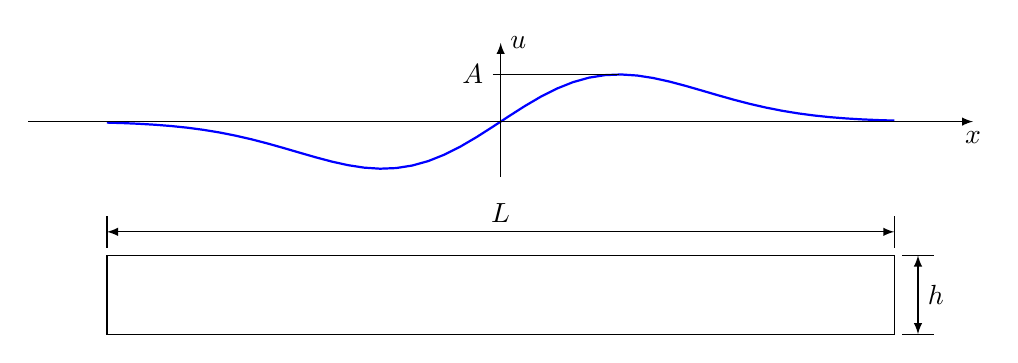
\begin{tikzpicture}
    \coordinate (c) at (0,2);
    \draw[shift={(c)},thick, color=blue] plot [id=x, domain=-5:5, samples=50] ({\x, {(40 * sin(0.1*pi*3*\x) * exp(- (0.1*pi*3*\x)*(0.1*pi*3*\x) / 4))}});
    \draw[shift={(c)},-latex] (-6,0) -- (6,0) node[right, below] {$x$};
    \draw[shift={(c)},-latex] (0,-0.7) -- (0,1) node[right] {$u$};
    \draw[shift={(c)}] (-0.1,0.6) node[left] {$A$}-- (1.5,0.6);

    \coordinate (l) at (0,0.6);
    \draw[shift={(0,-0.7)}] (-5, 0) -- (5,0) -- (5, 1) -- (-5, 1) -- cycle;
    \draw[shift={(l)}, latex-latex] (-5,0)-- (5,0) node [midway, above] {$L$};
    \draw[shift={(l)}] (5,0.2)-- (5,-0.2);
    \draw[shift={(l)}] (-5,0.2)-- (-5,-0.2);

    \coordinate (h) at (5.3,-0.7);
    \draw[shift={(h)}, latex-latex] (0,0)-- (0,1) node [midway, right] {$h$};
    \draw[shift={(h)}] (-0.2,1)-- (0.2,1);
    \draw[shift={(h)}] (-0.2,0)-- (0.2,0);
  \end{tikzpicture}

  \caption{Numerical setup \label{fig:smm:explicit}}
\end{figure}

The length and height of the beam are $L=\SI{10}{\metre}$ and
$h = \SI{1}{\metre}$, respectively.  The material is linear elastic,
homogeneous and isotropic (density:
\SI{7800}{\kilo\gram\per\cubic\metre}, Young's modulus:
\SI{210}{\giga\pascal} and Poisson's ratio: $0.3$).  The imposed
displacement follow a Gaussian function with a maximum amplitude of $A = \SI{0.01}{\meter}$. The
potential, kinetic and total energies are computed.  The safety factor
is equal to $0.8$.

\section{Constitutive Laws \label{sect:smm:CL}}\index{Material}
In order to compute an element's response to deformation, one needs to
use an appropriate constitutive relationship. The constitutive law is
used to compute the element's stresses from the element's strains.

In the finite-element discretization, the constitutive formulation is
applied to every quadrature point of each element. When the implicit
formulation is used, the tangent matrix has to be computed.

The chosen materials for the simulation have to be specified in the
mesh file or, as an alternative, they can be assigned using the
\code{element\_material} vector.  For every material assigned to the
problem one has to specify the material characteristics (constitutive
behavior and material properties) using the text input file (see \ref{sect:io:material}).\\
In order to conveniently store values at each quadrature in a material
point \akantu provides a special data structure, the
\code{InternalField}. The internal fields are inheriting from the
\code{ElementTypeMapArray}.  Furthermore, it provides several functions for
initialization, auto-resizing and auto removal of quadrature points.

Sometimes it is also desired to generate random distributions of
internal parameters. An example might be the critical stress at which the
material fails. To generate such a field, in the text input file,
a random quantity needs be added to the base value:
\begin{cpp}
  sigma_c = $base$
  sigma_c = $base$ uniform [$min$, $max$]
  sigma_c = $base$ weibull [$\lambda$, $m$]
\end{cpp}

All parameters are real numbers. For the uniform distribution, minimum
and maximum values have to be specified.
Random parameters are defined as a $base$ value to which we add a random number
that follows the chosen distribution.

The
\href{http://en.wikipedia.org/wiki/Uniform\_distribution\_(continuous)}{\emph{Uniform}}
distribution is gives a random values between in $[min, max)$. The
\href{http://en.wikipedia.org/wiki/Weibull\_distribution}{\emph{Weibull}}
distribution is characterized by the following cumulative distribution
function:
\begin{equation}
  F(x) = 1- e^{-\left({x/\lambda}\right)^m}
\end{equation}
which depends on  $m$ and $\lambda$, which are the shape parameter and the scale
parameter. These random distributions are different each time the code
is executed. In order to obtain always the same one, it possible to
manually set the \emph{seed} that is the number from which these
pseudo-random distributions are created. This can be done by adding
the following line to the input file \emph{outside} the material
parameters environments:
\begin{cpp}
  seed = 1.0
\end{cpp}
where the value 1 can be substituted with any number. Currently
\akantu is can reproduce always the same distribution when the seed is
specified \emph{only} in serial.

The following sections describe the constitutive models implemented in
\akantu. In Appendix~\ref{app:material-parameters} a summary of the
parameters for all materials of \akantu is provided.


\subsection{Elasticity}\index{Material!Elastic}

The elastic law is a commonly used constitutive relationship that can be used
for a wide range of engineering materials (\eg metals, concrete, rock, wood,
glass, rubber, etc.) provided that the strains remain small (\ie small
deformation and stress lower than yield strength).

The elastic laws are often expressed as $\mat{\sigma} =
\mat{C}:\mat{\varepsilon}$ with where $\mat{\sigma}$ is the Cauchy stress tensor,
$\mat{\varepsilon}$ represents the infinitesimal strain tensor and $\mat{C}$ is the
elastic modulus tensor.

\subsubsection{Linear isotropic\matlabel{ssect:smm:linear-elastic-isotropic}}

The linear isotropic elastic behavior is described by Hooke's law, which states
that the stress is linearly proportional to the applied strain (material behaves
like an ideal spring), as illustrated in Figure~\ref{fig:smm:cl:elastic}.
\begin{figure}[!htb]
  \begin{center}

    \subfloat[]{
      \begin{tikzpicture}
	\draw[thick,latex-latex] (0,5) node[left] {$\sigma$} |- (5,0) node (x) [right, below] {$\varepsilon$};
	\draw[thin] (1.5,1.5) -- (2.5,1.5) -- (2.5,2.5) node [midway, right] {E};
	\draw[very thick,color=red] (0,0) -- (4,4);
	\draw[very thick,latex-latex,color=red] (1,1) -- (3,3);
      \end{tikzpicture}
      \label{fig:smm:cl:elastic:stress_strain} }
    \hspace{0.05\textwidth} \subfloat[]{
      \raisebox{0.125\textwidth}{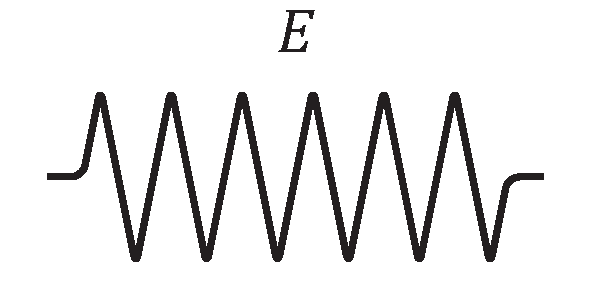
\includegraphics[width=0.25\textwidth,keepaspectratio=true]{figures/hooke_law.pdf}}
      \label{fig:smm:cl:elastic:hooke} }
    \caption{(a) Stress-strain curve for elastic material and (b)
      schematic representation of Hooke's law, denoted as a spring.}
    \label{fig:smm:cl:elastic}
  \end{center}
\end{figure}
The equation that relates the strains to the
displacements is: % First the strain is computed (at every gauss
point) from the displacements as follows:
\begin{equation}
  \label{eqn:smm:strain_inf}
  \mat{\varepsilon} =
  \frac{1}{2} \left[ \nabla_0 \vec{u}+\nabla_0 \vec{u}^T \right]
\end{equation}
where $\mat{\varepsilon}$ represents the infinitesimal strain tensor,
$\nabla_{0}\vec{u}$ the displacement gradient
tensor according to the initial configuration. The constitutive equation
for isotropic homogeneous media can be expressed as:
\begin{equation}
  \label{eqn:smm:material:constitutive_elastic}
  \mat{\sigma } =\lambda\mathrm{tr}(\mat{\varepsilon})\mat{I}+2 \mu\mat{\varepsilon}
\end{equation}
where $\mat{\sigma}$ is the Cauchy stress tensor
($\lambda$ and $\mu$ are the the first and second Lame's
coefficients).

In Voigt notation this correspond to
\begin{align}
  \left[\begin{array}{c}
      \sigma_{11}\\
      \sigma_{22}\\
      \sigma_{33}\\
      \sigma_{23}\\
      \sigma_{13}\\
      \sigma_{12}\\
    \end{array}\right]
  &= \frac{E}{(1+\nu)(1-2\nu)}\left[
    \begin{array}{cccccc}
      1-\nu & \nu   & \nu   & 0 & 0 & 0\\
      \nu   & 1-\nu & \nu   & 0 & 0 & 0\\
      \nu   & \nu   & 1-\nu & 0 & 0 & 0\\
      0     &  0    &  0    & \frac{1-2\nu}{2} & 0 & 0 \\
      0     &  0    &  0    & 0 & \frac{1-2\nu}{2} & 0 \\
      0     &  0    &  0    & 0 & 0 & \frac{1-2\nu}{2} \\
    \end{array}\right]
  \left[\begin{array}{c}
      \varepsilon_{11}\\
      \varepsilon_{22}\\
      \varepsilon_{33}\\
      2\varepsilon_{23}\\
      2\varepsilon_{13}\\
      2\varepsilon_{12}\\
    \end{array}\right]
\end{align}

\subsubsection{Linear anisotropic\matlabel{ssect:smm:linear-elastic-anisotropic}}
This formulation is not sufficient to represent all elastic material
behavior. Some materials have characteristic orientation that have to be taken
into account. To represent this anisotropy a more general stress-strain law has
to be used. For this we define the elastic modulus tensor as follow:

\begin{align}
  \left[\begin{array}{c}
      \sigma_{11}\\
      \sigma_{22}\\
      \sigma_{33}\\
      \sigma_{23}\\
      \sigma_{13}\\
      \sigma_{12}\\
    \end{array}\right]
  &= \left[
    \begin{array}{cccccc}
      c_{11} & c_{12} & c_{13} & c_{14} & c_{15} & c_{16}\\
      c_{21} & c_{22} & c_{23} & c_{24} & c_{25} & c_{26}\\
      c_{31} & c_{32} & c_{33} & c_{34} & c_{35} & c_{36}\\
      c_{41} & c_{42} & c_{43} & c_{44} & c_{45} & c_{46}\\
      c_{51} & c_{52} & c_{53} & c_{54} & c_{55} & c_{56}\\
      c_{61} & c_{62} & c_{63} & c_{64} & c_{65} & c_{66}\\
    \end{array}\right]
  \left[\begin{array}{c}
      \varepsilon_{11}\\
      \varepsilon_{22}\\
      \varepsilon_{33}\\
      2\varepsilon_{23}\\
      2\varepsilon_{13}\\
      2\varepsilon_{12}\\
    \end{array}\right]
\end{align}

\begin{figure}[h]
  \centering
  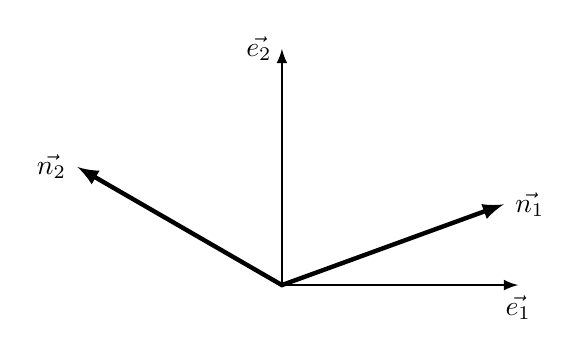
\begin{tikzpicture}
    \draw[thick,latex-latex] (90:3) node[left] {$\vec{e_2}$} |- (0:3) node [right, below] {$\vec{e_1}$};
    \draw[ultra thick,latex-latex] (150:3) node[left] {$\vec{n_2}$} -- (0,0) -- (20:3) node [right] {$\vec{n_1}$};
  \end{tikzpicture}
  \caption{Material basis}
\end{figure}

To simplify the writing of input files the \mat{C} tensor is expressed in the
material basis. And this basis as to be given too. This basis $\Omega_{\st{mat}}
= \{\vec{n_1}, \vec{n_2}, \vec{n_3}\}$ is used to define the rotation $R_{ij} =
\vec{n_j} . \vec{e_i}$. And $\mat{C}$ can be rotated in the global basis $\Omega
= \{\vec{e_1}, \vec{e_2}, \vec{e_3}\}$ as follow:


\begin{align}
\mat{C}_{\Omega} &= \mat{R}_1 \mat{C}_{\Omega_{\st{mat}}} \mat{R}_2\\
\mat{R}_1  &= \left[
  \begin{array}{cccccc}
    R_{11} R_{11} & R_{12} R_{12} & R_{13} R_{13} & R_{12} R_{13} & R_{11} R_{13} & R_{11} R_{12}\\
    R_{21} R_{21} & R_{22} R_{22} & R_{23} R_{23} & R_{22} R_{23} & R_{21} R_{23} & R_{21} R_{22}\\
    R_{31} R_{31} & R_{32} R_{32} & R_{33} R_{33} & R_{32} R_{33} & R_{31} R_{33} & R_{31} R_{32}\\
    R_{21} R_{31} & R_{22} R_{32} & R_{23} R_{33} & R_{22} R_{33} & R_{21} R_{33} & R_{21} R_{32}\\
    R_{11} R_{31} & R_{12} R_{32} & R_{13} R_{33} & R_{12} R_{33} & R_{11} R_{33} & R_{11} R_{32}\\
    R_{11} R_{21} & R_{12} R_{22} & R_{13} R_{23} & R_{12} R_{23} & R_{11} R_{23} & R_{11} R_{22}\\
  \end{array}\right]\\
\mat{R}_2  &= \left[
  \begin{array}{cccccc}
    R_{11} R_{11} & R_{21} R_{21} & R_{31} R_{31} & R_{21} R_{31} & R_{11} R_{31} & R_{11} R_{21}\\
    R_{12} R_{12} & R_{22} R_{22} & R_{32} R_{32} & R_{22} R_{32} & R_{12} R_{32} & R_{12} R_{22}\\
    R_{13} R_{13} & R_{23} R_{23} & R_{33} R_{33} & R_{23} R_{33} & R_{13} R_{33} & R_{13} R_{23}\\
    R_{12} R_{13} & R_{22} R_{23} & R_{32} R_{33} & R_{22} R_{33} & R_{12} R_{33} & R_{12} R_{23}\\
    R_{11} R_{13} & R_{21} R_{23} & R_{31} R_{33} & R_{21} R_{33} & R_{11} R_{33} & R_{11} R_{23}\\
    R_{11} R_{12} & R_{21} R_{22} & R_{31} R_{32} & R_{21} R_{32} & R_{11} R_{32} & R_{11} R_{22}\\
  \end{array}\right]\\
\end{align}

\subsubsection{Linear orthotropic\matlabel{ssect:smm:linear-elastic-orthotropic}}

A particular case of anisotropy is when the material basis is orthogonal in which case the elastic modulus tensor can be simplified and rewritten in terms of 9 independents material parameters.

\begin{align}
  \left[\begin{array}{c}
      \sigma_{11}\\
      \sigma_{22}\\
      \sigma_{33}\\
      \sigma_{23}\\
      \sigma_{13}\\
      \sigma_{12}\\
    \end{array}\right]
  &= \left[
    \begin{array}{cccccc}
      c_{11} & c_{12} & c_{13} &   0   &   0   &   0  \\
            & c_{22} & c_{23} &   0   &   0   &   0  \\
            &       & c_{33} &   0   &   0   &   0  \\
            &       &       & c_{44} &   0   &   0  \\
            &  \multicolumn{2}{l}{\text{sym.}}       &       & c_{55} &   0  \\
            &       &       &       &       & c_{66}\\
    \end{array}\right]
  \left[\begin{array}{c}
      \varepsilon_{11}\\
      \varepsilon_{22}\\
      \varepsilon_{33}\\
      2\varepsilon_{23}\\
      2\varepsilon_{13}\\
      2\varepsilon_{12}\\
    \end{array}\right]
\end{align}

\begin{align}
  c_{11} &= E_1 (1 - \nu_{23}\nu_{32})\Gamma \qquad c_{22} = E_2 (1 - \nu_{13}\nu_{31})\Gamma \qquad c_{33} = E_3 (1 - \nu_{12}\nu_{21})\Gamma\\
  c_{12} &= E_1 (\nu_{21} - \nu_{31}\nu_{23})\Gamma = E_2 (\nu_{12} - \nu_{32}\nu_{13})\Gamma\\
  c_{13} &= E_1 (\nu_{31} - \nu_{21}\nu_{32})\Gamma = E_2 (\nu_{13} - \nu_{21}\nu_{23})\Gamma\\
  c_{23} &= E_2 (\nu_{32} - \nu_{12}\nu_{31})\Gamma = E_3 (\nu_{23} - \nu_{21}\nu_{13})\Gamma\\
  c_{44} &= \mu_{23} \qquad  c_{55} = \mu_{13} \qquad  c_{66} = \mu_{12} \\
  \Gamma &= \frac{1}{1 - \nu_{12} \nu_{21} - \nu_{13} \nu_{31} - \nu_{32} \nu_{23} - 2 \nu_{21} \nu_{32} \nu_{13}}
\end{align}

The Poisson ratios follow the rule $\nu_{ij} = \nu_{ji} E_i / E_j$.

\subsection{Neo-Hookean\matlabel{ssect:smm:cl:neohookean}}\index{Material!Neohookean}
The hyperelastic Neo-Hookean constitutive law results from an
extension of the linear elastic relationship (Hooke's Law) for large
deformation. Thus, the model predicts nonlinear stress-strain behavior
for bodies undergoing large deformations.

\begin{figure}[!htb]
  \begin{center}
    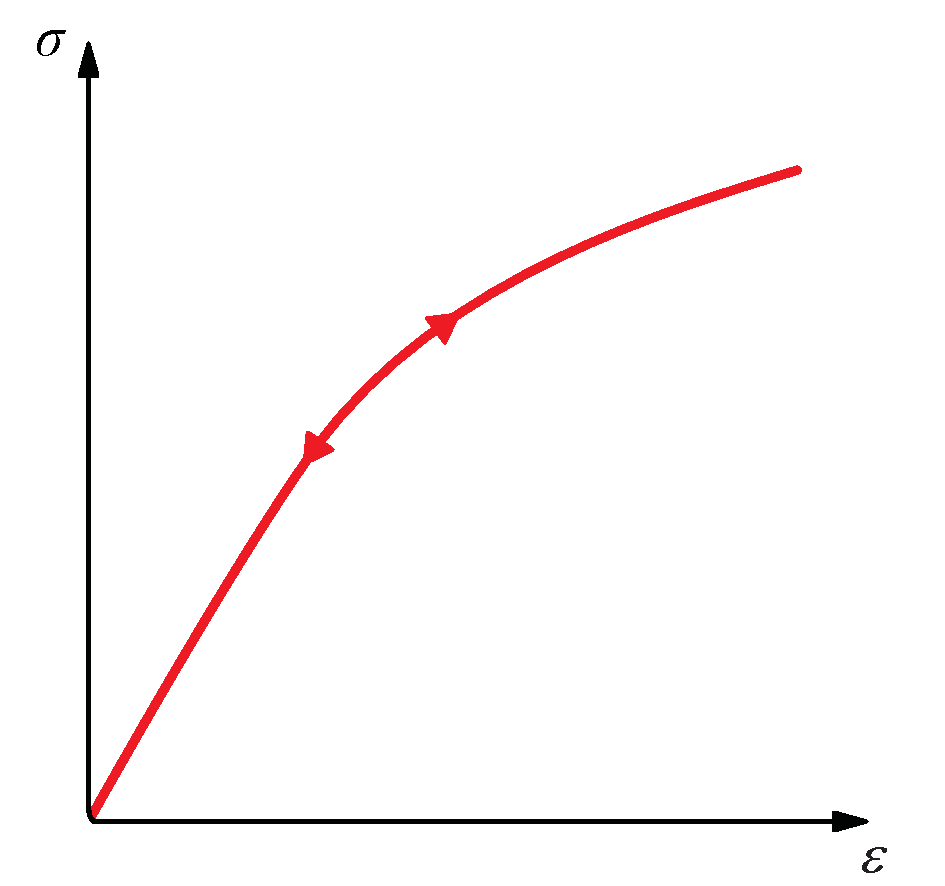
\includegraphics[width=0.4\textwidth,keepaspectratio=true]{figures/stress_strain_neo.pdf}
    \caption{Neo-hookean Stress-strain curve.}
    \label{fig:smm:cl:neo_hookean}
  \end{center}
\end{figure}

As illustrated in Figure~\ref{fig:smm:cl:neo_hookean}, the behavior is initially
linear and the mechanical behavior is very close to the corresponding linear
elastic material. This constitutive relationship, which accounts for compressibility,
is a modified version of the one proposed by Ronald Rivlin \cite{Belytschko:2000}.

The strain energy stored in the material is given by:
\begin{equation}\label{eqn:smm:constitutive:neohookean_potential}
  \Psi(\mat{C}) = \frac{1}{2}\lambda_0\left(\ln J\right)^2-\mu_0\ln J+\frac{1}{2}
  \mu_0\left(\mathrm{tr}(\mat{C})-3\right)
\end{equation}
\noindent where $\lambda_0$ and $\mu_0$ are, respectively, Lam\'e's first parameter
and the shear modulus at the initial configuration. $J$ is the jacobian of the deformation
gradient ($\mat{F}=\nabla_{\!\!\vec{X}}\vec{x}$): $J=\text{det}(\mat{F})$. Finally $\mat{C}$ is the right Cauchy-Green
deformation tensor.

Since this kind of material is used for large deformation problems, a
finite deformation framework should be used. Therefore, the Cauchy
stress ($\mat{\sigma}$) should be computed through the second
Piola-Kirchhoff stress tensor $\mat{S}$:

\begin{equation}
  \mat{\sigma } = \frac{1}{J}\mat{F}\mat{S}\mat{F}^T
\end{equation}

Finally the second Piola-Kirchhoff stress tensor is given by:

\begin{equation}
  \mat{S}  = 2\frac{\partial\Psi}{\partial\mat{C}} = \lambda_0\ln J
  \mat{C}^{-1}+\mu_0\left(\mat{I}-\mat{C}^{-1}\right)
\end{equation}

The parameters to indicate in the material file are the same
as those for the elastic case: \code{E} (Young's modulus), \code{nu} (Poisson's
ratio).


\subsection{Visco-Elasticity\matlabel{ssect:smm:cl:sls}}
% Standard Solid rheological model, see [] J.C. Simo, T.J.R. Hughes,
% "Computational Inelasticity", Springer (1998), see Sections 10.2 and 10.3
Visco-elasticity is characterized by strain rate dependent
behavior. Moreover, when such a material undergoes a deformation it
dissipates energy. This dissipation results in a hysteresis loop in
the stress-strain curve at every loading cycle (see
Figure~\ref{fig:smm:cl:visco-elastic:hyst}). In principle, it can be
applied to many materials, since all materials exhibit a visco-elastic
behavior if subjected to particular conditions (such as high
temperatures).
\begin{figure}[!htb]
  \begin{center}

    \subfloat[]{
      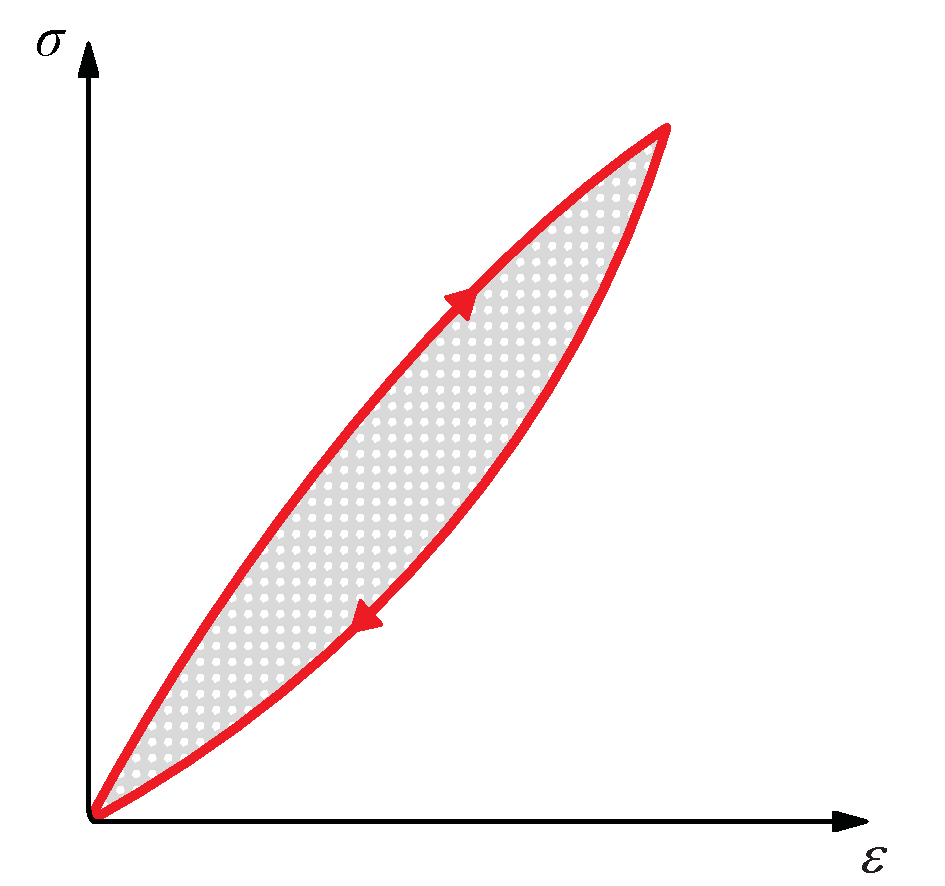
\includegraphics[width=0.4\textwidth,keepaspectratio=true]{figures/stress_strain_visco.pdf}
      \label{fig:smm:cl:visco-elastic:hyst}
    }
    \hspace{0.05\textwidth}
    \subfloat[]{
      \raisebox{0.025\textwidth}{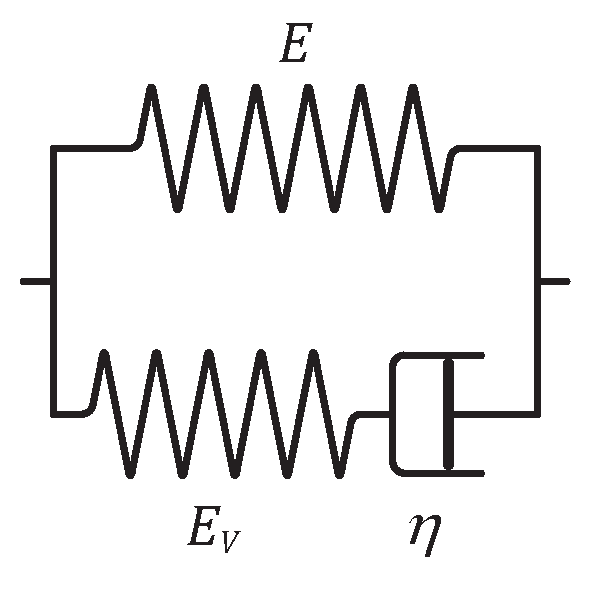
\includegraphics[width=0.3\textwidth,keepaspectratio=true]{figures/visco_elastic_law.pdf}}
      \label{fig:smm:cl:visco-elastic:model}
    }
    \caption{(a) Characteristic stress-strain behavior of a visco-elastic material with hysteresis loop and (b) schematic representation of the standard rheological linear solid visco-elastic model.}
    \label{fig:smm:cl:visco-elastic}
  \end{center}
\end{figure}
The standard rheological linear solid model (see Sections 10.2 and 10.3
of~\cite{simo92}) has been implemented in \akantu. This model results from the
combination of a spring mounted in parallel with a spring and a dashpot
connected in series, as illustrated in
Figure~\ref{fig:smm:cl:visco-elastic:model}. The advantage of this model is that
it allows to account for creep or stress relaxation. The equation that relates
the stress to the strain is (in 1D):
\begin{equation}
  \frac{d\varepsilon(t)}{dt} = \left ( E + E_V \right ) ^ {-1} \cdot \left [ \frac{d\sigma(t)}{dt} + \frac{E_V}{\eta}\sigma(t) - \frac{EE_V}{\eta}\varepsilon(t) \right ]
\end{equation}
where $\eta$ is the viscosity. The equilibrium condition is unique and
is attained in the limit, as $t \to \infty $. At this stage, the
response is elastic and depends on the Young's modulus $E$.  The
mandatory parameters for the material file are the following:
\code{rho} (density), \code{E} (Young's modulus), \code{nu} (Poisson's
ratio), \code{Plane\_Stress} (if set to zero plane strain, otherwise
plane stress), \code{eta} (dashpot viscosity) and \code{Ev} (stiffness
of the viscous element).

Note that the current standard linear solid model is applied only on the deviatoric part of the strain tensor. The spheric part of the strain tensor affects the stress tensor like an linear elastic material.

\subsection{Small-Deformation Plasticity\matlabel{ssect:smm:cl:plastic}}\index{Material!Small-deformation Plasticity}
The small-deformation plasticity is a simple plasticity material
formulation which accounts for the additive decomposition of strain
into elastic and plastic strain components. This formulation is
applicable to infinitesimal deformation where the additive
decomposition of the strain is a valid approximation. In this
formulation, plastic strain is a shearing process where hydrostatic
stress has no contribution to plasticity and consequently plasticity
does not lead to volume change. Figure~\ref{fig:smm:cl:Lin-strain-hard}
shows the linear strain hardening elasto-plastic behavior according to
the additive decomposition of strain into the elastic and plastic
parts in infinitesimal deformation as
\begin{align}
  \mat{\varepsilon} &= \mat{\varepsilon}^e +\mat{\varepsilon}^p\\
  {\mat{\sigma}} &= 2G(\mat{\varepsilon}^e) + \lambda  \mathrm{tr}(\mat{\varepsilon}^e)\mat{I}
\end{align}

\begin{figure}[htp]
  \centering
  {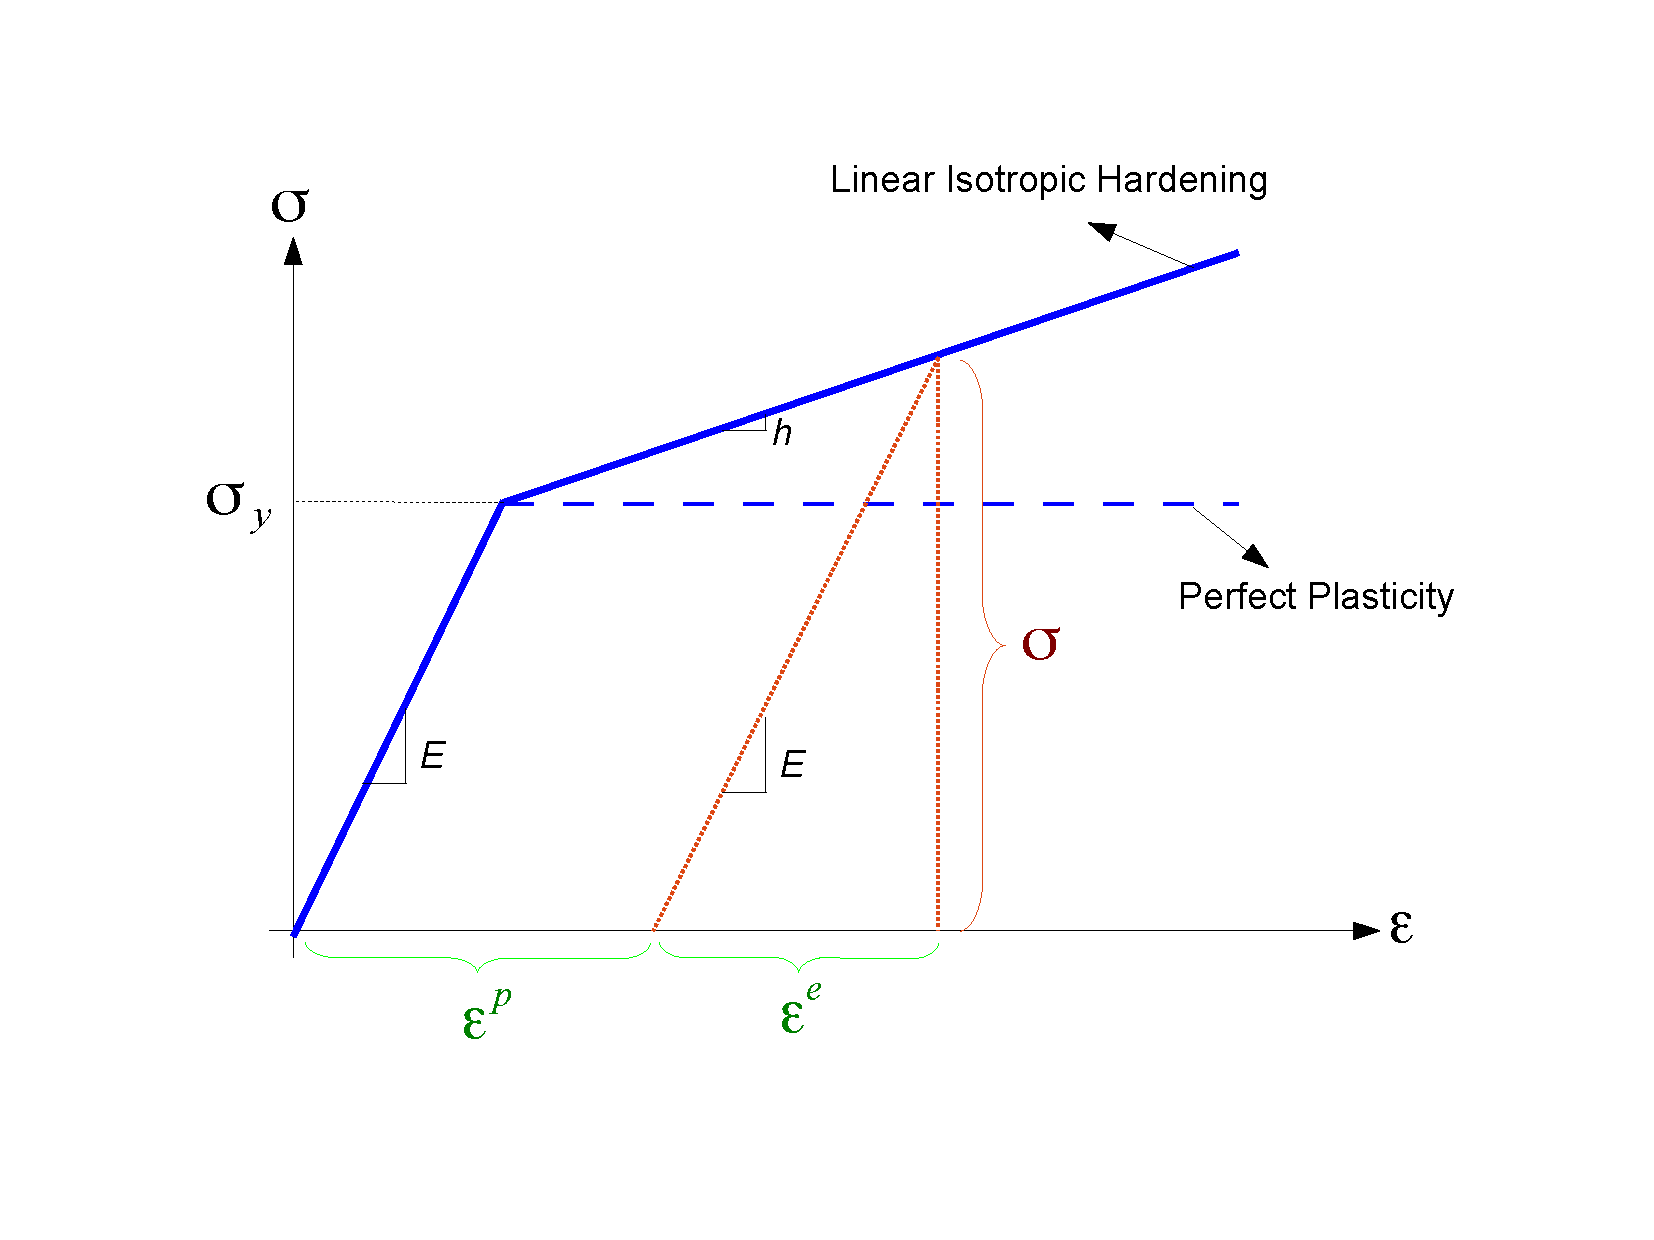
\includegraphics[scale=0.4, clip]{figures/isotropic_hardening_plasticity.pdf}}
  \caption{
    Stress-strain curve for the small-deformation plasticity with linear isotropic hardening.
  }
  \label{fig:smm:cl:Lin-strain-hard}
\end{figure}

\noindent In this class, the von Mises yield criterion is used. In the von Mises yield criterion, the yield is independent of the hydrostatic stress. Other yielding criteria such as Tresca and Gurson can be easily implemented in this class as well.

In the von Mises yield criterion, the hydrostatic stresses have no effect on the plasticity and consequently the yielding occurs when a critical elastic shear energy is achieved.
\begin{equation} \label{eqn:smm:constitutive:von Mises}
  f = \sigma_{\st{eff}} - \sigma_y = \left(\frac{3}{2} {\mat{\sigma}}^{\st{tr}} : {\mat{\sigma}}^{\st{tr}}\right)^\frac{1}{2}-\sigma_y (\mat{\varepsilon}^p)
\end{equation}
\begin{equation} \label{eqn:smm:constitutive:yielding}
  f < 0 \quad \textrm{Elastic deformation,} \qquad f = 0 \quad  \textrm{Plastic deformation}
\end{equation}
where $\sigma_y$ is the yield strength of the material which can be function of plastic strain in case of hardening type of materials and ${\mat{\sigma}}^{\st{tr}}$ is the deviatoric part of stress given by
\begin{equation} \label{eqn:smm:constitutive:deviatoric stress}
  {\mat{\sigma}}^{\st{tr}}=\mat{\sigma} - \frac{1}{3} \mathrm{tr}(\mat{\sigma}) \mat {I}
\end{equation}

After yielding $(f = 0)$, the normality hypothesis of plasticity determines the direction of plastic flow which is normal to the tangent to the yielding surface at the load point. Then, the tensorial form of the plastic constitutive equation using the von Mises yielding criterion (see equation 4.34) may be written as
\begin{equation} \label{eqn:smm:constitutive:plastic contitutive equation}
  \Delta {\mat{\varepsilon}}^p = \Delta p \frac {\partial{f}}{\partial{\mat \sigma}}=\frac{3}{2} \Delta p \frac{{\mat{\sigma}}^{\st{tr}}}{\sigma_{\st{eff}}}
\end{equation}

In these expressions, the direction of the plastic strain increment (or equivalently, plastic strain rate) is given by $\frac{{\mat{\sigma}}^{\st{tr}}}{\sigma_{\st{eff}}}$ while the magnitude is defined by the plastic multiplier $\Delta p$. This can be obtained using the \emph{consistency condition} which impose the requirement for the load point to remain on the yielding surface in the plastic regime.

Here, we summarize the implementation procedures for the
small-deformation plasticity with linear isotropic hardening:
\begin{enumerate}
\item Compute the trial stress:
  \begin{equation}
    {\mat{\sigma}}^{\st{tr}} = {\mat{\sigma}}_t + 2G\Delta \mat{\varepsilon} + \lambda \mathrm{tr}(\Delta \mat{\varepsilon})\mat{I}
  \end{equation}
\item Check the Yielding criteria:
  \begin{equation}
    f = (\frac{3}{2} {\mat{\sigma}}^{\st{tr}} : {\mat{\sigma}}^{\st{tr}})^{1/2}-\sigma_y (\mat{\varepsilon}^p)
  \end{equation}
\item Compute the Plastic multiplier:
  \begin{align}
    d \Delta p &= \frac{\sigma^{tr}_{eff} - 3G \Delta P^{(k)}- \sigma_y^{(k)}}{3G + h}\\
    \Delta p^{(k+1)} &= \Delta p^{(k)}+ d\Delta p\\
    \sigma_y^{(k+1)} &= (\sigma_y)_t+ h\Delta p
  \end{align}
\item Compute the plastic strain increment:
  \begin{equation}
    \Delta {\mat{\varepsilon}}^p = \frac{3}{2} \Delta p \frac{{\mat{\sigma}}^{\st{tr}}}{\sigma_{\st{eff}}}
  \end{equation}
\item Compute the stress increment:
  \begin{equation}
    {\Delta \mat{\sigma}} = 2G(\Delta \mat{\varepsilon}-\Delta \mat{\varepsilon}^p) + \lambda  \mathrm{tr}(\Delta \mat{\varepsilon}-\Delta \mat{\varepsilon}^p)\mat{I}
  \end{equation}
\item Update the variables:
  \begin{align}
    {\mat{\varepsilon^p}} &= {\mat{\varepsilon}}^p_t+{\Delta {\mat{\varepsilon}}^p}\\
    {\mat{\sigma}} &= {\mat{\sigma}}_t+{\Delta \mat{\sigma}}
  \end{align}
\end{enumerate}

We use an implicit integration technique called \emph{the radial
  return method} to obtain the plastic multiplier. This method has the
advantage of being unconditionally stable, however, the accuracy
remains dependent on the step size. The plastic parameters to indicate
in the material file are: \code{$\sigma_y$} (Yield stress) and
\code{h} (Hardening modulus). In addition, the elastic parameters need
to be defined as previously mentioned: \code{E} (Young's modulus),
\code{nu} (Poisson's ratio).

\subsection{Damage}

In the  simplified case of a  linear elastic and brittle  material, isotropic
damage can be represented by a scalar variable $d$, which varies from $0$ to $1$
for  no  damage  to  fully  broken  material  respectively.  The  stress-strain
relationship then becomes:
\begin{equation*}
  \mat{\sigma} = (1-d)\, \mat{C}:\mat{\varepsilon}
\end{equation*}

where  $\mat{\sigma}$,  $\mat{\varepsilon}$ are  the  Cauchy  stress and  strain
tensors, and $\mat{C}$ is the elastic stiffness tensor. This formulation relies
on the definition of an evolution law for the damage variable. In \akantu, many
possibilities exist and they are listed below.

\subsubsection{Marigo\matlabel{ssect:smm:cl:damage-marigo}}

This damage evolution law is energy based as defined by Marigo \cite{marigo81a,
  lemaitre96a}. It is an isotropic damage law.
\begin{align}
  Y &= \frac{1}{2}\mat{\varepsilon}:\mat{C}:\mat{\varepsilon}\\
  F &= Y - Y_d - S d\\
  d &= \left\{
    \begin{array}{l l}
      \mathrm{min}\left(\frac{Y-Y_d}{S},\;1\right) & \mathrm{if}\; F > 0\\
      \mathrm{unchanged} & \mathrm{otherwise}
    \end{array}
  \right.
\end{align}
In this formulation, $Y$ is the strain energy release rate, $Y_d$ the
rupture criterion and $S$ the damage energy.  The non-local version of
this damage evolution law is constructed by averaging the energy $Y$.

\subsubsection{Mazars\matlabel{ssect:smm:cl:damage-mazars}}

This law introduced by Mazars \cite{mazars84a} is a behavioral model to
represent damage evolution in concrete. This model does not rely on the computation of the tangent stiffness, the damage is directly evaluated from the strain.

The governing variable in this damage
law is the equivalent strain $\varepsilon_{\st{eq}} =
\sqrt{<\mat{\varepsilon}>_+:<\mat{\varepsilon}>_+}$, with $<.>_+$ the positive
part of the tensor. This part is defined in the principal coordinates (I, II, III) as $\varepsilon_{\st{eq}} =
\sqrt{<\mat{\varepsilon_I}>_+^2 + <\mat{\varepsilon_{II}}>_+^2 + <\mat{\varepsilon_{III}}>_+^2}$.
The damage is defined as:
\begin{align}
  D &= \alpha_t^\beta D_t + (1-\alpha_t)^\beta D_c\\
  D_t &= 1 - \frac{\kappa_0 (1- A_t)}{\varepsilon_{\st{eq}}} - A_t \exp^{-B_t(\varepsilon_{\st{eq}}-\kappa_0)}\\
  D_c &= 1 - \frac{\kappa_0 (1- A_c)}{\varepsilon_{\st{eq}}} - A_c
  \exp^{-B_c(\varepsilon_{\st{eq}}-\kappa_0)}\\
  \alpha_t &= \frac{\sum_{i=1}^3<\varepsilon_i>_+\varepsilon_{\st{nd}\;i}}{\varepsilon_{\st{eq}}^2}
\end{align}
With $\kappa_0$ the damage threshold, $A_t$ and $B_t$ the damage parameter in
traction, $A_c$ and $B_c$ the damage parameter in compression, $\beta$ is the
shear parameter. $\alpha_t$ is the coupling parameter between traction and
compression, the $\varepsilon_i$ are the eigenstrain and the
$\varepsilon_{\st{nd}\;i}$ are the eigenvalues of the strain if the material
were undamaged.

The coefficients $A$ and $B$ are the post-peak asymptotic
value and the decay shape parameters.

\IfFileExists{manual-constitutive-laws-non_local.tex}{\section{Non-Local Constitutive Laws \label{sect:smm:CLNL}}\index{Material}

Continuum damage modeling of quasi-brittle materials undergo significant softening after the onset of damage. This fast growth of damage causes a loss of ellipticity of partial differential equations of equilibrium. Therefore, the numerical simulation results won't be objective anymore, because the dissipated energy will depend on mesh size used in the simulation. One way to avoid this effect is the use of non-local damage formulations. In this approach a local quantity such as the strain is replaced by its non-local average, where the size of the domain, over which the quantitiy is averaged, depends on the underlying material microstructure. 
\akantu provides non-local versions of many constitutive laws for damage. Examples are for instance the material Mazar and the material Marigo, that can be used in a non-local context. In order to use the corresponding non-local formulation the user has to define the non-local material he wishes to use in the text input file:
\begin{cpp}
  material %\emph{constitutive\_law\_non\_local}% [
     name = %\emph{material\_name}
     rho = $value$
     ...
  ]
\end{cpp}
where \emph{constitutive\_law\_non\_local} is the name of the non-local consitutive law, \textit{e.g.} \emph{marigo\_non\_local}.
In addition to the material the non-local neighborhood, that should be used for the averaging process needs to be defined in the material file as well: 
\begin{cpp}
  non_local %\emph{neighborhood\_name}%  %\emph{weight\_function\_type}% [
     radius = $value$
     ...
      weight_function weight_parameter [
        damage_limit = $value$
        ...
     ]
  ]
\end{cpp}
for the non-local averaging, \textit{e.g.} \emph{base\_wf}, followed by the properties of the non-local neighborhood, such as the radius, and the weight function parameters. It is important to notice that the non-local neighborhood must have the same name as the material to which the neighborhood belongs!
The following two sections list the non-local constitutive laws and different type of weight functions available in \akantu.
\subsection{Non-local constitutive laws}
\textbf{Description to be added!!!}
\subsection{Non-local weight functions}
 \textbf{Description to be added!!!}}{}

\IfFileExists{manual-extra_materials.tex}{% \subsubsection{Caughey}
% ** Not in  release ** The model  is a particular case of  the Rayleigh damping
% model,   with    damping   being   proportional   only    to   the   stiffness
% matrix. Substitute with complete Rayleigh damping model for release?

\subsection{Neo-Hookean}\index{Material!Neohookean}

The hyperelastic Neo-Hookean constitutive law results from an
extension of the linear elastic relationship (Hooke's Law) for large
deformation. Thus, the model predicts nonlinear stress-strain behavior
for bodies undergoing large deformations.

\begin{figure}[!htb]
  \begin{center}
    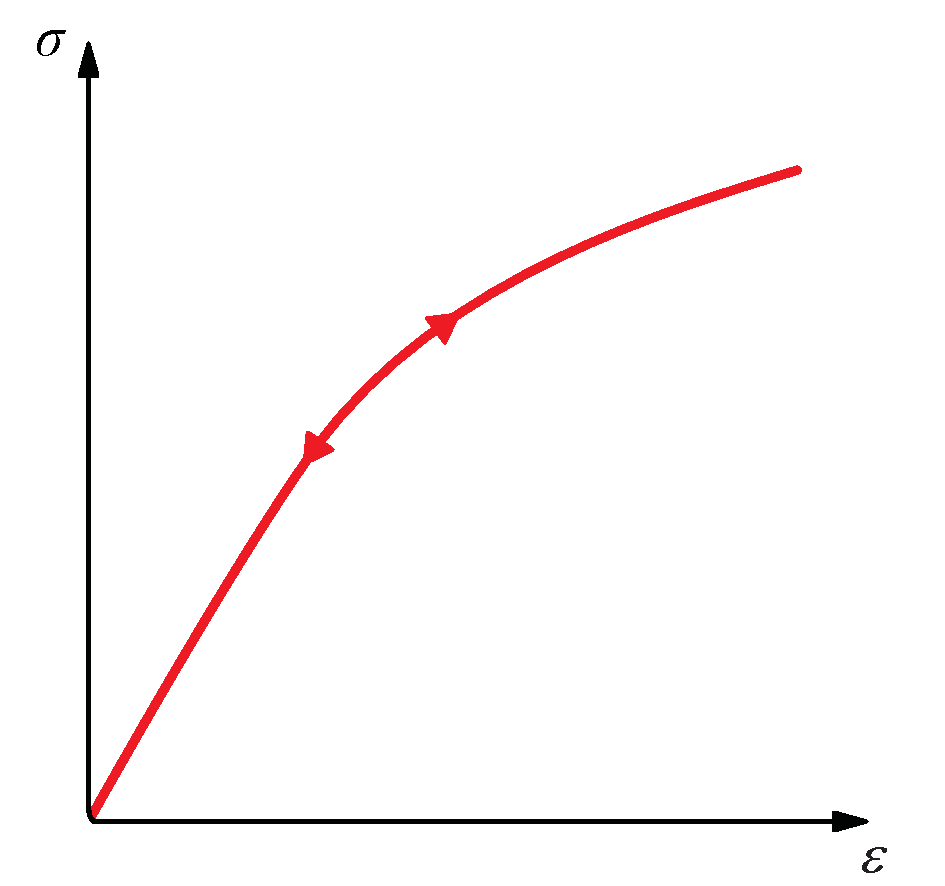
\includegraphics[width=0.4\textwidth,keepaspectratio=true]{figures/stress_strain_neo.pdf}
    \caption{Neo-hookean Stress-strain curve.}
    \label{fig:smm:cl:neo_hookean}
  \end{center}
\end{figure}

As illustrated in Figure~\ref{fig:smm:cl:neo_hookean}, the behavior is initially
linear and the mechanical behavior is very close to the corresponding linear
elastic material. This constitutive relationship, which accounts for compressibility,
 is a modified version of the one proposed by Ronald Rivlin \cite{Belytschko:2000}.

The strain energy stored in the material is given by:
\begin{equation}\label{eqn:smm:constitutive:neohookean_potential}
  \Psi(\mat{C}) = \frac{1}{2}\lambda_0\left(\ln J\right)^2-\mu_0\ln J+\frac{1}{2}
\mu_0\left(\text{trace}(\mat{C})-3\right)
\end{equation}
\noindent where $\lambda_0$ and $\mu_0$ are, respectively, Lamé's first parameter
and the shear modulus at the initial configuration. $J$ is the jacobian of the deformation
gradient ($\mat{F}=\nabla_{\!\!\vec{X}}\vec{x}$): $J=\text{det}(\mat{F})$. Finally $\mat{C}$ is the right Cauchy-Green
deformation tensor.

Since this kind of material is used for large deformation problems, a
finite deformation framework should be used. Therefore, the Cauchy
stress ($\mat{\sigma}$) should be computed through the second
Piola-Kirchhoff stress tensor $\mat{S}$:

\begin{equation}
  \mat{\sigma } = \frac{1}{J}\mat{F}\mat{S}\mat{F}^T
\end{equation}

Finally the second Piola-Kirchhoff stress tensor is given by:

\begin{equation}
  \mat{S}  = 2\frac{\partial\Psi}{\partial\mat{C}} = \lambda_0\ln J
\mat{C}^{-1}+\mu_0\left(\mat{I}-\mat{C}^{-1}\right)
\end{equation}

The parameters to indicate in the material file are the same
as those for the elastic case: \code{E} (Young's modulus), \code{nu} (Poisson's
ratio).

\subsection{Small-Deformation Plasticity}\index{Material!Small-deformation Plasticity}


The small-deformation plasticity is a simple plasticity material
formulation which accounts for the additive decomposition of strain
into elastic and plastic strain components. This formulation is
applicable to infinitesimal deformation where the additive
decomposition of the strain is a valid approximation. In this
formulation, plastic strain is a shearing process where hydrostatic
stress has no contribution to plasticity and consequently plasticity
does not lead to volume change. Figure ~\ref{fig:Lin-strain-hard}
shows the linear strain hardening elasto-plastic behavior according to
the additive decomposition of strain into the elastic and plastic
parts in infinitesimal deformation as


\begin{equation} \label{eqn:smm:constitutive:strain decomposition}
	\mat{\varepsilon} = \mat{\varepsilon}^e +\mat{\varepsilon}^p
\end{equation}  
\begin{equation} \label{eqn:smm:constitutive:Hooks law}
	{\mat{\sigma}} = 2G(\mat{\varepsilon}^e) + \lambda  trace(\mat{\varepsilon}^e)\mat{I}
\end{equation}

\noindent 
\begin{figure}[htp]
  \centering
   {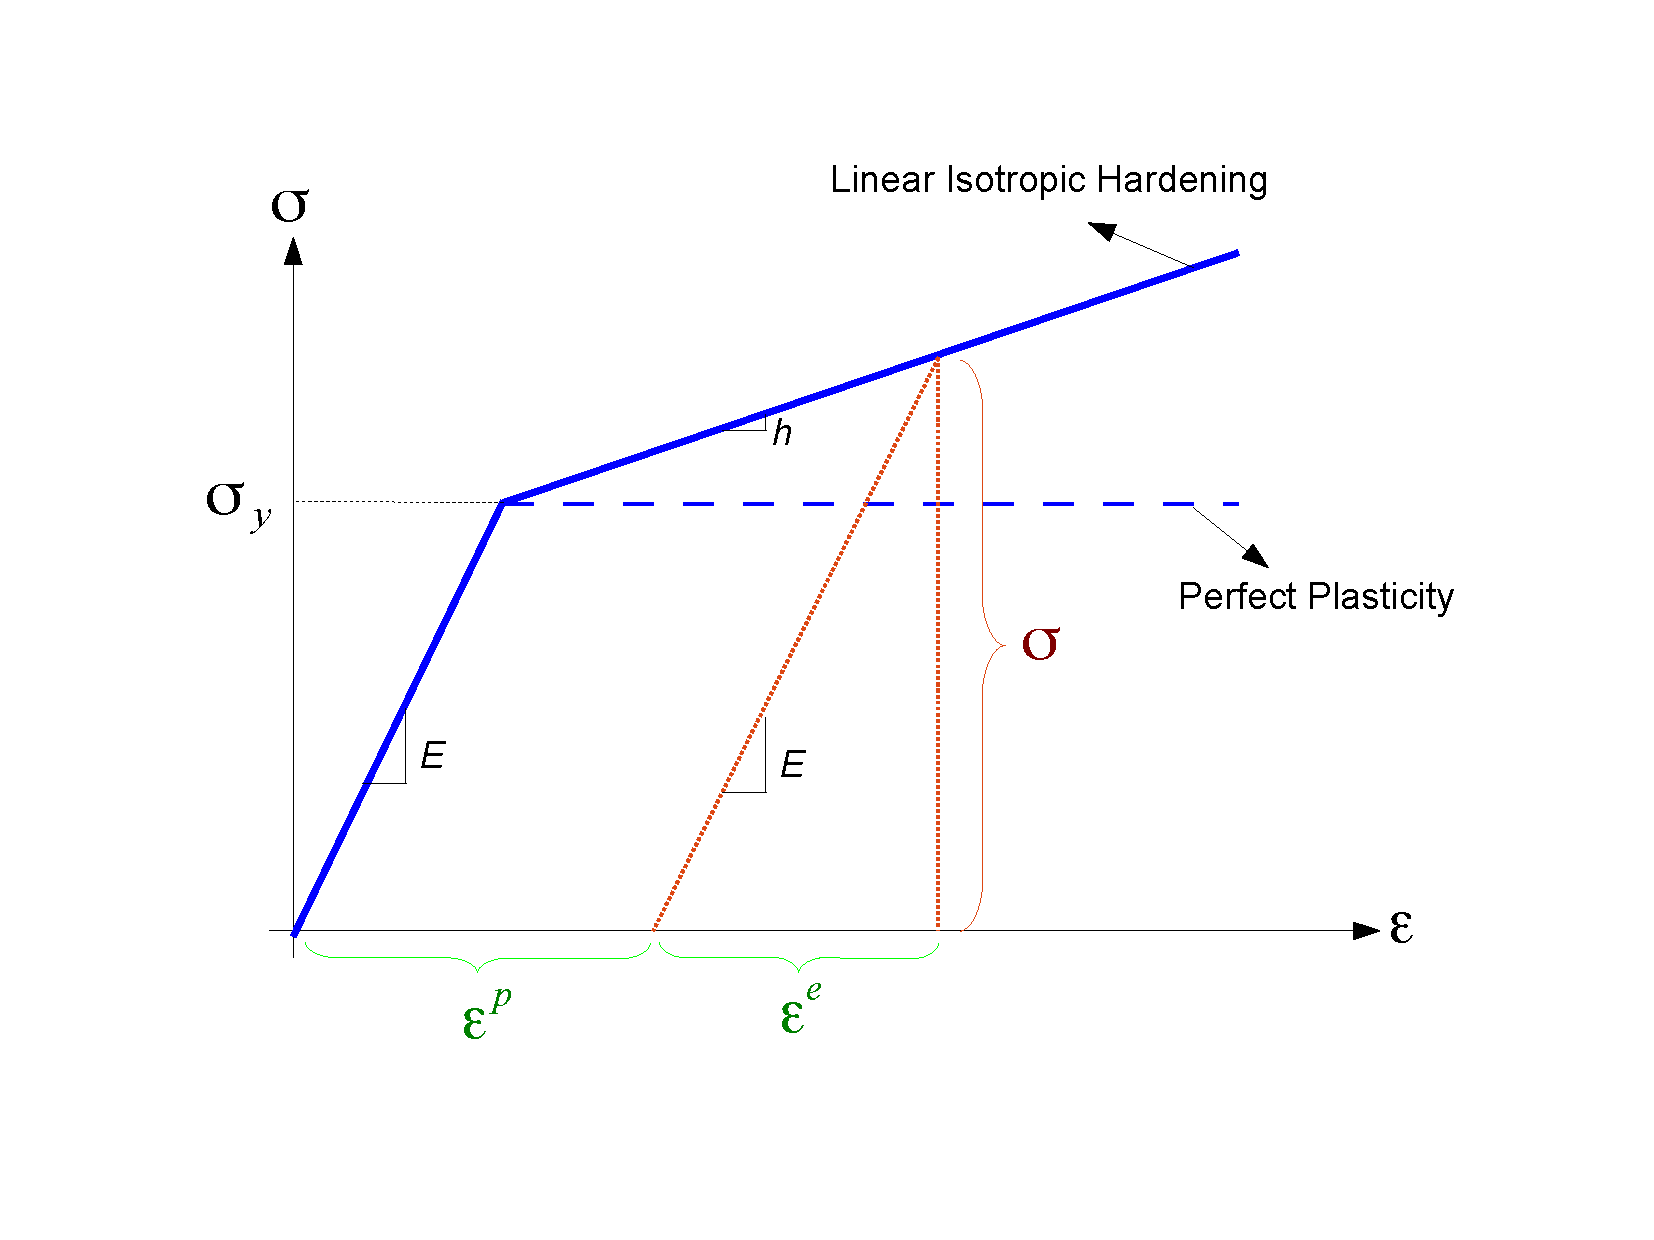
\includegraphics[scale=0.4, clip]{figures/isotropic_hardening_plasticity.pdf}}
   \caption{
    Stress-strain curve for the small-deformation plasticity with linear isotropic hardening.
   }
  \label{fig:smm:cl:Lin-strain-hard}
\end{figure}

\noindent In this class, the von Mises yield criterion is used. In the von Mises yield criterion, the yield is independent of the hydrostatic stress. Other yielding criteria such as Tresca and Gurson can be easily implemented in this class as well.

In the von Mises yield criterion, the hydrostatic stresses have no effect on the plasticity and consequently the yielding occurs when a critical elastic shear energy is achieved.

\begin{equation} \label{eqn:smm:constitutive:von Mises}
	f = \sigma_{\st{eff}} - \sigma_y = (\frac{3}{2} {\mat{\sigma}}^{\st{tr}} : {\mat{\sigma}}^{\st{tr}})^{1/2}-\sigma_y (\mat{\varepsilon}^p)
\end{equation}

\begin{equation} \label{eqn:smm:constitutive:yielding}
 	f < 0 \quad \textrm{Elastic deformation,} \qquad f = 0 \quad  \textrm{Plastic deformation}
\end{equation}

where $\sigma_y$ is the yield strength of the material which can be function of plastic strain in case of hardening type of materials and ${\mat{\sigma}}^{\st{tr}}$ is the deviatoric part of stress given by

\begin{equation} \label{eqn:smm:constitutive:deviatoric stress}
	{\mat{\sigma}}^{\st{tr}}=\mat{\sigma} - \frac{1}{3} trace(\mat{\sigma}) \mat {I}
\end{equation} 

After yielding $(f = 0)$, the normality hypothesis of plasticity determines the direction of plastic flow which is normal to the tangent to the yielding surface at the load point. Then, the tensorial form of the plastic constitutive equation using the von Mises yielding criterion (see equation 4.34) may be written as

\begin{equation} \label{eqn:smm:constitutive:plastic contitutive equation}
	\Delta {\mat{\varepsilon}}^p = \Delta p \frac {\partial{f}}{\partial{\mat \sigma}}=\frac{3}{2} \Delta p \frac{{\mat{\sigma}}^{\st{tr}}}{\sigma_{\st{eff}}}
\end{equation}

In these expressions, the direction of the plastic strain increment (or equivalently, plastic strain rate) is given by $\frac{{\mat{\sigma}}^{\st{tr}}}{\sigma_{\st{eff}}}$ while the magnitude is defined by the plastic multiplier $\Delta p$. This can be obtained using the \emph{consistency condition} which impose the requirement for the load point to remain on the yielding surface in the plastic regime.

\begin{table}[h]
\centering
  \begin{tabular}{| c | l | c |}
    \hline
    1 & Compute the trial stress & ${\mat{\sigma}}^{\st{tr}} = {\mat{\sigma}}_t + 2G\Delta \mat{\varepsilon} + \lambda trace(\Delta \mat{\varepsilon})\mat{I}$ \\[2ex] \hline
    2 & Check the Yielding criteria & $f = (\frac{3}{2} {\mat{\sigma}}^{\st{tr}} : {\mat{\sigma}}^{\st{tr}})^{1/2}-\sigma_y (\mat{\varepsilon}^p)$ \\[2ex] \hline
    3 & Compute the Plastic multiplier & \begin{tabular}{@{}c@{}c@{}} $d \Delta p = \frac{\sigma^{tr}_{eff} - 3G \Delta P^{(k)}- \sigma_y^{(k)}}{3G + h}		
$ \\ $\Delta p^{(k+1)}=\Delta p^{(k)}+ d\Delta p$ \\$\sigma_y^{(k+1)}=(\sigma_y)_t+ h\Delta p$ \end{tabular}\\ [2ex] \hline
    4 & Compute the plastic strain increment & $\Delta {\mat{\varepsilon}}^p = \frac{3}{2} \Delta p \frac{{\mat{\sigma}}^{\st{tr}}}{\sigma_{\st{eff}}}$ \\[2ex] \hline
    5 & Compute the stress increment & ${\Delta \mat{\sigma}} = 2G(\Delta \mat{\varepsilon}-\Delta \mat{\varepsilon}^p) + \lambda  trace(\Delta \mat{\varepsilon}-\Delta \mat{\varepsilon}^p)\mat{I}$ \\[2ex] \hline
    6 & Update the variables & \begin{tabular}{@{}c@{}} ${\mat{\varepsilon^p}}={\mat{\varepsilon}}^p_t+{\Delta {\mat{\varepsilon}}^p}$ \\    ${\mat{\sigma}}={\mat{\sigma}}_t+{\Delta \mat{\sigma}}$ \end{tabular}\\ [2ex] \hline     
    
  \end{tabular}
  \caption{Summary of the implementation procedure of small-deformation plasticity with linear isotropic hardening in \akantu}
  \label{table:equation for small-def plasticity with lin-iso-hardening}
\end{table}


Here, we summarize the implementation procedures for the
small-deformation plasticity with linear isotropic hardening. We use
an implicit integration technique called \emph{the radial return
  method} to obtain the plastic multiplier. This method has the
advantage of being unconditionally stable, however, the accuracy
remains dependent on the step size. The plastic parameters to indicate
in the material file are: \code{$\sigma_y$} (Yield stress) and
\code{h} (Hardening modulus). In addition, the elastic parameters need
to be defined as previously mentioned: \code{E} (Young's modulus),
\code{nu} (Poisson's ratio).


\subsection{Visco-Elasticity}

% Standard Solid rheological model, see [] J.C. Simo, T.J.R. Hughes,
% "Computational Inelasticity", Springer (1998), see Sections 10.2 and 10.3
Visco-elasticity is characterized by strain rate dependent
behavior. Moreover, when such a material undergoes a deformation it
dissipates energy. This dissipation results in a hysteresis loop in
the stress-strain curve at every loading cycle (see
Figure~\ref{fig:smm:cl:visco-elastic:hyst}). In principle, it can be
applied to many materials, since all materials exhibit a visco-elastic
behavior if subjected to particular conditions (such as high
temperatures).
\begin{figure}[!htb]
  \begin{center}

    \subfloat[]{
      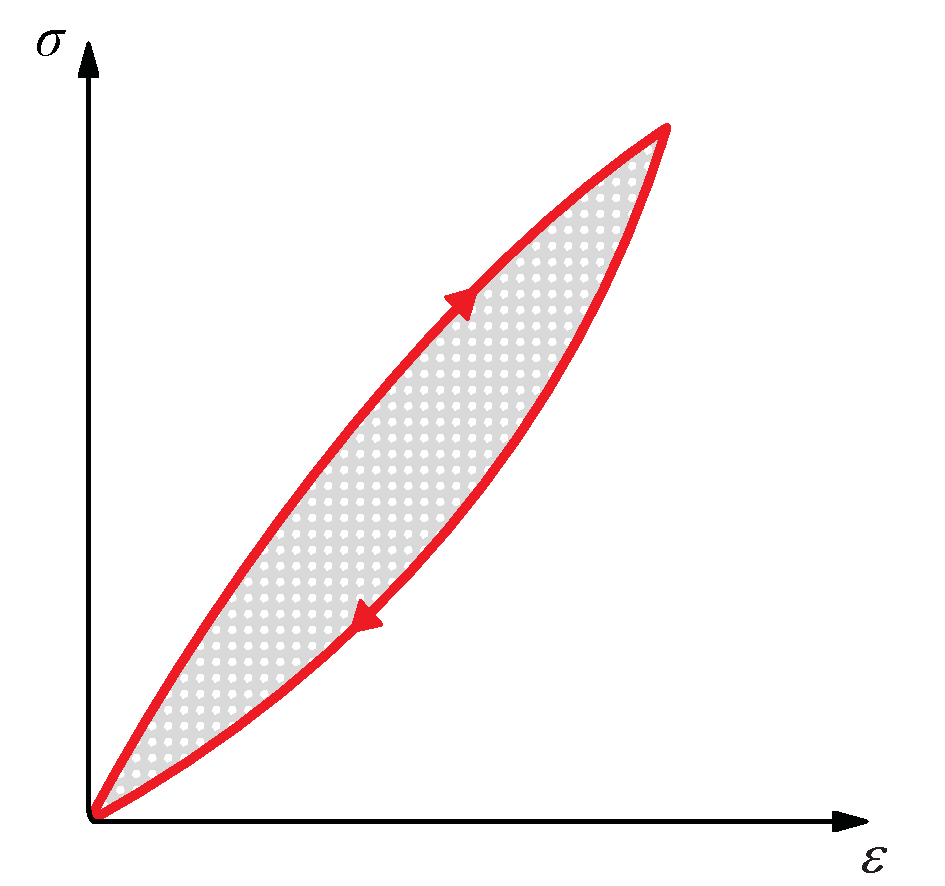
\includegraphics[width=0.4\textwidth,keepaspectratio=true]{figures/stress_strain_visco.pdf}
      \label{fig:smm:cl:visco-elastic:hyst}
    }
    \hspace{0.05\textwidth}
    \subfloat[]{
      \raisebox{0.025\textwidth}{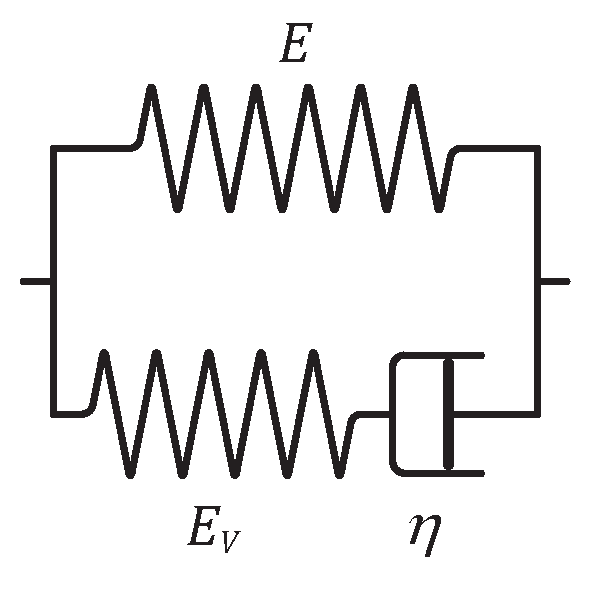
\includegraphics[width=0.3\textwidth,keepaspectratio=true]{figures/visco_elastic_law.pdf}}
      \label{fig:smm:cl:visco-elastic:model}
    }
    \caption{(a) Characteristic stress-strain behavior of a visco-elastic material with hysteresis loop and (b) schematic representation of the standard rheological linear solid visco-elastic model.}
    \label{fig:smm:cl:visco-elastic}
  \end{center}
\end{figure}
The standard rheological linear solid model (see Sections 10.2 and 10.3
of~\cite{simo92}) has been implemented in \akantu. This model results from the
combination of a spring mounted in parallel with a spring and a dashpot
connected in series, as illustrated in
Figure~\ref{fig:smm:cl:visco-elastic:model}. The advantage of this model is that
it allows to account for creep or stress relaxation. The equation that relates
the stress to the strain is (in 1D):
\begin{equation}
  \frac{d\epsilon(t)}{dt} = \left ( E + E_V \right ) ^ {-1} \cdot \left [ \frac{d\sigma(t)}{dt} + \frac{E_V}{\eta}\sigma(t) - \frac{EE_V}{\eta}\epsilon(t) \right ]
\end{equation}
where $\eta$ is the viscosity. The equilibrium condition is unique and
is attained in the limit, as $t \to \infty $. At this stage, the
response is elastic and depends on the Young's modulus $E$.  The
mandatory parameters for the material file are the following:
\code{rho} (density), \code{E} (Young's modulus), \code{nu} (Poisson's
ratio), \code{Plane\_Stress} (if set to zero plane strain, otherwise
plane stress), \code{eta} (dashpot viscosity) and \code{Ev} (stiffness
of the viscous element).

Note that the current standard linear solid model is applied only on the deviatoric part of the strain tensor. The spheric part of the strain tensor affects the stress tensor like an linear elastic material.

\subsection{Damage}

In the  simplified case of a  linear elastic and brittle  material, isotropic
damage can be represented by a scalar variable $d$, which varies from $0$ to $1$
for  no  damage  to  fully  broken  material  respectively.  The  stress-strain
relationship then becomes:
\begin{equation*}
  \mat{\sigma} = (1-d)\, \mat{C}:\mat{\varepsilon}
\end{equation*}

where  $\mat{\sigma}$,  $\mat{\varepsilon}$ are  the  Cauchy  stress and  strain
tensors, and $\mat{C}$ is the elastic stiffness tensor. This formulation relies
on the definition of an evolution law for the damage variable. In \akantu, many
possibilities exist and they are listed below.

\subsubsection{Marigo}
This damage evolution law is energy based as defined by Marigo \cite{marigo81a,
  lemaitre96a}. It is an isotropic damage law.
\begin{align}
  Y &= \frac{1}{2}\mat{\varepsilon}:\mat{C}:\mat{\varepsilon}\\
  F &= Y - Y_d - S d\\
  d &= \left\{
    \begin{array}{l l}
      \mathrm{min}\left(\frac{Y-Y_d}{S},\;1\right) & \mathrm{if}\; F > 0\\
      \mathrm{unchanged} & \mathrm{otherwise}
    \end{array}
  \right.
\end{align}
In this formulation, $Y$ is the strain energy release rate, $Y_d$ the
rupture criterion and $S$ the damage energy.  The non-local version of
this damage evolution law is constructed by averaging the energy $Y$.

\subsubsection{Mazars}
This law introduced by Mazars \cite{mazars84a} is a behavioral model to
represent damage evolution in concrete. The governing variable in this damage
law is the equivalent strain $\varepsilon_{\st{eq}} =
\sqrt{<\mat{\varepsilon}>_+:<\mat{\varepsilon}>_+}$, with $<.>_+$ the positive
part of the tensor.
The damage the is defined as:
\begin{align}
  D &= \alpha_t^\beta D_t + (1-\alpha_t)^\beta D_c\\
  D_t &= 1 - \frac{\kappa_0 (1- A_t)}{\varepsilon_{\st{eq}}} - A_t \exp^{-B_t(\varepsilon_{\st{eq}}-\kappa_0)}\\
  D_c &= 1 - \frac{\kappa_0 (1- A_c)}{\varepsilon_{\st{eq}}} - A_c
  \exp^{-B_c(\varepsilon_{\st{eq}}-\kappa_0)}\\
  \alpha_t &= \frac{\sum_{i=1}^3<\varepsilon_i>_+\varepsilon_{\st{nd}\;i}}{\varepsilon_{\st{eq}}^2}
\end{align}
With $\kappa_0$ the damage threshold, $A_t$ and $B_t$ the damage parameter in
traction, $A_c$ and $B_c$ the damage parameter in compression, $\beta$ is the
shear parameter. $\alpha_t$ is the coupling parameter between traction and
compression, the $\varepsilon_i$ are the eigenstrain and the
$\varepsilon_{\st{nd}\;i}$ are the eigenvalues of the strain if the material
were undamaged.

The coefficients $A$ and $B$ are the post-peak asymptotic
value and the decay shape parameters.


\subsection{Summary}\index{Material!List}

The list of all the materials available in Akantu is summarized in Tables \ref{tab:smm:cl:summary:list} as well as the keyword required for each material and the assosiated material properties.

\begin{table}[h!]
  \begin{center}
\begin{tabular}[c]{ m{3.5cm} | l | c | p{3.5cm} }
Material & Keyword & Parameter & Description \\
\hline
%%%%%%%%%%%%%%%%%
Linear elastic isotropic & \code{elastic} & -  & Table \ref{tab:smm:cl:summary:base}\\
\hline
%%%%%%%%%%%%%%%%%%
Linear elastic orthotropic  & \code{elastic\_orthotropic} & \code{Cij} & Tangent matrix coefficients (i,j = 1,2, ... voigt size ) \\
\hline
%%%%%%%%%%%%%%%%%%
Linear elastic anisotropic  & \code{elastic\_anisotropic} & \code{n1} & Direction of main material axis \\
 & & \code{n2} & Direction of secondary material axis \\
 & & \code{n3} & Direction of tertiery material axis \\
 & & \code{Cij} & Tangent matrix coefficients (i,j = 1,2, ... voigt size ) \\
 & & \code{alpha} & Proportion of viscous stress\\
\hline
%%%%%%%%%%%%%%%%%%
Neohookean (Finite-strain) \cite{Belytschko:2000} & \code{neohookean} & -  & Table \ref{tab:smm:cl:summary:base}\\
\hline
%%%%%%%%%%%%%%%%%%
Standard linear solid \cite{simo92} & \multirow{2}{*}{\code{sls\_deviatoric}} & - & Table \ref{tab:smm:cl:summary:base}\\
 & &  \code{Eta} & Viscosity\\
 & & \code{Ev} & Stiffness of the viscous element \\
\hline
%%%%%%%%%%%%%%%%%%
Elasto-plastic linear isotropic hardening & \code{plastic\_linear\_isotropic\_hardening}  & - & Table \ref{tab:smm:cl:summary:base}\\
 & &  \code{h} & Hardening modulus\\
 & &  \code{sigma\_y} & Yielding stress\\
\hline
%%%%%%%%%%%%%%%%%%
Visco-plastic & \code{visco\_plastic}  & - & Table \ref{tab:smm:cl:summary:base}\\
 & &  \code{rate} & Rate sensitivity component\\
 & &  \code{edot0} & Reference strain rate\\
 & &  \code{ts} & Time \\
\hline
\end{tabular}
\end{center}
  \caption{List of material properties with their corresponding keywords and material parameters.}
  \label{tab:smm:cl:summary:list}
\end{table}

\vspace{0.5cm}

In addition to the properties presented in Table \ref{tab:smm:cl:summary:list}, every material also has the parameter ''\code{rho}`` which corresponds to the density. The properties listed in Table  \ref{tab:smm:cl:summary:base} correspond to the parameters required to describe a linear elastic isotropic material, however those parameters are also commun to most of the materials available as previously described in Table \ref{tab:smm:cl:summary:list}.

\begin{table}[h!]
  \begin{center}
\begin{tabular}[c]{  l | p{6.5cm} }\label{tab:smm:cl:summary:base}
Parameter & Description \\
\hline
%%%%%%%%%%%%%%%%%
\code{rho}  & Density\\
\code{E}  & Young's modulus\\
\code{nu}  & Poisson's ratio\\
\code{Plane\_Stress} & Plane stress simplification (only 2D problems)\\
\hline
\end{tabular}
\end{center}
  \caption{List of material parameters shared my most materials}
  \label{tab:smm:cl:summary:base}
\end{table}

%%% Local Variables:
%%% mode: latex
%%% TeX-master: "manual"
%%% End:
}{}

\IfFileExists{manual-cohesive_laws.tex}{\subsection{Cohesive laws}
\label{sec:cohesive-laws}

\subsubsection{Linear Irreversible Law\matlabel{ssect:smm:cl:coh-snozzi}}

\begin{figure}[!hbt]
  \centering
  \subfloat[Linear]{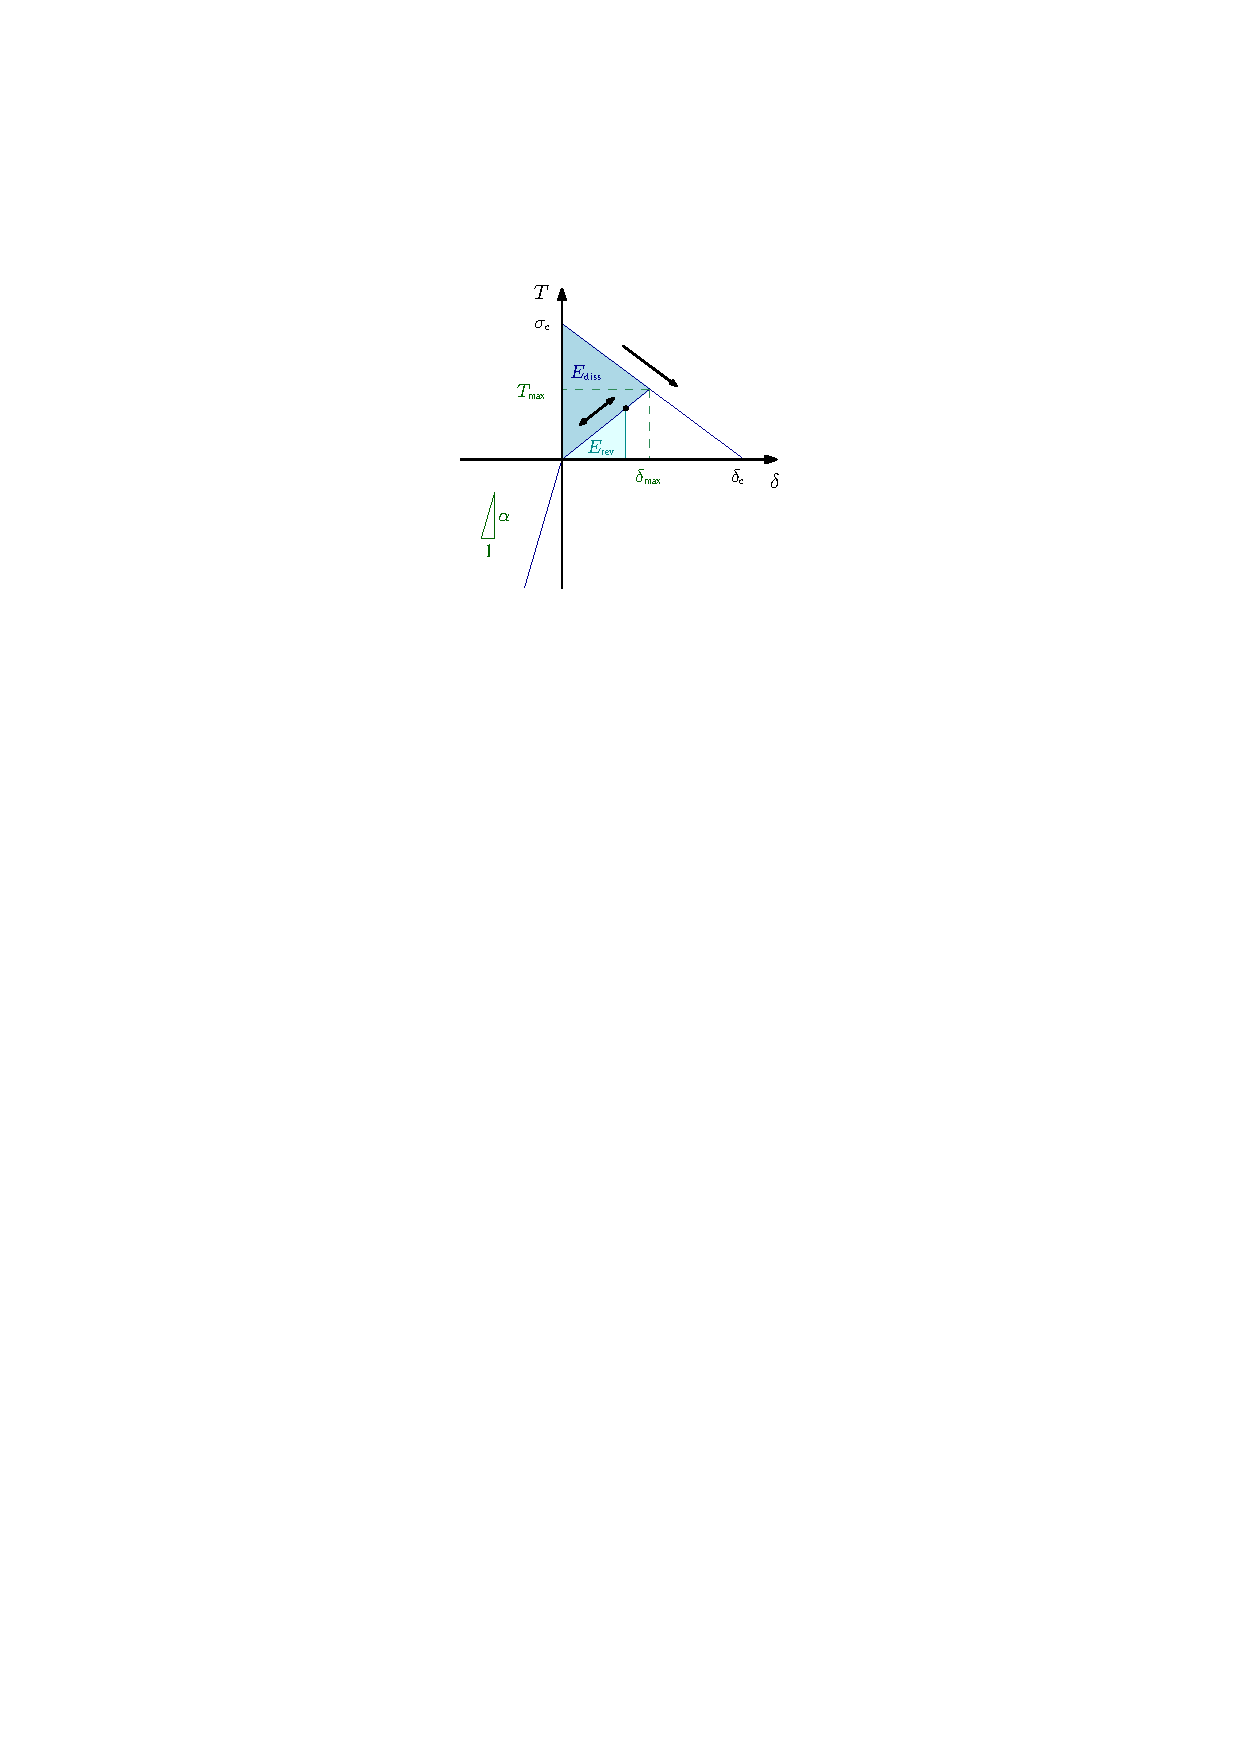
\includegraphics[width=0.4\textwidth]{figures/linear_cohesive_law}}
  \qquad
  \subfloat[Bilinear]{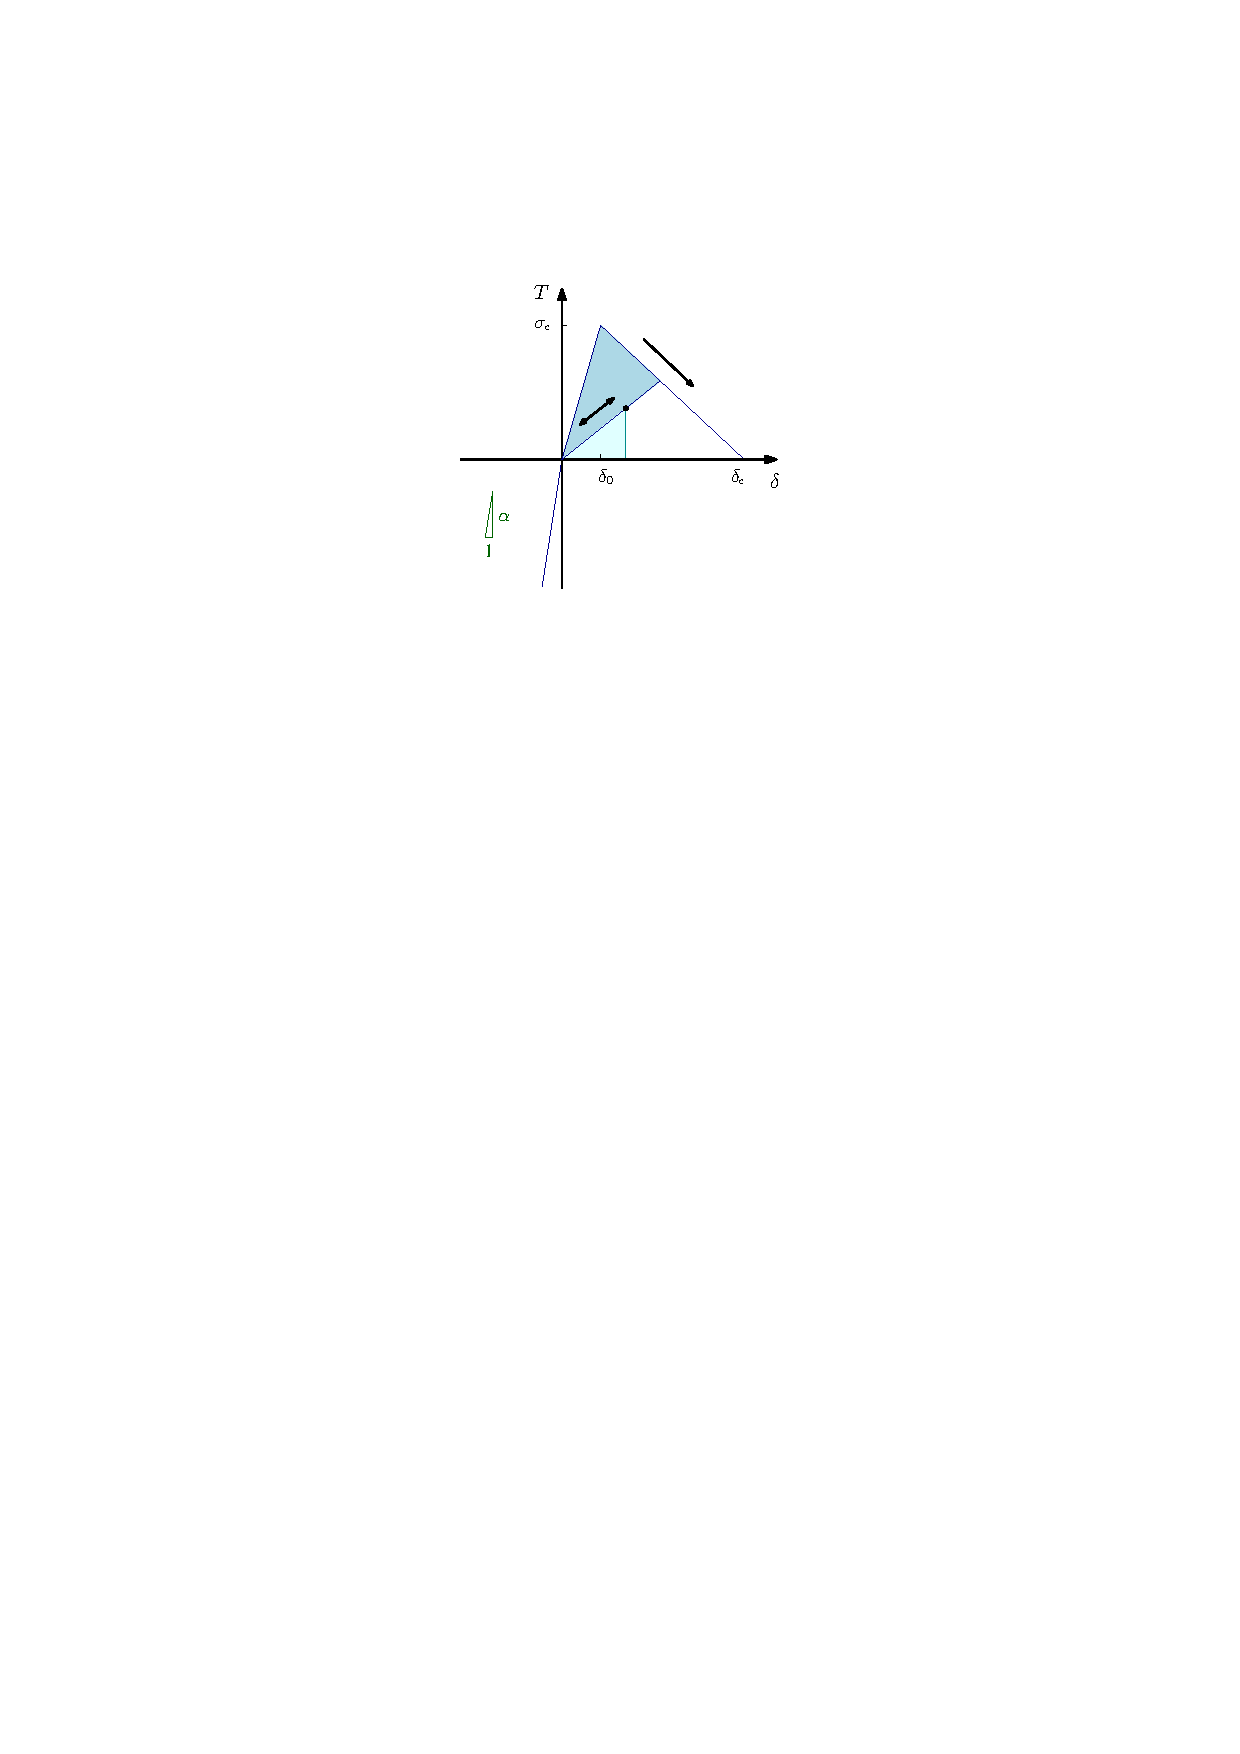
\includegraphics[width=0.4\textwidth]{figures/bilinear_cohesive_law}}
  \caption{Irreversible cohesive laws for explicit simulations.}
  \label{fig:smm:coh:linear_cohesive_law}
\end{figure}

\akantu includes the Snozzi-Molinari~\cite{snozzi_cohesive_2013}
linear irreversible cohesive law (see
Figure~\ref{fig:smm:coh:linear_cohesive_law}). It is an extension to
the Camacho-Ortiz~\cite{camacho_computational_1996} cohesive law in
order to make dissipated fracture energy path-dependent. The concept
of free potential energy is dropped and a new independent parameter
$\kappa$ is introduced:
\begin{equation}
  \kappa = \frac{G_\mathrm{c, II}}{G_\mathrm{c, I}}
\end{equation}

where $G_\mathrm{c, I}$ and $G_\mathrm{c, II}$ are the
necessary works of separation per unit area to open completely a
cohesive zone under mode I and mode II, respectively. Their model yields to the
following equation for cohesive tractions $\vec{T}$ in case of crack
opening ${\delta}$:
\begin{equation}
  \label{eq:smm:coh:tractions}
  \vec{T} = \left( \frac{\beta^2}{\kappa} \Delta_\mathrm{t} \vec{t} +
    \Delta_\mathrm{n} \vec{n} \right)
  \frac{\sigma_\mathrm{c}}{\delta}
  \left( 1- \frac{\delta}{\delta_\mathrm{c}} \right)
  = \hat{\vec T}\,
  \frac{\sigma_\mathrm{c}}{\delta}
  \left( 1- \frac{\delta}{\delta_\mathrm{c}} \right)
\end{equation}

where $\sigma_\mathrm{c}$ is the material strength along the fracture,
$\delta_\mathrm{c}$ the critical effective displacement after which
cohesive tractions are zero (complete decohesion), $\Delta_\mathrm{t}$
and $\Delta_\mathrm{n}$ are the tangential and normal components of
the opening displacement vector $\vec{\Delta}$, respectively. The
parameter $\beta$ is a weight that indicates how big the tangential
opening contribution is. The effective opening displacement is:
\begin{equation}
  \delta = \sqrt{\frac{\beta^2}{\kappa^2} \Delta_\mathrm{t}^2 +
    \Delta_\mathrm{n}^2}
\end{equation}
In case of unloading or reloading $\delta < \delta_\mathrm{max}$,
tractions are calculated as:
\begin{align}
  T_\mathrm{n} &= \Delta_\mathrm{n}\,
  \frac{\sigma_\mathrm{c}}{\delta_\mathrm{max}}
  \left( 1- \frac{\delta_\mathrm{max}}{\delta_\mathrm{c}} \right) \\
  T_\mathrm{t} &= \frac{\beta^2}{\kappa}\, \Delta_\mathrm{t}\,
  \frac{\sigma_\mathrm{c}}{\delta_\mathrm{max}}
  \left( 1- \frac{\delta_\mathrm{max}}{\delta_\mathrm{c}} \right)
\end{align}
so that they vary linearly between the origin and the maximum attained
tractions. As shown in Figure~\ref{fig:smm:coh:linear_cohesive_law},
in this law, the dissipated and reversible energies are:
\begin{align}
  E_\mathrm{diss} &= \frac{1}{2} \sigma_\mathrm{c}\, \delta_\mathrm{max}\\[1ex]
  E_\mathrm{rev} &= \frac{1}{2} T\, \delta
\end{align}
Moreover, a damage parameter $D$ can be defined as:
\begin{equation}
  D = \min \left(
    \frac{\delta_\mathrm{max}}{\delta_\mathrm{c}},1 \right)
\end{equation}
which varies from 0 (undamaged condition) and 1 (fully
damaged condition). This variable can only increase because damage is
an irreversible process. A simple penalty contact model has been incorporated
in the cohesive law so that normal tractions can be returned in
case of compression:
\begin{equation}
  T_\mathrm{n} = \alpha \Delta_\mathrm{n} \quad\text{if
    $\Delta_\mathrm{n} < 0$}
\end{equation}
where $\alpha$ is a stiffness parameter that defaults to zero. The
relative contact energy is equivalent to reversible energy but in
compression.

The material name of the linear decreasing cohesive law  is
\code{material\_cohesive\_linear} and its parameters with their
respective default values are:
\begin{itemize}
\item \code{sigma\_c}: 0
\item \code{delta\_c}: 0
\item \code{beta}: 0
\item \code{G\_c}: 0
\item \code{kappa}: 1
\item \code{penalty}: 0
\end{itemize}
where \code{G\_c} corresponds to $G_\mathrm{c, I}$. A random number
generator can be used to assign a random $\sigma_\mathrm{c}$ to each
facet following a given distribution (see
Section~\ref{sect:smm:CL}). Only one parameter between \code{delta\_c}
and \code{G\_c} has to be specified. For random $\sigma_\mathrm{c}$
distributions, the chosen parameter of these two is kept fixed and the
other one is varied.

The bilinear constitutive law works exactly the same way as the linear
one, except for the additional parameter \code{delta\_0} that by
default is zero. Two examples for the extrinsic and intrinsic cohesive
elements and also an example to assign different properties to
intergranular and transgranular cohesive elements can be found in
the folder \code{\examplesdir/cohesive\_element/}.

\subsubsection{Linear Cohesive Law with Fatigue\matlabel{ssect:smm:cl:coh-fatigue}}

This law represents a variation of the linear irreversible cohesive
law of the previous section, that removes the hypothesis of elastic
unloading-reloading cycles. With this law, some energy is dissipated
also during unloading and reloading with hysteresis. The
implementation follows the work of~\cite{nguyen2001}. During the
unloading-reloading cycle, the traction increment is computed as
\begin{equation}
  \dot{T} =
  \begin{cases}
    K^- \, \dot{\delta} & \text{if $\dot{\delta} < 0$} \\
    K^+ \, \dot{\delta} & \text{if $\dot{\delta} > 0$} \\
  \end{cases}
\end{equation}
where $\dot{\delta}$ and $\dot{T}$ are respectively the effective
opening displacement and the cohesive traction increments with respect
to time, while $K^-$ and $K^+$ are respectively the unloading and
reloading incremental stiffness. The unloading path is linear and
results in an unloading stiffness
\begin{equation}
  K^- = \frac{T_\mathrm{max}}{\delta_\mathrm{max}}
\end{equation}
where $T_\mathrm{max}$ and $\delta_\mathrm{max}$ are the maximum
cohesive traction and the effective opening displacement reached
during the precedent loading phase. The unloading stiffness remains
constant during the unloading phase. On the other hand the reloading
stiffness increment $\dot{K}^+$ is calculated as
\begin{equation}
  \dot{K}^+ =
  \begin{cases}
    - K^+ \, \dot{\delta} / \delta_\mathrm{f} & \text{if $\dot{\delta}
      > 0$} \\
    \left( K^+ - K^- \right) \, \dot{\delta} / \delta_\mathrm{f} &
    \text{if $\dot{\delta} < 0$}
  \end{cases}
\end{equation}
where $\delta_\mathrm{f}$ is a material parameter. During unloading
the stiffness $K^+$ tends to $K^-$, while during reloading $K^+$ gets
decreased at every time step. If the cohesive traction during
reloading exceeds the upper limit given by
equation~\eqref{eq:smm:coh:tractions}, it is recomputed following the
behavior of the linear decreasing cohesive law for crack opening.

\subsubsection{Exponential Cohesive Law\matlabel{ssect:smm:cl:coh-exponential}}

Ortiz and Pandolfi proposed this cohesive law in 1999~\cite{ortiz1999}.  The
traction-opening equation for this law is as follows:
\begin{equation}
  \label{eq:exponential_law}
  T = e \sigma_c \frac{\delta}{\delta_c}e^{-\delta/ \delta_c}
\end{equation}
This equation is plotted in Figure~\ref{fig:smm:CL:ECL}. The term
$\partial{\vec{T}}/ \partial{\delta}$ of
equation~\eqref{eq:cohesive_stiffness} after the necessary derivation
can expressed as
\begin{equation}
  \label{eq:tangent_cohesive}
  \frac{\partial{\vec{T}}} {\partial{\delta}} = \hat{\vec{T}} \otimes
  \frac                       {\partial{(T/\delta)}}{\partial{\delta}}
  \frac{\hat{\vec{T}}}{\delta}+ \frac{T}{\delta}  \left[ \beta^2 \mat{I} +
  \left(1-\beta^2\right) \left(\vec{n} \otimes \vec{n}\right)\right]
\end{equation}
where
\begin{equation}
  \frac{\partial{(T/ \delta)}}{\partial{\delta}} = \left\{\begin{array} {l l}
      -e  \frac{\sigma_c}{\delta_c^2  }e^{-\delta  /  \delta_c} &  \quad  if
      \delta \geq \delta_{max}\\
      0 & \quad if \delta < \delta_{max}, \delta_n > 0
    \end{array} \right.
\end{equation}


\begin{figure}[!htb]
  \begin{center}
    \includegraphics[width=0.6\textwidth,keepaspectratio=true]{figures/cohesive_exponential.pdf}
    \caption{Exponential cohesive law}
    \label{fig:smm:CL:ECL}
  \end{center}
\end{figure}


%%% Local Variables:
%%% mode: latex
%%% TeX-master: "manual"
%%% End:
}{}


%%% Local Variables:
%%% mode: latex
%%% TeX-master: "manual"
%%% End:


\section{Adding a New Constitutive Law}\index{Material!create a new
material}

There are several constitutive laws in \akantu as described in the
previous Section~\ref{sect:smm:CL}. It is also possible to use a
user-defined material for the simulation. These materials are referred
to as local materials since they are local to the example of the user
and not part of the \akantu library.  To define a new local material,
two files (\code {material\_XXX.hh} and \code{material\_XXX.cc}) have
to be provided where \code{XXX} is the name of the new material. The
header file \code {material\_XXX.hh} defines the interface of your
custom material. Its implementation is provided in the
\code{material\_XXX.cc}. The new law must inherit from the
\code{Material} class or any other existing material class. It is
therefore necessary to include the interface of the parent material
in the header file of your local material and indicate the inheritance
in the declaration of the class:
\begin{cpp}
/* ---------------------------------------------------------------------- */
#include "material.hh"
/* ---------------------------------------------------------------------- */

#ifndef __AKANTU_MATERIAL_XXX_HH__
#define __AKANTU_MATERIAL_XXX_HH__

__BEGIN_AKANTU__

class MaterialXXX : public Material {

/// declare here the interface of your material

};
\end{cpp}
In the header file the user also needs to declare all the members of the new
material. These include the parameters that a read from the
material input file, as well as any other material parameters that will be
computed during the simulation and internal variables.


In the following the example of adding a new damage material will be
presented. In this case the parameters in the material will consist of the
Young's modulus, the Poisson coefficient, the resistance to damage and the
damage threshold. The material will then from these values compute its Lam\'{e}
coefficients and its bulk modulus. Furthermore, the user has to add a new
internal variable \code{damage} in order to store the amount of damage at each
quadrature point in each step of the simulation. For this specific material the
member declaration inside the class will look as follows:
\begin{cpp}
class LocalMaterialDamage : public Material {

/// declare constructors/destructors here

/// declare methods and accessors here

  /* -------------------------------------------------------------------- */
  /* Class Members                                                        */
  /* -------------------------------------------------------------------- */

  AKANTU_GET_MACRO_BY_ELEMENT_TYPE_CONST(Damage, damage, Real);
private:

  /// the young modulus
  Real E;

  /// Poisson coefficient
  Real nu;

  /// First Lame coefficient
  Real lambda;

  /// Second Lame coefficient (shear modulus)
  Real mu;

  /// resistance to damage
  Real Yd;

  /// damage threshold
  Real Sd;

  /// Bulk modulus
  Real kpa;

  /// damage internal variable
  InternalField<Real> damage;

};
\end{cpp}
In order to enable to print the material parameters at any point in
the user's example file using the standard output stream by typing:
\begin{cpp}
for (UInt m = 0; m  < model.getNbMaterials(); ++m)
  std::cout << model.getMaterial(m) << std::endl;
\end{cpp}
the standard output stream operator has to be redefined. This should be done at the end of the header file:
\begin{cpp}
class LocalMaterialDamage : public Material {

  /// declare here the interace of your material

}:
/* ---------------------------------------------------------------------- */
/* inline functions                                                       */
/* ---------------------------------------------------------------------- */
/// standard output stream operator
inline std::ostream & operator <<(std::ostream & stream, const LocalMaterialDamage & _this)
{
  _this.printself(stream);
  return stream;
}
\end{cpp}
However, the user still needs to register the material parameters that
should be printed out. The registration is done during the call of the
constructor. Like all definitions the implementation of the
constructor has to be written in the \code{material\_XXX.cc}
file. However, the declaration has to be provided in the
\code{material\_XXX.hh} file:
\begin{cpp}
class LocalMaterialDamage : public Material {
  /* -------------------------------------------------------------------- */
  /* Constructors/Destructors                                             */
  /* -------------------------------------------------------------------- */
public:

  LocalMaterialDamage(SolidMechanicsModel & model, const ID & id = "");
};
\end{cpp}
The user can now define the implementation of the constructor in the
\code{material\_XXX.cc} file:
\begin{cpp}
/* ---------------------------------------------------------------------- */
#include "local_material_damage.hh"
#include "solid_mechanics_model.hh"

__BEGIN_AKANTU__

/* ---------------------------------------------------------------------- */
LocalMaterialDamage::LocalMaterialDamage(SolidMechanicsModel & model,
					 const ID & id)  :
  Material(model, id),
  damage("damage", *this) {
  AKANTU_DEBUG_IN();

  this->registerParam("E", E, 0., _pat_parsable, "Young's modulus");
  this->registerParam("nu", nu, 0.5, _pat_parsable, "Poisson's ratio");
  this->registerParam("lambda", lambda, _pat_readable, "First Lame coefficient");
  this->registerParam("mu", mu, _pat_readable, "Second Lame coefficient");
  this->registerParam("kapa", kpa, _pat_readable, "Bulk coefficient");
  this->registerParam("Yd", Yd,   50., _pat_parsmod);
  this->registerParam("Sd", Sd, 5000., _pat_parsmod);

  damage.initialize(1);

  AKANTU_DEBUG_OUT();
}
\end{cpp}
During the intializer list the reference to the model and the material id are
assigned and the constructor of the internal field is called. Inside the scope
of the constructor the internal values have to be initialized and the
parameters, that should be printed out, are registered with the function:
\code{registerParam}\index{Material!registerParam}:
\begin{cpp}
void registerParam(name of the parameter (key in the material file),
		   member variable,
		   default value (optional parameter),
		   access permissions,
		   description);
\end{cpp}
The available access permissions are as follows:
\begin{itemize}
  \item \code{\_pat\_internal}: Parameter can only be output when the material is printed.
  \item \code{\_pat\_writable}: User can write into the parameter. The parameter is output when the material is printed.
  \item \code{\_pat\_readable}: User can read the parameter. The parameter is output when the material is printed.
  \item \code{\_pat\_modifiable}: Parameter is writable and readable.
  \item \code{\_pat\_parsable}: Parameter can be parsed, \textit{i.e.} read from the input file.
  \item \code{\_pat\_parsmod}: Parameter is modifiable and parsable.
\end{itemize}

In order to implement the new constitutive law the user needs to
specify how the additional material parameters, that are not
defined in the input material file, should be calculated. Furthermore,
it has to be defined how stresses and the stable time step should be
computed for the new local material. In the case of implicit
simulations, in addition, the computation of the tangent stiffness needs
to be defined. Therefore, the user needs to redefine the following
functions of the parent material:
\begin{cpp}
void initMaterial();

// for explicit and implicit simulations void
computeStress(ElementType el_type, GhostType ghost_type = _not_ghost);

// for implicit simulations
void computeTangentStiffness(const ElementType & el_type,
			     Array<Real> & tangent_matrix,
			     GhostType ghost_type = _not_ghost);

// for explicit and implicit simulations
Real getStableTimeStep(Real h, const Element & element);
\end{cpp}
In the following a detailed description of these functions is provided:
\begin{itemize}

\item \code{initMaterial}:~ This method is called after the material
  file is fully read and the elements corresponding to each material
  are assigned. Some of the frequently used constant parameters are
  calculated in this method. For example, the Lam\'{e} constants of
  elastic materials can be considered as such parameters.

\item \code{computeStress}:~ In this method, the stresses are
  computed based on the constitutive law as a function of the  strains of the
  quadrature points.  For example, the stresses for the elastic
  material are calculated based on the following formula:
  \begin{equation}
    \label{eqn:smm:constitutive_elastic}
    \mat{\sigma }  =\lambda\mathrm{tr}(\mat{\varepsilon})\mat{I}+2 \mu \mat{\varepsilon}
  \end{equation}

  Therefore, this method contains a loop on all quadrature points
  assigned to the material using the two macros:\par
  \code{MATERIAL\_STRESS\_QUADRATURE\_POINT\_LOOP\_BEGIN}\par
  \code{MATERIAL\_STRESS\_QUADRATURE\_POINT\_LOOP\_END}

  \begin{cpp}
    MATERIAL_STRESS_QUADRATURE_POINT_LOOP_BEGIN(element_type);

    // sigma <- f(grad_u)

    MATERIAL_STRESS_QUADRATURE_POINT_LOOP_END;
  \end{cpp}

  \note{The strain vector in \akantu contains the values of $\nabla
\vec{u}$, i.e. it is really the \emph{displacement gradient},}

\item \code{computeTangentStiffness}:~ This method is called when
  the tangent to the stress-strain curve is desired (see Fig \ref
  {fig:smm:AL:K}).  For example, it is called in the implicit solver
  when the stiffness matrix for the regular elements is assembled
  based on the following formula:
  \begin{equation}
    \label{eqn:smm:constitutive_elasc} \mat{K }
    =\int{\mat{B^T}\mat{D(\varepsilon)}\mat{B}}
  \end{equation}

  Therefore, in this method, the \code{tangent} matrix (\mat{D}) is
  computed for a given strain.

  \note{ The \code{tangent} matrix is a $4^{th}$ order tensor which is
    stored as a matrix in Voigt notation.}

  \begin{figure}[!htb]
    \begin{center}
      \includegraphics[width=0.4\textwidth,keepaspectratio=true]{figures/tangent.pdf}
      \caption{Tangent to the stress-strain curve.}
      \label{fig:smm:AL:K}
    \end{center}
  \end{figure}

\item \code{getCelerity}:~The stability criterion of the explicit integration scheme depend on the fastest wave celerity~\eqref{eqn:smm:explicit:stabletime}. This celerity depend on the material, and therefore the value of this velocity should be defined in this method for each new material. By default, the fastest wave speed is the compressive wave whose celerity can be defined in~\code{getPushWaveSpeed}.
\end{itemize}
Once the declaration and implementation of the new material has been
completed, this material can be used in the user's example by including the header file:
\begin{cpp}
#include "material_XXX.hh"
\end{cpp}
For existing materials, as mentioned in Section~\ref{sect:smm:CL}, by
default, the materials are initialized inside the method
\code{initFull}. If a local material should be used instead, the
initialization of the material has to be postponed until the local
material is registered in the model. Therefore, the model is
initialized with the boolean for skipping the material initialization
equal to true:
\begin{cpp}
/// model initialization
model.initFull(SolidMechanicsModelOptions(_explicit_lumped_mass,true));
\end{cpp}
Once the model has been initialized, the local material needs
to be registered in the model:
\begin{cpp}
model.registerNewCustomMaterials<XXX>("name_of_local_material");
\end{cpp}
Only at this point the material can be initialized:
\begin{cpp}
model.initMaterials();
\end{cpp}
A full example for adding a new damage law can be found in
\shellcode{\examplesdir/new\_material}.

\subsection{Adding a New Non-Local Constitutive Law}\index{Material!create a new non-local material}

In order to add a new non-local material we first have to add the local constitutive law in \akantu (see above). We can then add the non-local version of the constitutive law by adding the two files (\code{material\_XXX\_non\_local.hh} and \code{material\_XXX\_non\_local.cc}) where \code{XXX} is the name of the corresponding local material. The new law must inherit from the two classes, non-local parent class, such as the \code{MaterialNonLocal} class, and from the local version of the constitutive law, \textit{i.e.} \code{MaterialXXX}. It is therefore necessary to include the interface of those classes in the header file of your custom material and indicate the inheritance in the declaration of the class:
\begin{cpp}
/* ---------------------------------------------------------------------- */
#include "material_non_local.hh" // the non-local parent
#include "material_XXX.hh"
/* ---------------------------------------------------------------------- */

#ifndef __AKANTU_MATERIAL_XXX_HH__
#define __AKANTU_MATERIAL_XXX_HH__

__BEGIN_AKANTU__

class MaterialXXXNonLocal : public MaterialXXX,
                            public MaterialNonLocal {

/// declare here the interface of your material

};
\end{cpp}
As members of the class we only need to add the internal fields to store the non-local quantities, which are obtained from the averaging process:
\begin{cpp}
/* -------------------------------------------------------------------------- */
/* Class members                                                              */
/* -------------------------------------------------------------------------- *
protected:
  InternalField<Real> grad_u_nl;
\end{cpp}
The following four functions need to be implemented in the non-local material:
\begin{cpp}
  /// initialization of the material
  void initMaterial();
  /// loop over all element and invoke stress computation
  virtual void computeNonLocalStresses(GhostType ghost_type);
  /// compute stresses after local quantities have been averaged
  virtual void computeNonLocalStress(ElementType el_type, GhostType ghost_type)
  /// compute all local quantities
  void computeStress(ElementType el_type, GhostType ghost_type);
\end{cpp}
In the intialization of the non-local material we need to register the local quantity for the averaging process. In our example the internal field \emph{grad\_u\_nl} is the non-local counterpart of the gradient of the displacement field (\emph{grad\_u\_nl}):
\begin{cpp}
  void MaterialXXXNonLocal::initMaterial() {
    MaterialXXX::initMaterial();
    MaterialNonLocal::initMaterial();
    /// register the non-local variable in the manager
    this->model->getNonLocalManager().registerNonLocalVariable(this->grad_u.getName(), this->grad_u_nl.getName(), spatial_dimension * spatial_dimension);

}
\end{cpp}
The function to register the non-local variable takes as parameters the name of the local internal field, the name of the non-local counterpart and the number of components of the field we want to average.
In the \emph{computeStress} we now need to compute all the quantities we want to average. We can then write a loop for the stress computation in the function \emph{computeNonLocalStresses} and then provide the constitutive law on each integration point in the function \emph{computeNonLocalStress}.



%%% Local Variables: %%% mode: latex %%% TeX-master: "manual" %%% End:


\IfFileExists{manual-structuralmechanicsmodel.tex}{\chapter{Structural  Mechanics   model}
Static    structural   mechanics    problems   can    be   handled    using   the
\code{StructuralMechanicsModel}.  So far, \akantu\  provides 2D and 3D Bernoulli
beam elements \cite{frey2009}.  Just  as for the \code{SolidMechanicsModel}, the
model  is created  for  a given  \code{Mesh}.   The model  will  create its  own
\code{FEM}  object  to  compute  the interpolation,  gradient,  integration  and
assembly  operations.  The  \code{StructuralMechanicsModel} constructor  is used
like

\begin{cpp}
  StructuralMechanicsModel model(mesh, spatial_dimension);
\end{cpp}
where \code{mesh} is  a \code{Mesh} object defining the  structure for which the
equations  of statics  are to  be solved,  and \code{spatial\_dimension}  is the
dimensionality  of the  problem.  If  \code{spatial\_dimension} is  omitted, the
problem is assumed  to have the same dimensionality as the  one specified by the
mesh.

\note[\ 1]{Dynamic computations are not supported to date.}

\note[\ 2]{Structural meshes are created and loaded as described in
  Section~\ref{sect:common:mesh} with \code{MeshIOMSHStruct} instead  of \code{MeshIOMSH}.}

\vspace{1cm}
This model contains at least the following \code{Arrays}:
\begin{description}
\item[boundary]  contains a  boolean  value for  each  degree of  freedom
  specifying  whether  that degree  is  blocked  or  not. A  Dirichlet  boundary
  condition can be prescribed by setting the \textbf{boundary} value of a degree
  of freedom to  \code{true}.  A Neumann boundary condition  can  be applied
  by setting the corresponding  \textbf{boundary} value to  \code{false}.
  The \textbf{displacement} is computed for all degrees of freedom for which the \textbf{boundary} value is set to \code{false}. For the remaining degrees of freedom, the imposed values (zero by default after initialization) are kept.
  

  
\item[displacement\_rotation]  contains  the  generalized displacements (displacements and rotations)  of  all
  degrees of freedom. It can be  either a computed displacement for free degrees
  of freedom  or an imposed displacement  in case of blocked  ones ($\vec{u}$ in
  the following).
  
\item[force\_moment]  contains the  generalized external  forces (forces and moments) applied  to the
  nodes ($\vec{f_{\st{ext}}}$ in the following).
  
\item[residual] contains the difference between external and internal forces and
  moments. On the blocked degrees of freedom, \textbf{residual} contains the support
  reactions   ($\vec{r}$ in  the following).   It should  be mentioned  that at
  equilibrium, \textbf{residual} should be zero on the free degrees of freedom.
\end{description}

An example to help understand how  to use this model will be presented in the
next section.

\section{Model setup}
\label{sec:structMechMod:setup}

\subsection{Initialization}
The easiest way to initialize the structural mechanics model is:
%\begin{cpp}
%  model.initModel();
%  
%  StructuralMaterial mat1;
%  mat1.E=2.05e11;
%  mat1.I=0.00128;
%  mat1.A=0.01; // for example
%
%  model.addMaterial(mat1); ASK NICO ABOUT THIS CRAP
%
%  model.initArrays();
%  model.initImplicitSolver();
%\end{cpp}
%The method \code{initModel} computes the shape functions, \code{addMaterial} sets the material parameters to be used, \code{initArrays} initializes all the internal arrays mentioned before and \code{initImplicitSolver} creates the stiffness matrix.

\begin{cpp}
  model.initFull();
\end{cpp}
The method \code{initFull} computes the shape functions, initializes the internal vectors mentioned above and allocates the memory for the stiffness matrix.

Material  properties are  defined using  the \code{StructuralMaterial}
structure described in Table~\ref{tab:structMechMod:strucMaterial}. Such a definition could for instance look like
\begin{cpp}
  StructuralMaterial mat;
  mat.E=3e10;
  mat.I=0.0025;
  mat.A=0.01;
\end{cpp}

\begin{table}[htb] \centering
  \begin{tabular}{c|c} field  & description \\\hline\hline
    \code{E} & Young's  modulus  \\\hline
    \code{A}  & Cross  section  area  \\\hline
    \code{I} & Second cross sectional  moment of inertia (for 2D elements)
    \\\hline \code{Iy} & \code{I}  around beam $y$--axis (for 3D elements)
    \\\hline \code{Iz} & \code{I}  around beam $z$--axis (for 3D elements)
    \\\hline \code{GJ}  & Polar  moment of inertia  of beam  cross section (for 3D elements)
  \end{tabular}
  \caption{Material properties  for structural elements  as defined by
the structure \code{StructuralMaterial}.}
  \label{tab:structMechMod:strucMaterial}
\end{table}
Materials can be added to the model's \code{element\_material} vector using
\begin{cpp}
  model.addMaterial(material);
\end{cpp}

They are used just like for the \code{SolidMechanicsModel}
see Section~\ref{sect:smm:CL}.
\subsection{Setting boundary conditions}\label{sect:structMechMod:boundary}

Both Dirichlet  and Neumann  type boundary conditions  are applied to  nodes the
same     exact    way     as     for    \code{SolidMechanicsModel},     see
Section~\ref{sect:smm:boundary}.   The  method  \code{computeForcesFromFunction}
can still be used to apply Neumann boundary conditions.

\section{Static analysis\label{sect:structMechMod:static}}

The  \code{StructuralMechanicsModel}  class   can  perform  static  analyses  of
structures.  In  this case,  the  equation  to solve  is  the  same  as for  the
\code{SolidMechanicsModel} used for static analyses
\begin{equation}\label{eqn:structMechMod:static}
  \mat{K} \vec{u} = \vec{f_{\st{ext}}}~,
\end{equation}
where  $\mat{K}$ is  the  global stiffness  matrix,  $\vec{u}$ the  generalized displacement 
vector  and  $\vec{f_{\st{ext}}}$ the  vector of generalized external  forces   applied to  the
system.


To     solve    such     a    problem,     the    static     solver     of    the
\code{StructuralMechanicsModel}\index{StructuralMechanicsModel}  object is used.   First a
model has to be  created and initialized.  To create the model,  a mesh is required.
Once an instance of a \code{StructuralMechanicsModel} is obtained, the easiest way to
initialize it is  to use the \code{initFull}\index{StructuralMechanicsModel!initFull}
function.

\begin{cpp}
  StructuralMechanicsModel model(mesh);
  model.initFull();
\end{cpp}


\begin{itemize}
\item \code{model.initFull}  initializes all internal vectors to zero.
\end{itemize}


Once the model is created and  initialized, the boundary conditions can be set as
explained   in  Section   \ref{sect:structMechMod:boundary}.   Boundary   conditions  will
prescribe   the   external   forces or moments    for   the   free   degrees   of   freedom
$\vec{f_{\st{ext}}}$ and displacements or rotations for the others.  To completely define the
system  represented  by equation  (\ref{eqn:structMechMod:static}),  the global  stiffness
matrix            $\mat{K}$             must            be            assembled.
\index{StructuralMechanicsModel!assembleStiffnessMatrix}

\begin{cpp}
  model.assembleStiffnessMatrix();
\end{cpp}

The computation of the static equilibrium is performed using the same
Newton-Raphson algorithm as described in
Section~\ref{sect:smm:static}.

\note{To date,
\code{StructuralMechanicsModel} handles only constitutively and
geometrically linear problems, the algorithm is therefore guaranteed
to converge in one iteration.}

\begin{cpp}
  model.updateResidual();
  model.solve();
\end{cpp}
\index{StructuralMechanicsModel!updateResidual}
\index{StructuralMechanicsModel!solve}

\begin{itemize}
\item \code{model.updateResidual} assembles the  internal forces and removes them
  from the external forces.
\item        \code{model.solve}         solves        the        equations
  (\ref{eqn:smm:static-newton-raphson}).   The \textbf{increment} vector  of the
  model   will   contain  the   new   increment   of   displacements,  and   the
  \textbf{displacement} vector is also updated to the new displacements.
\end{itemize}

At   the  end   of  the   analysis, the   final  solution   is  stored   in  the
\textbf{displacement}  vector.  A  full example  of  how to  solve a  structural
mechanics       problem        is       presented       in        the       code
\shellcode{\examplesdir/WHERE-DO-EXAMPLES-GO?}\todo{set the right example file}.  This  example is composed  of a 2D
beam, clamped at  the left end and  supported by two rollers as  shown in Figure
\ref{fig:structMechMod:exem1_1}.  The problem  is  defined by  the applied  load
$q=\unit{6}{\kilo\newton\per\metre}$,          moment         $\bar{M}         =
\unit{3.6}{\kilo\newton\metre}$,      moments     of     inertia      $I_1     =
\unit{250\,000}{\power{\centi\metre}{4}}$           and          $I_2          =
\unit{128\,000}{\power{\centi\metre}{4}}$ and  lengths $L_1 = \unit{10}{\metre}$
and $L_2 = \unit{8}{\metre}$.  The resulting rotations at node two and three are
$ \varphi_2 = 0.001\,167\ \mbox{and}\ \varphi_3 = -0.000\,771.$


 \begin{figure}[htb]
   \centering
   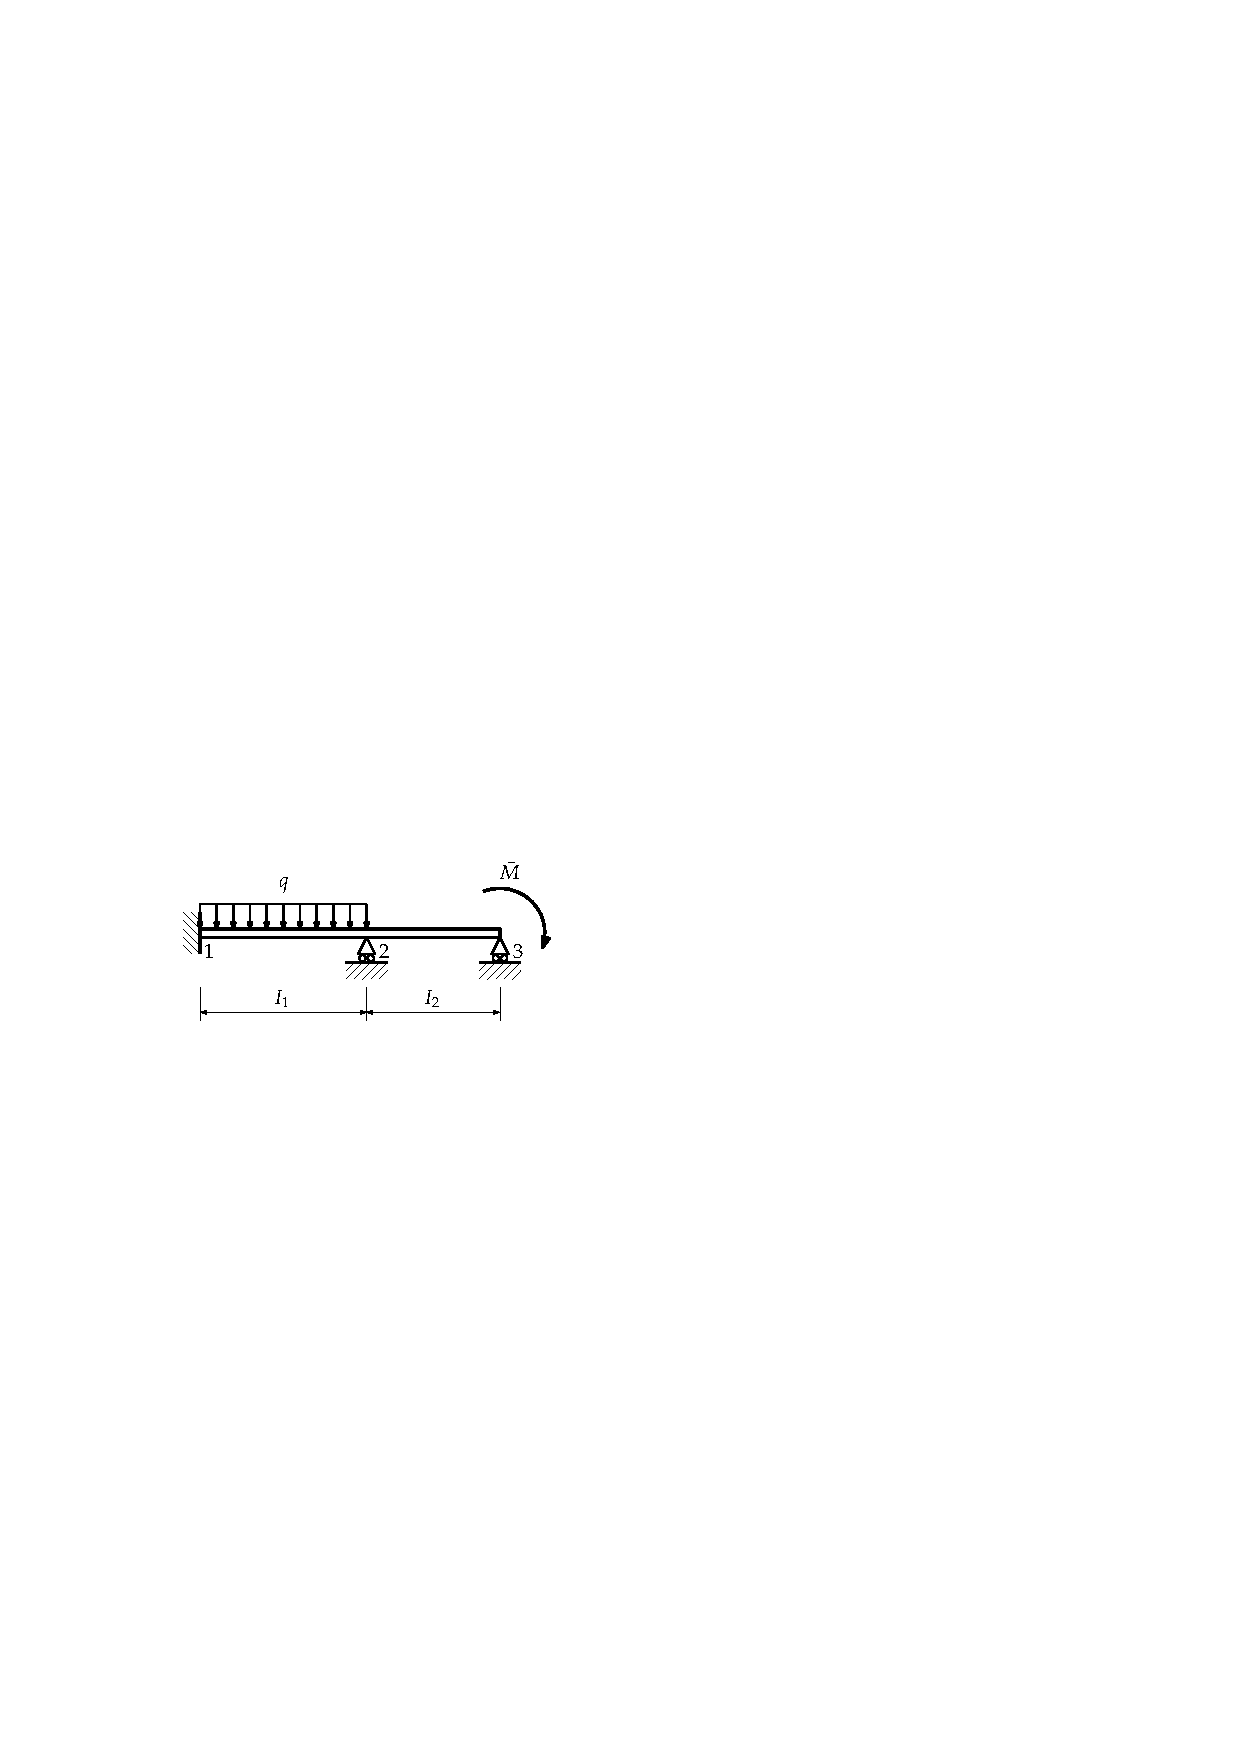
\includegraphics[scale=1.1]{figures/beam_example}
   \caption{2D beam example}
   \label{fig:structMechMod:exem1_1}
 \end{figure}





%%% Local Variables:
%%% mode: latex
%%% TeX-master: "manual"
%%% End:


}{}

\IfFileExists{manual-heattransfermodel.tex}{\chapter{Heat Transfer model}

The heat transfer model is a specific implementation of the \code{Model} interface
dedicated to handle the dynamic heat equation. 
\section{Theory}
The strong form of the dynamic heat equation 
can be expressed as
\begin{equation}
  \rho c_v \dot{T} + \nabla \cdot \vec{\kappa} \nabla T = b
\end{equation}
, with $T$ the temperature scalar field,
$c_v$ the specific heat capacity, 
$\rho$ the mass density, 
$\mat{\kappa}$ the conductivity tensor, and $b$ the heat generation per unit of volume. 
The discretized weak form with the finite number of elements is
\begin{equation}
  \forall i \quad 
  \sum_j \left( \int_\Omega \rho c_v N_j N_i  d\Omega \right) \dot{T}_j 
  - \sum_j \left( \int_\Omega \vec{\kappa} \nabla N_j \nabla N_i d\Omega \right) T_j = 
  - \int_{\Gamma}  N_i \vec{q} \cdot \vec{n} d\Gamma + \int_\Omega b N_i d\Omega
\end{equation}
with $i$ and $j$ the node indices, $\vec{n}$ the normal field to the surface 
$\Gamma = \partial \Omega$. 
To simplify, we can define the capacity and the conductivity matrices as
\begin{equation}
  C_{ij} = \int_\Omega \rho c_v N_j N_i  d\Omega \qquad \textrm{and} \qquad   
  K_{ij} = - \int_\Omega \vec{\kappa} \nabla N_j \nabla N_i d\Omega
\end{equation}
, and the system to solve can be written
\begin{equation}
  \mat{C} \cdot \vec{\dot{T}} = \vec{Q}^{\text{ext}} -\mat{K} \cdot \vec{T}~, 
\end{equation}
with $\vec{Q}^{\text{ext}}$ the consistent heat generated.
\section{Using the heat transfer model}
Currently, the \code{HeatTransferModel} object uses an explicit dynamic analysis.
It can simply be created like this
\begin{cpp}
  HeatTransferModel model(mesh, spatial_dimension);
\end{cpp}
, while an existing mesh has been used (see \ref{sect:common:mesh}).
Then the model object can be initialized with:
\begin{cpp}
  model.initFull("material.dat")
\end{cpp}
, where a material file name has to be provided. This function will load the material 
properties, and allocate / initialize the nodes and element vectors.
More precisely, the heat transfer model contains 4 \code{Vectors}:
\begin{description}
\item[temperature] contains the nodal temperature $T$ (zero  by   default  after  the
  initialization). 
\item[temperature\_rate] contains the variations of temperature $\dot{T}$ 
  (zero  by   default  after  the
  initialization). 
%\item[boundary]  contains a  \code{bool} value for  each  node
%  specifying  whether  temperature is  fixed  or  not. A  Dirichlet  boundary
%  condition can be prescribed by setting the \textbf{boundary} value of a node 
%  to  \code{true}.  A Neumann boundary condition  can only be applied
%  if the  \textbf{boundary} value of a node is  \code{false}. If a
%  node has a  \textbf{boundary} value  that is  \code{false}, the
%  \textbf{temperature},     \textbf{temperature\_rate} and
%  \textbf{residual} are computed by the solve algorithm when relevant\todo{wait for till correction}, 
%  otherwise these  vectors  contain   the  imposed  values.

\item[boundary] contains a  Boolean value for each degree  of freedom specifying
  whether the degree  is blocked or not. A Dirichlet  boundary condition can be
  prescribed by  setting the \textbf{boundary} value  of a degree  of freedom to
  \code{true}.   A Neumann  boundary condition  can  be applied  by setting  the
  corresponding     \textbf{boundary}     value     to    \code{false}.      The
  \textbf{temperature} and  the \textbf{temperature\_rate} are  computed for all
  degrees  of  freedom  where  the  \textbf{boundary}  value   is  set  to
  \code{false}.  For the remaining degrees  of freedom, the imposed values (zero
  by default after  initialization) are kept.

\item[residual] contains the difference between external and internal heat generations. 
The \textbf{residual} contains the supported heat reactions ($\vec{R} = \vec{Q^{ext}} -\mat{K} \cdot \vec{T}$) on
  the nodes that the temperature imposed.
\end{description}

Only a single material can be specified on the domain. 
A material text file (\eg material.dat) provides the material properties as follows:
\begin{cpp}
  heat %\emph{name\_material}% [
  capacity = %\emph{XXX}%
  density = %\emph{XXX}%
  conductivity = [%\emph{XXX}% ... %\emph{XXX}%]
  ]
\end{cpp}
where the \code{capacity} and \code{density} are scalars, and the \code{conductivity} is specified as a $3\times 3$ tensor.

\subsection{Explicit dynamic}

The explicit  time integration scheme in \akantu  uses a lumped capacity
matrix $\mat{C}$ (reducing the computational  cost, see Chapter \ref{sect:smm}). 
This matrix is assembled by
distributing the capacity of each element onto its nodes. Therefore, the resulting $\mat{C}$ is a diagonal matrix stored in the \code{capacity} vector of the model.

\begin{cpp}
  model.assembleCapacityLumped();
\end{cpp}
\index{HeatTransferModel!assembleCapacityLumped}

\note{Currently, only the explicit time integration with lumped capacity matrix 
is implemented within \akantu.} \\

The explicit integration scheme is a \index{Forward Euler} {\it Forward Euler} 
\cite{curnier92a}.

\begin{itemize}
\item Predictor: $\vec{T}_{n+1} = \vec{T}_{n} + \Delta t \dot{\vec{T}}_{n}$
\item Update residual: $\vec{R}_{n+1} = \left( \vec{Q^{ext}_{n+1}} - \vec{K}\vec{T}_{n+1} \right)$
\item Corrector : $\dot{\vec{T}}_{n+1} = \mat{C}^{-1} \vec{R}_{n+1}$
\end{itemize}

The explicit integration scheme is conditionally stable. The time step has to be smaller than the stable time step, 
and it can be obtained in \akantu as follows:

\begin{cpp}
  time_step = model.getStableTimeStep();
\end{cpp}
\index{HeatTransferModel!StableTimeStep}

The stable time step is defined as:
\begin{equation}\label{eqn:htm:explicit:stabletime}
  \Delta t_{\st{crit}} = 2 \Delta x^2 \frac{\rho c_v}{\mid\mid \mat{\kappa} \mid\mid^\infty}
\end{equation}
where $\Delta  x$ is the characteristic length (\eg  the inradius in the  case of
linear triangle  element), $\rho$ is the density, $\mat{\kappa}$ is the conductivity tensor,
and $c_v$ is the specific heat capacity. It is
necessary to impose a time step which is smaller than the stable time step, for
instance, by  multiplying the stable time  step by a safety  factor smaller than
one.

\begin{cpp}
  const Real safety_time_factor = 0.1;
  Real applied_time_step = time_step * safety_time_factor;
  model.setTimeStep(applied_time_step);
\end{cpp}

%The initial temperature  and temperature\_rate fields are, by default,  equal to zero if
%not given specifically by the user (similar to the SolidMechanicsModel initial conditions
%\ref{sect:smm:initial_condition}).

The following loop  allows, for each time  step, to update the  temperatures, residual and
temperature\_rate  fields  following the previously described integration scheme.

\begin{cpp}
  for (UInt s = 1; (s-1)*applied_time_step < total_time; ++s) {
    model.explicitPred();
    model.updateResidual();
    model.explicitCorr();  
  }
\end{cpp}
\index{HeatTransferModel!explicitPred}
\index{HeatTransferModel!explicitCorr}
\index{HeatTransferModel!updateResidual}
\index{HeatTransferModel!solveExplicitLumped}

An    example    of    explicit     dynamic    heat propagation is    presented    in \\
\shellcode{\examplesdir/heat\_transfer/explicit\_heat\_transfer.cc}.  \\
This example  consists of a square 2D plate of \unit{1}{\squaremetre} 
having an initial temperature of \unit{100}{\kelvin} everywhere but a none centered hot point 
maintained at \unit{300}{\kelvin}. Figure \ref{fig:htm:explicit:dynamic} presents the
geometry of this case. The material used is a linear fictitious elastic material
with  a density  of  \unit{8940}{\kilogrampercubicmetre}, a  conductivity of 
\unit{401}{\watt\per\metre\per\kelvin} and a specific heat capacity of \unit{385}{\joule\per\kelvin\per\kilogram}. The time step used is \unit{0.12}{\second}.

\begin{figure}[!htb]
  \centering
  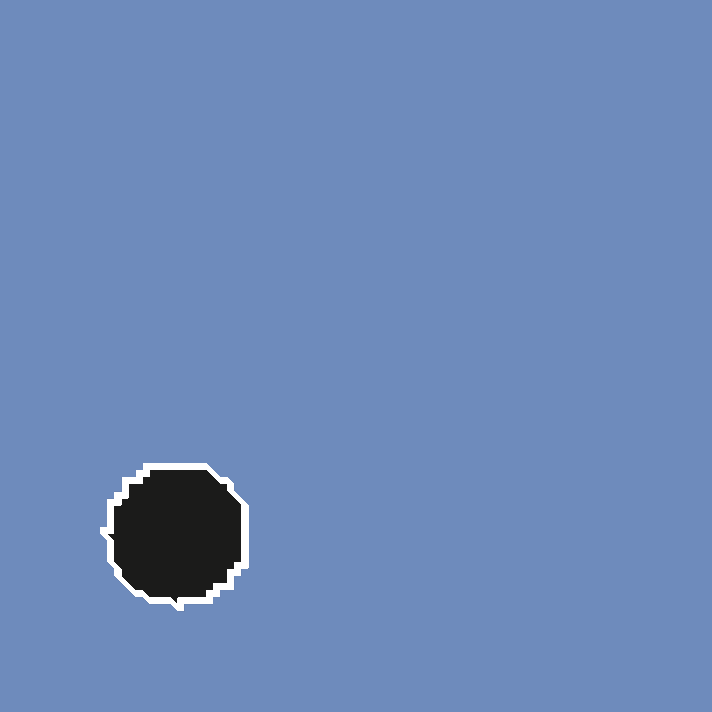
\includegraphics[width=.4\textwidth]{figures/hot-point-1}
  \hfill
  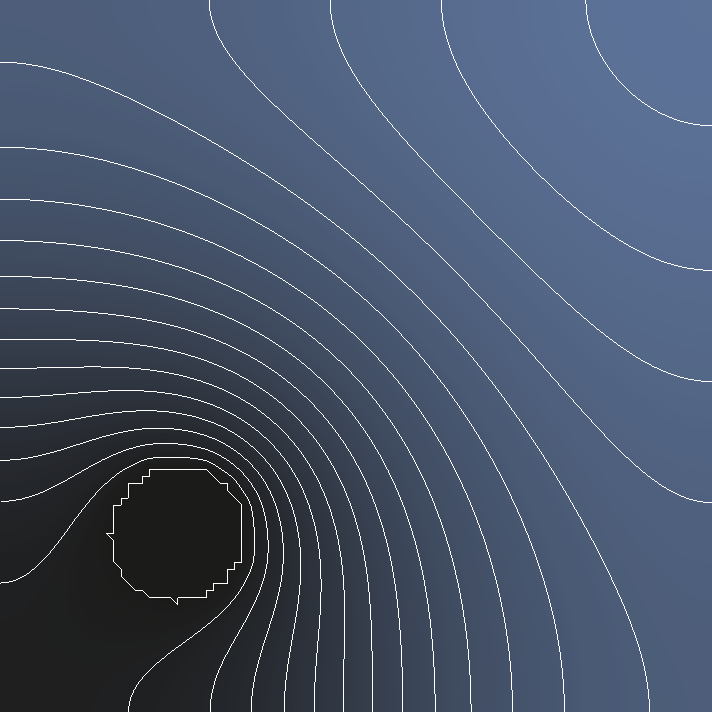
\includegraphics[width=.4\textwidth]{figures/hot-point-2}
  \caption{Initial temperature field (left) and after 15000 time steps = 30 minutes (right). The lines represent iso-surfaces.}
  \label{fig:htm:explicit:dynamic}
\end{figure}

}{}

\chapter{Input/output}\index{I\/O}

In this chapter the problem of getting the internal data in a human readable way
willl be expressed. The models in \akantu handles the data associated to your
mesh, but this data can be splitted in many \code{Vectors}. For examples the
data stored per element type in a \code{ByElementTypeVector} are composed by as
many vectors as types in the mesh.

To help you to get this data in a visualization software, the models contains a
object to dump \code{VTK} files. This files can be visualized in software such
as \code{ParaView}, \code{ViSit} or \code{Mayavi}.

The internal dumper of the model can be configured to specify which data field
need to be output. This is done with the
\code{addDumpField}\index{I\/O!addDumpField} method. By default all the files are
generated in a folder call \code{paraview/}

\begin{cpp}
  model.setBaseName("output"); // prefix for all generated files

  model.addDumpField("displacement");
  model.addDumpField("stress");
  ...

  model.dump()
\end{cpp}

The fields are dumped with the number of component they have in the memory, that
is to say that for example in 2D vectors have 2 components and $2^{nd}$ order
tensors have $2\times2$ component.  This can be changed by using
\code{addDumpFieldVector}\index{I\/O!addDumpFieldVector} which always dumps
vectors with 3 components or
\code{addDumpFieldTensor}\index{I\/O!addDumpFieldTensor} which dumps $2^{nd}$
order tensors with $3\times3$ components.

The field which are stored by quadrature points are modified to be seen in the
\code{VTK} file as elemental data. to do this the default is to average the
values of the quadrature points.

The list of fields depends on the models.

\paragraph{\code{SolidMechanicsModel}:\index{I\/O!SolidMechanicsModel}}\hfill
\vspace*{0.2cm}

\begin{tabular}{llll}
  \toprule
  key          &    type      & support \\
  \midrule
  displacement & Vector<Real> & nodes  \\
  velocity     & Vector<Real> & nodes  \\
  acceleration & Vector<Real> & nodes  \\
  force	     & Vector<Real> & nodes  \\
  residual     & Vector<Real> & nodes  \\
  boundary     & Vector<bool> & nodes  \\
  mass         & Vector<Real> & nodes  \\
  partitions   & Real         & elements \\
  stress & Matrix<Real> & quadrature points  \\
  strain & Matrix<Real> & quadrature points  \\
  \textit{material internals} & variable  & quadrature points  \\
\bottomrule
\end{tabular}


The user can also register external fields which have the same mesh as the mesh from the model as support. To do this an object of type \code{Field} as to be created.\index{I\/O!addDumpFieldExternal}

\begin{itemize}
\item For nodal fields :
\begin{cpp}
  Vector<T> vect(nb_nodes, nb_component);
  Field field = new DumperIOHelper::NodalField<T>(vect));
  model.addDumpFieldExternal("my_field", field);
\end{cpp}

\item For elemental fields :
\begin{cpp}
  ByElementTypeVector<T> vect;
  Field field = new DumperIOHelper::ElementalField<T>(vect, spatial_displacement));
  model.addDumpFieldExternal("my_field", field);
\end{cpp}
\end{itemize}

\IfFileExists{manual-parallel.tex}{\chapter{Parallel Computation}

This section explains how to launch a parallel computation.
The strategy adopted by \akantu uses a mesh partitioning
where elements are mapped to processors. Mesh partitions are
then distributed to available processors by adequate routines
as will be described below.
The sequence of additional operations to be performed by the user are:

\begin{itemize}
\item Initializing the parallel context
\item Partitioning the mesh
\item Distributing mesh partitions
\end{itemize}

After these steps, the \code{Model}
object proceeds with the interprocess communication automatically
without the user having to explicitly take care of them.
In what follows we show how it works on a \code{SolidMechanics} model.

\section{Initializing the Parallel Context}

The user must initialize \akantu by forwarding the arguments passed to the
program by using the function \code{initialize}, and close \akantu instances
at the end of the program by calling the \code{finalize} function.

\note{This step does not change from the sequential case as it was stated in
Section \ref{sect:common:main}. It only gives a additional motivation in the parallel/MPI context.}

The \code{initialize} function builds a \code{StaticCommunicator} object
responsible for handling the interprocess communications later on.  The
\code{StaticCommunicator} can, for instance, be used to ask the total number of
declared processors available for computations as well as the process rank
through the functions \code{getNbProc} and \code{whoAmI} respectively.

An example of the initializing sequence and basic usage of the
\code{StaticCommunicator} is:

\begin{cpp}
int main(int argc, char *argv[]) {
  initialize("material.dat", argc, argv);

  const auto & comm = Communicator::getWorldCommunicator();
  Int psize = comm.getNbProc();
  Int prank = comm.whoAmI();

  ...

  finalize();
}
\end{cpp}

\section{Partitioning and distributing the Mesh}

The mesh is partitioned after the correct initialization of the processes
playing a role in the computation. We assume that a \code{Mesh} object is
constructed as presented in Section~\ref{sect:common:mesh}.  Then it can be
distributed among the different processes. At the moment, the only partitioner
available is \code{MeshPartitionScotch} which is used by the function
\code{distribute} using the \textbf{Scotch}\cite{scotch} program.  This is
achieved by the following code:

\begin{cpp}
  Mesh mesh(spatial_dimension);
  if(prank == 0) {
    mesh.read("my_mesh.msh");
  }
  mesh.distribute();
\end{cpp}

The algorithm that partition the mesh needs the generation of a random
distribution of values. Therefore, in order to run several time a
simulation with the same partition of the mesh, the \emph{seed} has to
be set manually.  This can be done either by adding the following line
to the input file \emph{outside} the material parameters environments:
\begin{cpp}
  seed = 1
\end{cpp}
where the value 1.0 can be substituted with any number, or by setting
it directly in the code with the command:
\begin{cpp}
  RandGenerator:: seed(1)
\end{cpp}
The latter command, with empty brackets, can be used to check the value
of the \emph{seed} used in the simulation.

\note{Only the processor of rank $0$ should load the mesh file to
  partition it. Nevertheless, the \code{Mesh} object must by declared
  for all processors since the mesh distribution will store mesh pieces to that object.}

An example of an explicit dynamic 2D bar in compression in a parallel
context can be found in \shellcode{\examplesdir/parallel\_2d}.

\section{Launching a Parallel Program}

Using \textbf{MPI} a parallel run can be launched from a shell
using the command

\begin{cpp}
  mpirun -np #procs program_name parameter1 parameter2 ...
\end{cpp}

%%% Local Variables:
%%% mode: latex
%%% TeX-master: "manual"
%%% End:
}{}

\IfFileExists{manual-contact.tex}{

\chapter{Contact}

\section{Implicit Contact Solver}

The contact formulation corresponds to the augmented-Lagrangian method \cite{Laursen:2002}, which seeks to minimize the following energy functional between two bodies with contact interface $ \Gamma_c^{\left( 1 \right)} $:
\begin{equation} \label{eq:functinal}
  \Pi^{al} \left( \boldsymbol u, \lambda_N \right) := \sum_{i=1}^2 \Pi ^{\left( i \right) } ( \boldsymbol u ^{\left( i \right) }  ) + \int_{\Gamma_c^{\left( 1 \right) } } \left[ \frac{1}{2 \epsilon_N } \left< \lambda_N + \epsilon_N g \right>^ 2 - \frac{1}{2 \epsilon_N} \lambda^2_N \right] \, d\Gamma,
\end{equation}
where $ \Pi^{\left( i \right) } $ corresponds to the energy functional of the $ i $-th body in contact, which is a function of the displacement field $\boldsymbol u$ and the Lagrangian multiplier $\lambda_N$. In the equation above, $\epsilon_N$ is a penalty parameter,  $g$ the contact gap function, and $\left< \cdot \right>$ the Macaulay bracket.

The solution procedure seeks to make the equation above stationary with respect to both $\boldsymbol u$ and $\lambda_N$:
\begin{equation}
\begin{aligned}
 0 &= D_{\boldsymbol u} \Pi^{al} \cdot \boldsymbol w = G^{int,ext} \left( \boldsymbol u, \boldsymbol w \right) + \int_{\Gamma_c^{\left( 1 \right) } } \left< \lambda_N + \epsilon_N g \right> \delta g  \, d\Gamma  \qquad  \forall \boldsymbol w \in \mathcal{V} \\
0 &= D_{ \lambda} \Pi^{al} \cdot q_N  = \frac{1}{\epsilon_N} \int_{\Gamma_c^{\left( 1 \right) } } \left[ \left< \lambda_N + \epsilon_N g \right> - \lambda_N \right] q_N  \, d\Gamma  \qquad  \forall q_N \in \mathcal{M}
\end{aligned}
\end{equation}

A solution is then found by using Uzawa's method, for which we solve for $ \boldsymbol u ^ {\left( k \right) }$, with $ \lambda_N^{\left( k \right)}$ fixed:
\begin{equation}
 G^{int,ext} ( \boldsymbol u ^ {\left( k \right) }, \boldsymbol w ) + \int_{\Gamma_c^{\left( 1 \right) } } \left< \lambda_N^ {\left( k \right) } + \epsilon_N g( \boldsymbol u ^ {\left( k \right) } )  \right> \delta g  \, d\Gamma = 0 \qquad \forall \boldsymbol w \in \mathcal{V},
 \end{equation}

followed by an update of the multipliers on $\Gamma_c ^ {\left( 1 \right) }$:
\begin{equation}
\lambda _N ^ {\left( k+1 \right) } = \left< \lambda_N ^ {\left( k \right) } + \epsilon_N g ( \boldsymbol u ^ {\left( k \right) } ) \right>.
\end{equation}


It is worth noting that the results of the implicit contact resolution depend largely on the choice of the penalty parameter $ \epsilon_N $. Depending on this parameter, the computational time needed to obtain a converged solution can be increased dramatically, or a convergence solution could not even be obtained at all.

The code provides a flag that allows the user to rely on an automatic value of $ \epsilon_N $ for each slave node. Yet, this value should be used as a reference only, since for some problems it is actually overestimated and convergence cannot be obtained.


\subsection{Implementation}

In \akantu, the object that handles the implicit contact can be found in \code{implicit\_contact\_manager.hh}.
The object that handles the implicit contact resolution stage is the class template
\begin{cpp}
template <int dim, class model_type> struct ContactData;
\end{cpp}
This object takes the command line parameters during construction, which can be used to set up the behavior during contact resolution. The object can take the following parameters (default values in brackets):

\begin{tabular}{lrl}
  -e & [auto] & Penalty parameter for augmented-Lagrangian formulation \\
  -alpha & [1] & Multiplier for values of the penalty parameter\\
 -utol & [0.001] & Tolerance used for multipliers in the Uzawa method\\
 -ntol &[0.001]& Tolerance used in the Newton-Raphson inner convergence loop\\
 -usteps &[100]&  Maximum number of steps allowed in the Uzawa loop\\
 -nsteps & [100]&  Maximum number of steps allowed in the Newton-Raphson loop\\
\end{tabular} \\


Also, the following flags can be given to the command line


\begin{tabular}{ll}
 -dump&          Dumping within Newton iterations \\
 -v&             Verbose output
\end{tabular} \\



The \code{ContactData} object stores the state of the contact mechanics simulation. The state is contained within the following variables:

\begin{tabular}{ll}
 \code{sm\_}  & slave-master map \\
 \code{multipliers\_} & Lagrange multiplier map \\
 \code{areas\_} & slave areas map \\
 \code{penalty\_} & penalty parameter map \\
 \code{gaps\_} & gap function map \\
 \code{model\_} & reference to solid mechanics model \\
 \code{multiplier\_dumper\_} & structures used to dump multipliers \\
  \code{pressure\_dumper\_} & structures used to dump pressure \\
 \code{options\_} & options map \\
 \code{flags\_} & flags map \\
 \code{uiter\_}, \code{niter\_} & Uzawa and Newton iteration counters
\end{tabular} \\


The interface of the \code{ContactData} object contains three methods to solve for each contact step, which is overloaded depending on the parameters passed. Their signatures are as follows


\begin{cpp}
void solveContactStep();

void solveContactStep(search_type *search);

template <class PostAssemblyFunctor>
void solveContactStep(search_type *search, const PostAssemblyFunctor& fn);
}
\end{cpp}

The second method allows the user to provide a pointer to an object that is used to search slave-master pairs. This can be done, for example, when due to the deformed configuration current slave-master pairs are no longer valid.
The last method in the snippet above allows the user to provide a functor that is called after the assembly of the contact contributions to the stiffness matrix and the force vector. The last takes place within the method \code{computeTangentAndResidual()}.


\subsubsection{Hertz Example}


Here we outline, step by step, the use of the implicit contact solver to obtain the solution of Hertzian contact. The complete implementation can be found in \code{examples/contact/hertz\_3D.cc}.

The following class is used as the object that will perform the search for new contact elements when a slave node is found to lie outside its master element. The class derives from a \code{SearchBase} class, and implements the virtual method \code{search}.

\begin{cpp}
struct Assignator : public ContactData<3,SolidMechanicsModel>::SearchBase {
  typedef Point <3> point_type;
  typedef SolidMechanicsModel model_type;
  typedef ModelElement <model_type> master_type;

  model_type &model_;

  Assignator(model_type& model) : model_(model) {}

  virtual int search(const Real *ptr) {
    point_type p(ptr);

    ElementGroup &rs = model_.getMesh().getElementGroup("rigid_surface");

    for (ElementGroup::type_iterator tit = rs.firstType(); tit != rs.lastType(); ++tit)
      for (ElementGroup::const_element_iterator it = rs.element_begin(*tit);
           it != rs.element_end(*tit); ++it) {
        master_type m(model_, _triangle_3, *it);
        if (point_has_projection_to_triangle(p, m.point <3>(0), m.point <3>(1), m.point <3>(2))) {
          return m.element;
        }
      }
    return -1;
  }
};
\end{cpp}


The first thing we do in the main file is to add some type definitions:

\begin{cpp}

int main(int argc, char *argv[]) {

  // set dimension
  static const UInt dim = 3;

  // type definitions
  typedef Point <dim> point_type;
  typedef BoundingBox <dim> bbox_type;
  typedef SolidMechanicsModel model_type;
  typedef ModelElement <model_type> master_type;
  typedef ContactData <dim, model_type> contact_type;

  typedef std::chrono::high_resolution_clock clock;
  typedef std::chrono::seconds seconds;
\end{cpp}

We initialize the library, create a mesh, and set the solid mechanics model up:

\begin{cpp}

  initialize("steel.dat", argc, argv);

  // create mesh
  Mesh mesh(dim);

  // read mesh
  mesh.read("hertz_3D.msh");

  // create model
  model_type model(mesh);
  SolidMechanicsModelOptions opt(_static);

  // initialize material
  model.initFull(opt);
\end{cpp}


Then we create the contact data, which can be used to solve the contact problem. Note that some of the parameters required by the contact object can be coded in the implementation file (these can also be passed as arguments).
\begin{cpp}

  // create data structure that holds contact data
  contact_type cd(argc, argv, model);

  // optimal value of penalty multiplier
  cd[Alpha] = 0.05;
  cd[Uzawa_tol] = 1.e-2;
  cd[Newton_tol] = 1.e-2;
\end{cpp}


Next we find the area that corresponds to each slave node. For this we use the fact that if we apply a unit distributed load over the contact surface, the resulting force vector at each slave node has magnitude that is equal to the area.
\begin{cpp}

  // get physical names from Gmsh file
  mesh.createGroupsFromMeshData <std::string>("physical_names");

  // get areas for the nodes of the circle
  // this is done by applying a unit pressure to the contact surface elements
  model.applyBC(BC::Neumann::FromHigherDim(Matrix <Real>::eye(3, 1.)), "contact_surface");
  Array <Real>& areas = model.getForce();

  // loop over contact surface nodes and store node areas
  ElementGroup &eg = mesh.getElementGroup("contact_surface");
  cout << "- Adding areas to slave nodes. " << endl;
  for (auto nit = eg.node_begin(); nit != eg.node_end(); ++nit) {
    // compute area contributing to the slave node
    Real a = 0.;
    for (UInt i = 0; i < dim; ++i)
      a += pow(areas(*nit, i), 2.);
    cd.addArea(*nit, sqrt(a));
  }

  // set force value to zero
  areas.clear();
\end{cpp}

Note that we clear the force vector after the assignment of areas.

In the next step we prescribe the boundary conditions that do not change in time:

\begin{cpp}

  // apply boundary conditions for the rigid plane
  model.applyBC(BC::Dirichlet::FixedValue(0., BC::_x), "bottom_body");
  model.applyBC(BC::Dirichlet::FixedValue(0., BC::_y), "bottom_body");
  model.applyBC(BC::Dirichlet::FixedValue(0., BC::_z), "bottom_body");

  // block z-disp in extreme points of top surface
  model.getBoundary()(1, 2) = true;
  model.getBoundary()(2, 2) = true;

  // block x-disp in extreme points of top surface
  model.getBoundary()(3, 0) = true;
  model.getBoundary()(4, 0) = true;

\end{cpp}


Next we add the slave-master pairs for the analysis. We use a bounding box to consider only a fraction of the slave nodes in the model. Those slave nodes that are not within the bounding box are not considered in the analysis:
\begin{cpp}

  // set-up bounding box to include slave nodes that lie inside it
  Real l1 = 1.;
  Real l2 = 0.2;
  Real l3 = 1.;
  point_type c1(-l1 / 2, -l2 / 2, -l3 / 2);
  point_type c2(l1 / 2,  l2 / 2,  l3 / 2);
  bbox_type bb(c1, c2);

  // search policy for slave-master pairs
  Assignator a(model);


  // loop over nodes in contact surface to create contact elements
  cout << "- Adding slave-master pairs" << endl;
  for (auto nit = cs.node_begin(); nit != cs.node_end(); ++nit) {
    point_type p(&coords(*nit));

    // ignore slave node if it doesn't lie within the bounding box
    if (!(bb & p))
      continue;

    int el = a.search(&coords(*nit));
    if (el != -1)
      cd.addPair(*nit, master_type(model, _triangle_3, el));
  }
\end{cpp}


We then start the loop over displacement increments, and at each step we call {{{solveContactStep}}} and save the displacement, resulting force, and maximum pressure, in an array that will be used to print the results at the end of the simulation:
\begin{cpp}

  const size_t steps = 30;
  Real data[3][steps]; // store results for printing
  Real step = 0.001;  // top displacement increment
  size_t k = 0;

  for (Real delta = 0; delta <= step * steps; delta += step) {
    // apply displacement to the top surface of the half-sphere
    model.applyBC(BC::Dirichlet::FixedValue(-delta, BC::_y), "top_surface");

    // solve contact step, this method also dumps Paraview files
    cd.solveContactStep(&a);

    data[0][k] = delta;
    data[1][k] = cd.getForce();
    data[2][k] = cd.getMaxPressure();
    ++k;
  }
\end{cpp}


The last portion of the output of code above is as follows:
\begin{verbatim}
         Disp.         Force  Max pressure
             0             0             0
         0.001          1.29     6.068e+04
         0.002     6.702e+06      6.78e+09
         0.003     1.832e+07     9.453e+09
         0.004     3.349e+07     1.091e+10
         0.005       5.2e+07     1.171e+10
         0.006     7.211e+07     1.298e+10
         0.007     9.377e+07     1.481e+10
         0.008     1.183e+08     1.624e+10
         0.009      1.41e+08     1.616e+10
          0.01       1.7e+08     1.688e+10
         0.011     1.963e+08     1.678e+10
         0.012     2.263e+08     1.758e+10
         0.013     2.581e+08     1.805e+10
         0.014     2.907e+08     1.821e+10
         0.015     3.244e+08     1.877e+10
         0.016     3.593e+08     1.954e+10
         0.017     4.051e+08     2.131e+10
         0.018     4.317e+08     2.115e+10
         0.019     4.823e+08     2.201e+10
          0.02     5.237e+08     2.315e+10
         0.021     5.639e+08     2.379e+10
         0.022     6.058e+08     2.405e+10
         0.023     6.483e+08     2.485e+10
         0.024     6.917e+08     2.536e+10
         0.025     7.363e+08     2.854e+10
         0.026     7.681e+08     3.099e+10
         0.027     8.332e+08     3.291e+10
         0.028     8.577e+08     3.399e+10
         0.029     9.281e+08     3.426e+10
\end{verbatim}

The following figure shows the deformed state of the half-sphere at the end of the simulation, together with the contact pressure distribution:

\begin{figure}[htbp]
\begin{center}
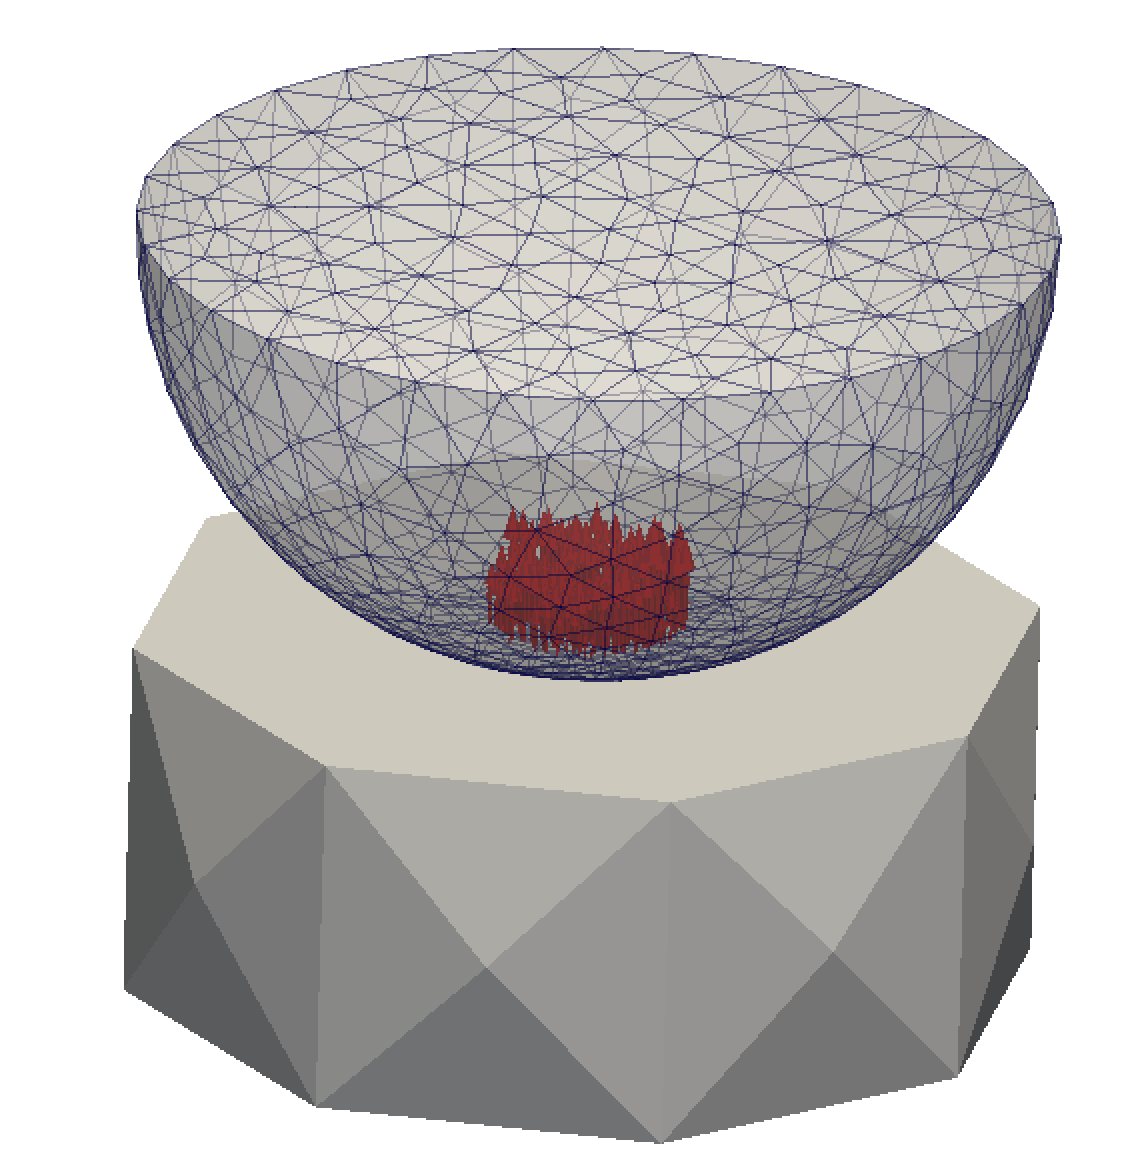
\includegraphics[scale=0.3]{figures/hertz_3D.png}
\caption{State of pressure and deformation at the end of the simulation of the example of Hertz in 3D.}
\label{fig:hertz_3D}
\end{center}
\end{figure}
}{}


% The appendices
\appendix
\chapter{Shape Functions\index{Elements}}
\label{app:elements}
Schmatic overview of all the element types defined in \akantu is described in Chapter~\ref{chap:elements}. In this appendix, more detailed information (shape function, location of Gaussian quadrature points, and so on) of each of these types is listed. For each element type, the coordinates of the nodes are given in the isoparametric frame of reference, together with the shape functions (and their derivatives) on these respective nodes. Also all the Gaussian quadrature points within each element are assigned (together with the weight that is applied on these points). The graphical representations of all the element types can be found in Chapter~\ref{chap:elements}.

%%%%%%%%%% 1D %%%%%%%%%
%\section{Isoparametric Elements in 1D\index{Elements!1D}}
\section{1D-Shape Functions\index{Elements!1D}}
\subsection{Segment 2\index{Elements!1D!Segment 2}}

\begin{Element}{1D}
 1  &  \inelemone{-1}  &  $\half\left(1-\xi\right)$  &  \inelemone{-\half} \\
\elemline
 2  &  \inelemone{1}   &  $\half\left(1+\xi\right)$  &  \inelemone{\half}  \\
\end{Element}

\begin{QuadPoints}{lc}
Coord. \elemcooroned  &  0  \\
\elemline
Weight  &  2  \\
\end{QuadPoints}

\subsection{Segment 3\index{Elements!1D!Segment 3}}

\begin{Element}{1D}
 1  &  \inelemone{-1}  &  $\half\xi\left(\xi-1\right)$  &  \inelemone{\xi-\half}   \\
\elemline
 2  &  \inelemone{1}   &  $\half\xi\left(\xi+1\right)$  &  \inelemone{\xi+\half}   \\
\elemline
 3  &  \inelemone{0}   &  $1-\xi^{2}$                    &  \inelemone{-2\xi}       \\
\end{Element}

\begin{QuadPoints}{lcc}
Coord. \elemcooroned  &  $-1/\sqrt{3}$  &  $1/\sqrt{3}$  \\
\elemline
Weight  &  1  &  1  \\
\end{QuadPoints}

%%%%%%%%%% 2D %%%%%%%%%
%\section{Isoparametric Elements in 2D\index{Elements!2D}}
\section{2D-Shape Functions\index{Elements!2D}}
\subsection{Triangle 3\index{Elements!2D!Triangle 3}}

\begin{Element}{2D}
 1  &  \inelemtwo{0}{0}  &  $1-\xi-\eta$  &  \inelemtwo{-1}{-1}  \\
\elemline
 2  &  \inelemtwo{1}{0}  &  $\xi$         &  \inelemtwo{1}{0}    \\
\elemline
 3  &  \inelemtwo{0}{1}  &  $\eta$        &  \inelemtwo{0}{1}    \\
\end{Element}

\begin{QuadPoints}{lc}
Coord. \elemcoortwod  &  \inquadtwo{\third}{\third}  \\
\elemline
Weight  &  1  \\
\end{QuadPoints}

\subsection{Triangle 6\index{Elements!2D!Triangle 6}}

\begin{Element}{2D}
 1  &  \inelemtwo{0}{0}          &  $-\left(1-\xi-\eta\right)\left(1-2\left(1-\xi-\eta\right)\right)$ & \inelemtwo{1-4\left(1-\xi-\eta\right)}{1-4\left(1-\xi-\eta\right)} \\
\elemline
 2  &  \inelemtwo{1}{0}          &  $-\xi\left(1-2\xi\right)$                                         & \inelemtwo{4\xi-1}{0}                          \\
\elemline
 3  &  \inelemtwo{0}{1}          &  $-\eta\left(1-2\eta\right)$                                       & \inelemtwo{0}{4\eta-1}                   \\
\elemline
 4  &  \inelemtwo{\half}{0}      &  $4\xi\left(1-\xi-\eta\right)$                                     & \inelemtwo{4\left(1-2\xi-\eta\right)}{-4\xi}                      \\
\elemline
 5  &  \inelemtwo{\half}{\half}  &  $4\xi\eta$                                                        & \inelemtwo{4\eta}{4\xi}                       \\
\elemline
 6  &  \inelemtwo{0}{\half}      &  $4\eta\left(1-\xi-\eta\right)$                                    & \inelemtwo{-4\eta}{4\left(1-\xi-2\eta\right)}  \\
\elemline
\end{Element}

\begin{QuadPoints}{lccc}
Coord. \elemcoortwod  &  \inquadtwo{\sixth}{\sixth} & \inquadtwo{\twothird}{\sixth} & \inquadtwo{\sixth}{\twothird} \\
\elemline
Weight & \sixth & \sixth & \sixth \\
\end{QuadPoints}
\clearpage

\subsection{Quadrangle 4\index{Elements!2D!Quadrangle 4}}

\begin{Element}{2D}
 1  &  \inelemtwo{-1}{-1}  &  $\quart\left(1-\xi\right)\left(1-\eta\right)$  &  \inelemtwo{-\quart\left(1-\eta\right)}{-\quart\left(1-\xi\right)} \\
\elemline
 2  &  \inelemtwo{1}{-1}   &  $\quart\left(1+\xi\right)\left(1-\eta\right)$  &  \inelemtwo{\quart\left(1-\eta\right)}{-\quart\left(1+\xi\right)} \\
\elemline
 3  &  \inelemtwo{1}{1}    &  $\quart\left(1+\xi\right)\left(1+\eta\right)$  &  \inelemtwo{\quart\left(1+\eta\right)}{\quart\left(1+\xi\right)}  \\
\elemline
 4  &  \inelemtwo{-1}{1}   &  $\quart\left(1-\xi\right)\left(1+\eta\right)$  &  \inelemtwo{-\quart\left(1+\eta\right)}{\quart\left(1-\xi\right)}  \\
\end{Element}

\begin{QuadPoints}{lcccc}
\elemcoortwod  &  \inquadtwo{-\invsqrtthree}{-\invsqrtthree}  &  \inquadtwo{\invsqrtthree}{-\invsqrtthree}  
               &  \inquadtwo{\invsqrtthree}{\invsqrtthree}    &  \inquadtwo{-\invsqrtthree}{\invsqrtthree} \\ 
\elemline
Weight & 1 & 1 & 1 & 1 \\
\end{QuadPoints}

\subsection{Quadrangle 8\index{Elements!2D!Quadrangle 8}}

\begin{Element}{2D}
 1  &  \inelemtwo{-1}{-1}  &  $\quart\left(1-\xi\right)\left(1-\eta\right)\left(-1-\xi-\eta\right)$ 
                           &  \inelemtwo{\quart\left(1-\eta\right)\left(2\xi+\eta\right)}
                                        {\quart\left(1-\xi\right)\left(\xi+2\eta\right)}  \\
\elemline
 2  &  \inelemtwo{1}{-1}  &  $\quart\left(1+\xi\right)\left(1-\eta\right)\left(-1+\xi-\eta\right)$ 
                          &  \inelemtwo{\quart\left(1-\eta\right)\left(2\xi-\eta\right)}
                                       {-\quart\left(1+\xi\right)\left(\xi-2\eta\right)} \\
\elemline
 3  &  \inelemtwo{1}{1}  &  $\quart\left(1+\xi\right)\left(1+\eta\right)\left(-1+\xi+\eta\right)$ 
                         &  \inelemtwo{\quart\left(1+\eta\right)\left(2\xi+\eta\right)}
                                      {\quart\left(1+\xi\right)\left(\xi+2\eta\right)}  \\
\elemline
 4  &  \inelemtwo{-1}{1}  &  $\quart\left(1-\xi\right)\left(1+\eta\right)\left(-1-\xi+\eta\right)$ 
                          &  \inelemtwo{\quart\left(1+\eta\right)\left(2\xi-\eta\right)}
                                       {-\quart\left(1-\xi\right)\left(\xi-2\eta\right)} \\
\elemline
 5  &  \inelemtwo{0}{-1}  &  $\half\left(1-\xi^{2}\right)\left(1-\eta\right)$ 
                          &  \inelemtwo{-\xi\left(1-\eta\right)}
                                       {-\half\left(1-\xi^{2}\right)}  \\
\elemline
 6  &  \inelemtwo{1}{0}  &  $\half\left(1+\xi\right)\left(1-\eta^{2}\right)$
                         &  \inelemtwo{\half\left(1-\eta^{2}\right)}
                                      {-\eta\left(1+\xi\right)}  \\
\elemline
 7  &  \inelemtwo{0}{1}  &  $\half\left(1-\xi^{2}\right)\left(1+\eta\right)$
                         &  \inelemtwo{-\xi\left(1+\eta\right)}
                                      {\half\left(1-\xi^{2}\right)}  \\
\elemline
 8  & \inelemtwo{-1}{0}  &  $\half\left(1-\xi\right)\left(1-\eta^{2}\right)$
                         &  \inelemtwo{-\half\left(1-\eta^{2}\right)}
                                      {-\eta\left(1-\xi\right)}  \\
\end{Element}

\begin{QuadPoints}{lccccc}
Coord. \elemcoortwod & \inquadtwo{0}{0} & \inquadtwo{\sqrt{\tfrac{3}{5}}}{\sqrt{\tfrac{3}{5}}} & \inquadtwo{-\sqrt{\tfrac{3}{5}}}{\sqrt{\tfrac{3}{5}}} 
                     & \inquadtwo{-\sqrt{\tfrac{3}{5}}}{-\sqrt{\tfrac{3}{5}}} & \inquadtwo{\sqrt{\tfrac{3}{5}}}{-\sqrt{\tfrac{3}{5}}} \\
\elemline
Weight & 64/81 & 25/81 & 25/81 & 25/81 & 25/81 \\
\elemline
Coord. \elemcoortwod & \inquadtwo{0}{\sqrt{\tfrac{3}{5}}} & \inquadtwo{-\sqrt{\tfrac{3}{5}}}{0} 
                     & \inquadtwo{0}{-\sqrt{\tfrac{3}{5}}} & \inquadtwo{\sqrt{\tfrac{3}{5}}}{0} & \\
\elemline
Weight & 40/81 & 40/81 & 40/81 & 40/81 & \\
\end{QuadPoints}
\clearpage
%%%%%%%%%% 3D %%%%%%%%%
\section{3D-Shape Functions\index{Elements!3D}}
%\section{Isoparametric Elements in 3D\index{Elements!3D}}

\subsection{Tetrahedron 4\index{Elements!3D!Tetrahedron 4}}

\begin{Element}{3D}
 1 & \inelemthree{0}{0}{0} & $1-\xi-\eta-\zeta$ & \inelemthree{-1}{-1}{-1} \\
\elemline 
 2 & \inelemthree{1}{0}{0} & $\xi$              & \inelemthree{1}{0}{0} \\
\elemline 
 3 & \inelemthree{0}{1}{0} & $\eta$             & \inelemthree{0}{1}{0} \\
\elemline 
 4 & \inelemthree{0}{0}{1} & $\zeta$            & \inelemthree{0}{0}{1} \\
\end{Element}

\begin{QuadPoints}{lc}
Coord. \elemcoorthreed & \inquadthree{\quart}{\quart}{\quart} \\
\elemline
Weight & \sixth \\
\end{QuadPoints}

\subsection{Tetrahedron 10\index{Elements!3D!Tetrahedron 10}}

\begin{Element}{3D}
  1 & \inelemthree{0}{0}{0} & $\left(1-\xi-\eta-\zeta\right)\left(1-2\xi-2\eta-2\zeta\right)$ 
                            & \inelemthreecolumn{4\xi+4\eta+4\zeta-3}{4\xi+4\eta+4\zeta-3}{4\xi+4\eta+4\zeta-3}\\
\elemline
  2 & \inelemthree{1}{0}{0} & $\xi\left(2\xi-1\right)$
                            & \inelemthree{4\xi-1}{0}{0} \\
\elemline
  3 & \inelemthree{0}{1}{0} & $\eta\left(2\eta-1\right)$
                            & \inelemthree{0}{4\eta-1}{0} \\
\elemline
  4 & \inelemthree{0}{0}{1} & $\zeta\left(2\zeta-1\right)$
                            & \inelemthree{0}{0}{4\zeta-1} \\
\elemline
  5 & \inelemthree{\half}{0}{0} & $4\xi\left(1-\xi-\eta-\zeta\right)$
                                & \inelemthree{4-8\xi-4\eta-4\zeta}{-4\xi}{-4\xi} \\
\elemline
  6 & \inelemthree{\half}{\half}{0} & $4\xi\eta$
                                    & \inelemthree{4\eta}{4\xi}{0} \\
\elemline
  7 & \inelemthree{0}{\half}{0} & $4\eta\left(1-\xi-\eta-\zeta\right)$
                                & \inelemthree{-4\eta}{4-4\xi-8\eta-4\zeta}{-4\eta} \\
\elemline
  8 & \inelemthree{0}{0}{\half} & $4\zeta\left(1-\xi-\eta-\zeta\right)$
                                & \inelemthree{-4\zeta}{-4\zeta}{4-4\xi-4\eta-8\zeta} \\
\elemline
  9 & \inelemthree{\half}{0}{\half} & $4\xi\zeta$
                                    & \inelemthree{4\zeta}{0}{4\xi} \\
\elemline
 10 & \inelemthree{0}{\half}{\half} & $4\eta\zeta$
                                    & \inelemthree{0}{4\zeta}{4\eta} \\
\end{Element}

\begin{QuadPoints}{lcc}
Coord. \elemcoorthreed & \inquadthree{\quada}{\quada}{\quada} & \inquadthree{\quadb}{\quada}{\quada} \\
\elemline
Weight & 1/24 & 1/24 \\
\elemline
Coord. \elemcoorthreed & \inquadthree{\quada}{\quadb}{\quada} & \inquadthree{\quada}{\quada}{\quadb} \\
\elemline
Weight & 1/24 & 1/24 \\
\end{QuadPoints}

\clearpage
\subsection{Hexahedron 8\index{Elements!3D!Hexahedron 8}}

\begin{Element}{3D}
 1 & \inelemthree{-1}{-1}{-1} & $\eighth\left(1-\xi\right)\left(1-\eta\right)\left(1-\zeta\right)$ 
                              & \inelemthree{-\eighth\left(1-\eta\right)\left(1-\zeta\right)}
                                            {-\eighth\left(1-\xi\right)\left(1-\zeta\right)}
                                            {-\eighth\left(1-\xi\right)\left(1-\eta\right)} \\
\elemline
 2 & \inelemthree{1}{-1}{-1}  & $\eighth\left(1+\xi\right)\left(1-\eta\right)\left(1-\zeta\right)$ 
                              & \inelemthree{ \eighth\left(1-\eta\right)\left(1-\zeta\right)}
                                            {-\eighth\left(1+\xi\right)\left(1-\zeta\right)}
                                            {-\eighth\left(1+\xi\right)\left(1-\eta\right)} \\
\elemline
 3 & \inelemthree{1}{1}{-1}   & $\eighth\left(1+\xi\right)\left(1+\eta\right)\left(1-\zeta\right)$ 
                              & \inelemthree{ \eighth\left(1+\eta\right)\left(1-\zeta\right)}
                                            { \eighth\left(1+\xi\right)\left(1-\zeta\right)}
                                            {-\eighth\left(1+\xi\right)\left(1+\eta\right)} \\
\elemline
 4 & \inelemthree{-1}{1}{-1}  & $\eighth\left(1-\xi\right)\left(1+\eta\right)\left(1-\zeta\right)$ 
                              & \inelemthree{-\eighth\left(1+\eta\right)\left(1-\zeta\right)}
                                            { \eighth\left(1-\xi\right)\left(1-\zeta\right)}
                                            {-\eighth\left(1-\xi\right)\left(1+\eta\right)} \\
\elemline
 5 & \inelemthree{-1}{-1}{1}  & $\eighth\left(1-\xi\right)\left(1-\eta\right)\left(1+\zeta\right)$ 
                              & \inelemthree{-\eighth\left(1-\eta\right)\left(1+\zeta\right)}
                                            {-\eighth\left(1-\xi\right)\left(1+\zeta\right)}
                                            { \eighth\left(1-\xi\right)\left(1-\eta\right)} \\
\elemline
 6 & \inelemthree{1}{-1}{1}   & $\eighth\left(1+\xi\right)\left(1-\eta\right)\left(1+\zeta\right)$ 
                              & \inelemthree{ \eighth\left(1-\eta\right)\left(1+\zeta\right)}
                                            {-\eighth\left(1+\xi\right)\left(1+\zeta\right)}
                                            { \eighth\left(1+\xi\right)\left(1-\eta\right)} \\
\elemline
 7 & \inelemthree{1}{1}{1}    & $\eighth\left(1+\xi\right)\left(1+\eta\right)\left(1+\zeta\right)$ 
                              & \inelemthree{ \eighth\left(1+\eta\right)\left(1+\zeta\right)}
                                            { \eighth\left(1+\xi\right)\left(1+\zeta\right)}
                                            { \eighth\left(1+\xi\right)\left(1+\eta\right)} \\
\elemline
 8 & \inelemthree{-1}{1}{1}   & $\eighth\left(1-\xi\right)\left(1+\eta\right)\left(1+\zeta\right)$ 
                              & \inelemthree{-\eighth\left(1+\eta\right)\left(1+\zeta\right)}
                                            { \eighth\left(1-\xi\right)\left(1+\zeta\right)}
                                            { \eighth\left(1-\xi\right)\left(1+\eta\right)} \\
\end{Element}

\begin{QuadPoints}{lcccc}
\elemcoortwod  &  \inquadthree{-\invsqrtthree}{-\invsqrtthree}{-\invsqrtthree}  &  \inquadthree{\invsqrtthree}{-\invsqrtthree}{-\invsqrtthree}  
               &  \inquadthree{\invsqrtthree}{\invsqrtthree}{-\invsqrtthree}    &  \inquadthree{-\invsqrtthree}{\invsqrtthree}{-\invsqrtthree} \\ 
\elemline
Weight & 1 & 1 & 1 & 1 \\
\elemline
\elemcoortwod  &  \inquadthree{-\invsqrtthree}{-\invsqrtthree}{\invsqrtthree}   &  \inquadthree{\invsqrtthree}{-\invsqrtthree}{\invsqrtthree}  
               &  \inquadthree{\invsqrtthree}{\invsqrtthree}{\invsqrtthree}     &  \inquadthree{-\invsqrtthree}{\invsqrtthree}{\invsqrtthree} \\ 
\elemline
Weight & 1 & 1 & 1 & 1 \\
\end{QuadPoints}


%%% Local Variables: 
%%% mode: latex
%%% TeX-master: "manual"
%%% End: 

\chapter{Material parameters}
\label{app:material-parameters}

\section{Linear elastic isotropic}

\begin{MaterialDesc}{elastic}{ssect:smm:linear-elastic}
\matparam{rho}{Real}{Density}
\matparam{E}{Real}{Young's modulus}
\matparam{nu}{Real}{Poisson's ratio}
\matparam{Plane\_Stress}{bool}{Plane stress simplification (only 2D problems)}
\end{MaterialDesc}


\section{Neohookean (finite strains)}

\begin{MaterialDesc}{neohookean}{ssect:smm:cl:neohookean}
\matparam{rho}{Real}{Density}
\matparam{E}{Real}{Young's modulus}
\matparam{nu}{Real}{Poisson's ratio}
\matparam{Plane\_Stress}{bool}{Plane stress simplification (only 2D problems)}
\end{MaterialDesc}

\section{Standard linear solid}

\begin{MaterialDesc}{sls\_deviatoric}{ssect:smm:cl:sls}
\matparam{rho}{Real}{Density}
\matparam{E}{Real}{Young's modulus}
\matparam{nu}{Real}{Poisson's ratio}
\matparam{Plane\_Stress}{bool}{Plane stress simplification (only 2D problems)}
\matparam{Eta}{Real}{Viscosity}
\matparam{Ev}{Real}{Stiffness of the viscous element}
\end{MaterialDesc}

\section{Elasto-plastic linear isotropic hardening}

\begin{MaterialDesc}{plastic\_linear\_isotropic\_hardening}{ssect:smm:cl:plastic}
\matparam{rho}{Real}{Density}
\matparam{E}{Real}{Young's modulus}
\matparam{nu}{Real}{Poisson's ratio}
\matparam{Plane\_Stress}{bool}{Plane stress simplification (only 2D problems)}
\matparam{h}{Real}{Hardening modulus}
\matparam{sigma\_y}{Real}{Yielding stress}
\end{MaterialDesc}

\section{Damage: Marigo}

\begin{MaterialDesc}{marigo}{ssect:smm:cl:damage-marigo}
\matparam{rho}{Real}{Density}
\matparam{E}{Real}{Young's modulus}
\matparam{nu}{Real}{Poisson's ratio}
\matparam{Plane\_Stress}{bool}{Plane stress simplification (only 2D problems)}
\matparam{Yd}{Random}{Rupture criterion}
\matparam{S}{Real}{Damage Energy}
\end{MaterialDesc}



\section{Damage: Mazars}

\begin{MaterialDesc}{mazars}{ssect:smm:cl:damage-mazars}
\matparam{rho}{Real}{Density}
\matparam{E}{Real}{Young's modulus}
\matparam{nu}{Real}{Poisson's ratio}
\matparam{At}{Real}{Traction post-peak asymptotic value}
\matparam{Bt}{Real}{Traction decay shape}
\matparam{Ac}{Real}{Compression post-peak asymptotic value}
\matparam{Bc}{Real}{Compression decay shape}
\matparam{K0}{Real}{Damage threshold}
\matparam{beta}{Real}{Shear parameter}
\end{MaterialDesc}

\IfFileExists{manual-appendix-materials-extra-materials.tex}{\section{Linear elastic orthotropic}

\begin{MaterialDesc}{elastic\_orthotropic}{}
\matparam{rho}{Real}{Density}
\matparam{n1}{Real}{Direction of main material axis}
\matparam{n2}{Real}{Direction of secondary material axis}
\matparam{n3}{Real}{Direction of tertiery material axis}
\matparam{alpha}{Real}{Proportion of viscous stress}
\matparam{E1}{Real}{Young's modulus $E_1$}
\matparam{E2}{Real}{Young's modulus $E_2$}
\matparam{E3}{Real}{Young's modulus $E_3$}
\matparam{nu12}{Real}{Poisson's ration $\nu_{12}$}
\matparam{nu13}{Real}{Poisson's ration $\nu_{13}$}
\matparam{nu23}{Real}{Poisson's ration $\nu_{23}$}
\matparam{G12}{Real}{Shear modulus $G_{12}$}
\matparam{G13}{Real}{Shear modulus $G_{13}$}
\matparam{G23}{Real}{Shear modulus $G_{23}$}
\end{MaterialDesc}

\section{Linear elastic anisotropic}

\begin{MaterialDesc}{elastic\_anisotropic}{}
\matparam{rho}{Real}{Density}
\matparam{n1}{Real}{Direction of main material axis}
\matparam{n2}{Real}{Direction of secondary material axis}
\matparam{n3}{Real}{Direction of tertiery material axis}
\matparam{alpha}{Real}{Proportion of viscous stress}
\matparam{Cij}{Real}{Stiffness matrix coefficients $C_{ij}$ ($i,j = 1,2,$ \dots voigt size)}
\end{MaterialDesc}

\section{Visco-plastic}

\begin{MaterialDesc}{visco\_plastic}{}
\matparam{rho}{Real}{Density}
\matparam{E}{Real}{Young's modulus}
\matparam{nu}{Real}{Poisson's ratio}
\matparam{Plane\_Stress}{Real}{Plane stress simplification (only 2D problems)}
\matparam{rate}{Real}{Rate sensitivity component}
\matparam{edot0}{Real}{Reference strain rate}
\matparam{ts}{Real}{Time}
\end{MaterialDesc}
}{}

\IfFileExists{manual-appendix-materials-cohesive.tex}{\section{Cohesive linear}

\begin{MaterialDesc}{cohesive\_linear}{ssect:smm:cl:coh-snozzi}
\matparam{sigma\_c}{Real}{Critical stress $\sigma_\mathrm{c}$}\\
Either G\_c and kappa or, G\_cI and G\_cII or delta\_c have to be specified
\matparam{G\_c}{Real}{Mode I fracture energy}
\matparam{kappa}{Real}{$\kappa = G\_cI / G\_cII$ parameter (default 1)}
\matparam{G\_cI (G\_cII)}{Real}{Mode I (II) fracture energy}
\matparam{delta\_c}{Real}{Critical displacement $\delta_\mathrm{c}$}
\matparam{beta}{Real}{$\beta$ parameter (default 1)}
\matparam{penalty}{Real}{penalty coefficient for compression $\alpha$ (optional; default 0)}
\matparam{volume\_s \& m\_s}{Reals}{optional; to adapt statistical distribution following~\cite{Zhou_Molinari_2004}}
\matparam{contact\_after\_breaking}{bool}{Activation of contact when the elements are fully damaged (default false)}
\matparam{max\_quad\_stress\_insertion}{bool}{Insertion of cohesive element when stress is high enough just on one quadrature point (default false)}
\end{MaterialDesc}

\section{Cohesive bilinear}

\begin{MaterialDesc}{cohesive\_bilinear}{ssect:smm:cl:coh-snozzi}
\matparam{sigma\_c}{Real}{Critical stress $\sigma_\mathrm{c}$}
\matparam{delta\_0}{Real}{Elastic limit displacement $\delta_0$}\\
Either G\_c and kappa or, G\_cI and G\_cII or delta\_c have to be specified
\matparam{G\_c}{Real}{Mode I fracture energy}
\matparam{kappa}{Real}{$\kappa = G\_cI / G\_cII$ parameter (default 1)}
\matparam{G\_cI (G\_cII)}{Real}{Mode I (II) fracture energy}
\matparam{delta\_c}{Real}{Critical displacement $\delta_\mathrm{c}$}
\matparam{beta}{Real}{$\beta$ parameter (default 1)}
\matparam{penalty}{Real}{Penalty coefficient for compression $\alpha$ (optional; default 0)} 
\end{MaterialDesc}

\section{Cohesive linear with friction}

\begin{MaterialDesc}{cohesive\_linear\_friction}{ssect:smm:cl:coh-friction}
\matparam{sigma\_c}{Real}{Critical stress $\sigma_\mathrm{c}$}\\
Either G\_c and kappa or, G\_cI and G\_cII or delta\_c have to be specified
\matparam{G\_c}{Real}{Mode I fracture energy}
\matparam{kappa}{Real}{$\kappa = G\_cI / G\_cII$ parameter (default 1)}
\matparam{G\_cI (G\_cII)}{Real}{Mode I (II) fracture energy}
\matparam{delta\_c}{Real}{Critical displacement $\delta_\mathrm{c}$}
\matparam{beta}{Real}{$\beta$ parameter (default 1)}
\matparam{penalty}{Real}{Penalty coefficient for compression $\alpha$ (optional; default 0)}
\matparam{volume\_s \& m\_s}{Reals}{optional; to adapt statistical distribution following~\cite{Zhou_Molinari_2004}}
\matparam{contact\_after\_breaking}{bool}{Activation of contact when the elements are fully damaged (default false)}
\matparam{max\_quad\_stress\_insertion}{bool}{Insertion of cohesive element when stress is high enough just on one quadrature point (default false)}
\matparam{mu}{Real}{Maximum attainable value of the friction coefficient, $\mu$ (default 0)}
\matparam{penalty\_for\_friction}{Real}{Penalty parameter for the elasto-plastic friction law (default 0)}
\end{MaterialDesc}


\section{Cohesive linear fatigue}

\begin{MaterialDesc}{cohesive\_linear\_fatigue}{ssect:smm:cl:coh-fatigue}
\matparam{sigma\_c}{Real}{Critical stress $\sigma_\mathrm{c}$}
\matparam{delta\_c}{Real}{Critical displacement $\delta_\mathrm{c}$}
\matparam{beta}{Real}{$\beta$ parameter (default 1)}
\matparam{G\_c}{Real}{Mode I fracture energy}
\matparam{kappa}{Real}{$\kappa$ parameter (default 1)}
\matparam{penalty}{Real}{penalty coefficient $\alpha$ (optional, default 0)}
\matparam{delta\_f}{Real}{Characteristic opening displacement $\delta_\mathrm{f}$ (see~\cite{vocialta15})}
\end{MaterialDesc}

\section{Cohesive exponential}

\begin{MaterialDesc}{cohesive\_exponential}{ssect:smm:cl:coh-exponential}
\matparam{sigma\_c}{Real}{Critical stress $\sigma_\mathrm{c}$}
\matparam{delta\_c}{Real}{Displacement at the peak traction $\delta_\mathrm{c}$}
\matparam{beta}{Real}{$\beta$ parameter (default 1)}
\matparam{exponential\textunderscore penalty}{Bool}{parameter to activate contact penalty following the exponential law (default true)}
\matparam{contact\textunderscore tangent}{Real}{ratio of the contact tangent over the initial exponential tangent (to be defined if exponential\textunderscore penalty is false; default 1.0)}
\end{MaterialDesc}
}{}


%%% Local Variables: 
%%% mode: latex
%%% TeX-master: "manual"
%%% End: 


\chapter{Package dependencies}\label{app:package-dependencies}

During the configuration, \shellcode{cmake} offers several \akantu options which have
dependencies with each other or with external packages and software.  Each of
these are described in details now.
\vspace*{1ex}
\hrule
\vspace*{1ex}

\IfFileExists{manual-packages-doc.tex}{\input{manual-packages-doc}}{%
  To have the complete documentation you should compile it in your build folder by
  activating the option \code{AKANTU\_DOCUMENTATION\_MANUAL}}


% The backmatter material (index/bibliography, included \end{document})
\ifodd\value{page} \insertblankpage \else \insertblankpage\insertblankpage \fi

\printindex

\ifodd\value{page} \insertblankpage \else \fi

\bibliography{manual-bibliography}

\insertblankpage

% STOP THE DOCUMENT %
\end{document}

%%% Local Variables: 
%%% mode: latex
%%% TeX-master: "manual"
%%% End: 

